\documentclass[a4paper]{report}
\usepackage{float}
\usepackage{verbatim}
\usepackage[utf8]{inputenc}
\usepackage[italian]{babel}
\usepackage{amsmath}
\usepackage{amsbsy}
\usepackage{amsfonts}
\usepackage{amssymb}
\usepackage{graphicx}
\usepackage[left=2cm,right=2cm,top=2cm,bottom=2cm]{geometry}
\usepackage{xcolor}
\usepackage{amsthm}
\usepackage{mhchem}
\usepackage[hypertexnames=false]{hyperref}
\usepackage{nameref}
\usepackage{multicol}
\usepackage{framed}
\usepackage{braket}
\usepackage[framemethod=TikZ]{mdframed}

% figure support
\usepackage{import}
\usepackage{xifthen}
\pdfminorversion=7
\usepackage{pdfpages}
\usepackage{transparent}
\usepackage{calc}
\newcommand{\incfig}[1]{%
	\def\svgwidth{\columnwidth}
	\import{./figures/}{#1.pdf_tex}
}
\newcommand{\bs}{\boldsymbol}
\newcommand{\numberset}{\mathcal}
\renewcommand{\L}{\numberset{L}}
\renewcommand{\[}{\begin{equation}}
\renewcommand{\]}{\end{equation}}

\renewcommand{\theequation}{\thesection.\arabic{equation}}
\counterwithin*{equation}{section}

% title setup
\usepackage{xifthen}
\makeatother
\def\@lez{}%
\newcommand{\lez}[3]{
    \ifthenelse{\isempty{#3}}{%
        \def\@lez{Lezione #1}%
    }{%
        \def\@lez{Lezione #1: #3}%
    }%
    \section{\@lez}
    \marginpar{\small\textsf{\mbox{#2}}}
}
\makeatletter

%fatto
\newcounter{fact}[section]\setcounter{fact}{0}
\renewcommand{\thefact}{\arabic{section}.\arabic{fact}}
\newenvironment{fact}[2][]{%
\refstepcounter{fact}%
\ifstrempty{#1}%
{\mdfsetup{%
frametitle={%
\tikz[baseline=(current bounding box.east),outer sep=0pt]
\node[anchor=east,rectangle,fill=blue!20]
{\strut Fatto~\thefact};}}
}%
{\mdfsetup{%
frametitle={%
\tikz[baseline=(current bounding box.east),outer sep=0pt]
\node[anchor=east,rectangle,fill=blue!20]
{\strut Fatto~\thefact:~#1};}}%
}%
\mdfsetup{innertopmargin=10pt,linecolor=blue!20,%
linewidth=2pt,topline=true,%
frametitleaboveskip=\dimexpr-\ht\strutbox\relax
}
\begin{mdframed}[]\relax%
\label{#2}}{\end{mdframed}}

%definizione
\newcounter{defn}[section]\setcounter{defn}{0}
\renewcommand{\thedefn}{\arabic{section}.\arabic{defn}}
\newenvironment{defn}[2][]{%
\refstepcounter{defn}%
\ifstrempty{#1}%
{\mdfsetup{%
frametitle={%
\tikz[baseline=(current bounding box.east),outer sep=0pt]
\node[anchor=east,rectangle,fill=green!20]
{\strut Definizione~\thedefn};}}
}%
{\mdfsetup{%
frametitle={%
\tikz[baseline=(current bounding box.east),outer sep=0pt]
\node[anchor=east,rectangle,fill=green!20]
{\strut Definizione~\thedefn:~#1};}}%
}%
\mdfsetup{innertopmargin=10pt,linecolor=green!20,%
linewidth=2pt,topline=true,%
frametitleaboveskip=\dimexpr-\ht\strutbox\relax
}
\begin{mdframed}[]\relax%
\label{#2}}{\end{mdframed}}


\author{Edoardo Gabrielli}
\title{Appunti di Struttura della Materia}


\begin{document}
\maketitle
\clearpage
\tableofcontents
%\clearpage
\chapter{Termodinamica}
\lez{1}{17-02-2020}{}
\subsection{Introduzione ed argomenti}%
\paragraph{Informazioni sul professore}%
Professore: Alessandro Tredicucci. Ricevimenti sotto richesta Mail (tipicamente il prof è in ufficio nel pomeriggio), ufficio 33 al primo piano.
\paragraph{Informazioni sul corso}%
Il corso spiega proprietà macroscopiche della materia in funzione di proprietà microscopiche. Il nome adatto sarebbe "stati della materia", visto il forte legame del corso con le nozioni di meccanica quantistica basilari. \\
Parleremo di gas perfetti e li useremo per modellizzare proprietà di sistemi fisici più complessi.\\
Le basi che acquisiremo con i gas perfetti ci saranno poco utili nello studio dei liquidi, quest richiederà un altro approccio (e verrà trattata meno).\\
\paragraph{Struttura del corso}%
\begin{itemize}
	\item Gas perfetti $\implies$ gas reali $\implies$ Conducibilità termica.
	\item Solidi. 
	\item Liquidi.
	\item Interazione Radiazione-Materia.
	\item Laser.
\end{itemize}
\paragraph{Libri di testo}%
Il libro di testo scelto è il \textit{David Goldstein: State Of Matter}, contiene tutti gli argomenti trattati nel corso.\\ 
In alternativa c'è il  \textit{Pathria: Statistical Mechanics} oppure \textit{Rimondo: Lezioni di struttura della materia} (attenzione agli erroretti nel testo). Dall'ultimo si prende la parte di Interazione Radiazione-Materia.\\ 
La parte dei solidi viene presa dall' \textit{Ashcroft-Mermin: Solid State Physics} e per approfondire quest'ultima c'è il \textit{Massani Crassano: Fisica dello stato solido} avente molte nozioni di Teoria dei gruppi.\\
Per la parte dei Liquidi: \textit{Marshay e Tosy??} (specifico per Liquidi), si trovano comunque le dispense della prof. Tozzini su e-learning.\\
In ogni caso tenere d'occhio il registro: il prof mette le "Reference" di ogni lezione in modo preciso.\\
E possibile sostituire una parte dell'esame con un seminario: ti prepari un argomento (es. struttura a bande del grafene) e poi lo discuti all'esame.
\paragraph{Esami}%
Le sessioni sono piazzate a fine maggio, giugno, luglio, settembre, ottobre (ti iscrivi e puoi farlo fino a natale), gennaio e febbraio. \\
La modalità di esame è: nella data prestabilità (su valutami) inizia l'appello che dura una settimana o dieci giorni.\\
Al momento dell'iscrizione è necessario scrivere nelle note la data (incluso mattina o pomeriggio) in cui vorremmo fare l'esame, se ti scordi di scrivere nella nota ripeti l'iscrizione. Se la richiesta non è soddisfabile si va in ordine di iscrizione, la lista degli iscritti arriverà per E-mail. In caso di imprevisti è necessario accordarsi con i colleghi per i cambi. L'esame può essere ripetuto a raffica, senza pregiudizi.\\
L'esame è un orale di un'ora: Si parla di due argomenti "ortogonali" del corso (una domanda può essere sostituita dal seminario usando Slide, ogni slide può essere madre di domande atroci). È richiesta la  capacità di applicare quanto visto a lezione e il significato fisico dei risultati ottenuti a lezione, non le rigorose dimostrazioni. \\
Può capitare che vengano chiesti argomenti non visti al corso ma ottenibili ragionando su cose affrontate. 
\begin{center}
	"L'esame è una discussione amichevole di fisica tra fisici :)" \quad \quad Cit. A. Tredicucci
\end{center}
Che succede se non ricordo un argomento dei due chiesti in sede di esame? Si cambia domanda e si parte un voto massimo ribassato: 24-25.\\
È fortemente consigliato dare prima Meccanica Quantistica di Struttura della materia per avere una migliore comprensione degli argomenti trattati ed una maggiore sicurezza in sede di esame.\\
Come bocciare l'esame? Non sapere le distribuzioni statistiche: Boltzmann, Fermi-Dirac, Bose-Einstein con relativi disegni (non fare studio di funzione all'esame per il disegno, va saputo e basta).

\subsection{Assunzioni della termodinamica di Boltzmann}
Come introdotto sopra uno degli scopi del corso è quello di collegare il mondo macroscopico a quello microscopico, per far questo è necessario riprendere i concetti principali di Termodinamica Statistica.
\footnote{Tale campo è quello di Boltzmann e del suo allievo, entrambi si sono suicidati dopo la fama.}\\
Riallacciamoci subito ai concetti di Meccanica Quantistica: supponiamo di avere un sistema con N particelle, possiamo calcolare gli stati di queste particelle passando dalla Hamiltoniana di ognuna di loro. \\
Ottenuto il set di stati possiamo dire che il nostro sistema si troverà sicuramente in uno di questi. Ma come mettiamo in relazione questi stati con la struttura macroscopica della materia?

\paragraph{Esempio: Particelle libere nella scatola}%
Prendiamo una scatola di lato L contenente N particelle non interagente. 
\begin{figure}[H]
    \centering
    \incfig{scatola-l3}
    \caption{Scatola di lato L}
    \label{fig:scatola-l3}
\end{figure}
Ogni particella avrà energia:
\begin{align}
	\epsilon^{\left(i\right)}_{q}=\frac{p_{\left(i\right)}^2}{2m}=\frac{\hbar^2q_{\left(i\right)}^2}{2m}\quad\quad\left(\text{con } \ i = 1 \ \ldots \ N
	\quad \text{e}\quad q^2 = q^2_{x}+ q^2_{y}+q^2_{z} \right)
 .\end{align}
Prendiamo delle condizioni al contorno periodiche per la funzione d'onda:
\[
	 e^{iq_{x}\left( x+l \right) } = e^{q_{x}x} \implies e^{iq_{x}L} = 1
.\] 
Quindi $q_{x} = \left( 2\pi / L \right) l_{x}$, $l_{x} = 0, 1, \ldots N$. Quindi dato il sistema di N particelle di energia totale E avremo un numero estremamante elevato di combinazioni di stati quantistici che possono avere una tale energia:
\begin{align}
	E = \sum_{n=1}^{N} \epsilon_{q}^{\left(i\right)}
.\end{align}
Il nostro obbiettivo è scrivere l'Hamiltoniana con i seguenti criteri:
\begin{itemize}
	\item Particelle non interagenti.
	\item Sistema in grado di passare da uno stato ad un altro \footnote{ad esempio interagendo con le pareti del contenitore o assumendo che gli stati non siano autostati perfetti}.
\end{itemize}
Supponiamo che il sistema sia inizialmente isolato ad una certa energia E e volume $V=L^3$, ci chiediamo quale sia lo stato microscopico in cui si trova.\\
In linea di principio non è possibile colmare questo dubbio: lo stato dipenderà dall'evoluzione temporale del materiale e questa non può sempre esser nota.\\
Per poter caratterizzare meglio la situazione ci servono delle ipotesi:
\begin{itemize}
	\item Se aspettiamo un tempo sufficientemente lungo le condizioni iniziali sono irrilevanti (perdita di memoria del sistema o equilibrio termodinamico).
	\item Se il sistema ha raggiunto l'equilibrio tutti i microstati sono equiprobabili.
\end{itemize}
\paragraph{Apparente contraddizione} %
Con le due ipotesi sopra sembrerebbe che lo stato in cui tutta l'energia E sta in una particella è egualmente probabile allo stato in cui tutte le particelle hanno la stessa energia. \\
In realtà la probabilità di ottenere uno dei due casi è la stessa, soltanto che il numero dei microstati in cui ogni particella ha una energia di circa $E / N$ è molto maggiore del numero dei microstati in cui una particella ha tutta l'energia.\\
Cerchiamo di costruire un metodo per trovare le configurazioni "più probabili" (più popolate), queste ci consentiranno di trovare le proprietà macroscopiche del materiale. Ci serve, in fin dei conti, solo un metodo per contare. 
\subsection{Entropia}%
Boltzmann introduce il concetto di entropia a partire dal numero di microstati $\Gamma$ per un sistema (noti E, N, V). La sua definizione è:
\begin{defn}[Entropia]{def:Entropia}
	\[
	S = k\cdot \ln\Gamma
	.\] 
	con $k = 1.38 \cdot 10^{-23} J\cdot K^{-1}$ costante di Boltzmann.\\
\end{defn}
Visto che $\Gamma$ dipende da V e N possiamo qundi scrivere che $S = S\left( V, N \right)$. \\
Per queste definizioni è necessario l'equilibrio, altrimenti $\Gamma$ sarebbe solo un sottoinsieme degli stati possibili dipendente dalla evoluzione temporale del sistema.\\
Al crescere dell'energia E cresce anche S: se aumento l'energia ho più modi di distribuire l'energia all'interno degli stati quantici. 
\begin{center}
$\Gamma$ è una funzione monotona nell'energia $\implies$ S è monotona nell'energia.
\end{center}
Possiamo quindi scrivere $S = S(V,E,N)$, oppure invertire la relazione (vista la monotonia in E) per esprimere $E = E(S,V,N)$.\\ 
Se l'energia è finita possiamo farne una variazione infinitesima ed ottenere gli importanti potenziali termodinamici.
\subsection{Potenziali termodinamici}%
\[
	dE = \left.\frac{dE}{dS}\right|_{V,N}ds + \left.\frac{\mbox{d} E}{\mbox{d} V} \right|_{S,N}dV + \left.\frac{\mbox{d} E}{\mbox{d} N} \right|_{S,V}dN\\
.\]
\begin{align}
	\left.\frac{\mbox{d} E}{\mbox{d} S}\right|_{V,N}= \ \ T&
	&\left.\frac{\mbox{d} E}{\mbox{d} N}\right|_{S,V} = \ \ \mu& 
	&\left.-\frac{\mbox{d} E}{\mbox{d} V} \right|_{S,N} = \ \ P&
\end{align}
Queste relazioni sono all'equilibrio (a meno che non venga specificata una perturbazione simile al campo elettrico, in qui troveremo comunque soluzioni stazionarie).
\subsection{Potenziale chimico $\mu$}%
Il potenziale chimico è la variazione dell'energia del sistema all'aumentare del numero di particelle.\\
Saremmo portati a pensare che tale valore debba essere positivo in realtà è generalmente negativo: è la variazione di energia a \textit{Volume ed Entropia} costante, se l'entropia è costante allora resta costante anche il numero totale di configurazioni possibili. Per mantenere costante quest'ultimo devo diminurire necessariamente l'energia, da cui il fatto che esso sia negativo.
\footnote{Può essere positivo quando il sistema non può diminuire la sua energia (fermioni a bassa temperatura, grazie al principio di esclusione di Pauli).}

\lez{2}{19-02-2020}{}
Nella scorsa lezione abbiamo introdotto i \textit{sistemi all'equilibrio} (con le relative due ipotesi di lavoro), l'entropia ed i potenziali termodinamici.\\
Concentriamoci adesso su una delle equazioni dei potenziali termodinamici: quella della temperatura.
\subsection{Temperatura}
Abbiamo visto nella scorsa lezione che \[
	T = \left.\frac{\partial E}{\partial S} \right|_{V,N}
.\] 
Cerchiamo di capire il significato fisico della quantità a destra nella equazione.\\
La temperatura ci permette di valutare la possibilità che un corpo scambi energia con altri sistemi.\\
Prendiamo due sistemi isolati:\\
\begin{figure}[H]
    \centering
    \incfig{due-sistemi-isolati}
    \caption{Due sistemi isolati}
    \label{fig:due-sistemi-isolati}
\end{figure}
\noindent Dove $\Gamma_{i}$ è il numero di configurazioni possibili (microstati) di ciascun sistema.\\
Il numero totale di configurazioni possibili quando i due corpi sono staccati sarà (semplici regole di probabilità):
\[
	\Gamma_{T} = \Gamma_1\cdot  \Gamma_2
.\] 
L'energia totale invece:
\[
	E_{T}= E_1+E_2
.\] 
Mettiamo adesso a contatto i due sistemi: la temperatura iniziale dei due sistemi sarà indice del flusso di energia che scorre tra questi ultimi. Ad esempio se non c'è flusso di energia se le due temperature sono le stesse. 
\begin{figure}[H]
    \centering
    \incfig{sistemi-collegati}
    \label{fig:sistemi-collegati}
\end{figure}
\noindent Ipotizziamo che dopo un tempo $t$ stacchiamo nuovamente i corpi, vogliamo vedere cosa avviene a $\Gamma_{T}$ dopo la separazione una volta raggiunto un nuovo equilibrio. Per generalità diciamo che alla fine del processo tutte le variabili di stato elencate in \hyperref[fig:due-sistemi-isolati]{Figura 2} sono primate (esempio: $T_1'$).\\
Prendiamo ad esempio l'energia finale dei due sistemi: $E_1', \ E_2'$, entrambe avranno una certa probabilità di esistere quando i sistemi sono nuovamente staccati. Tale probabilità sarà proporzionale al numero di microstati che esistono con tali energie per ciascun sistema: $\Gamma_1', \ \Gamma_2'$.\\ 
Quindi la probabilità di trovare il primo sistema con l'energia $E_1'$ ed il secondo con l'energia $E_2'$ sarà proporzionale a $\Gamma_1'\cdot \Gamma_2'$.\\
Quindi quando li stacco l'energie più probabili sono quelle che massimizzano il prodotto tra i microstati corrispettivi: $\Gamma_1'\cdot \Gamma_2'$.\\
L'entropia del sistema sarà allora:
\[
	S' = k \ln \Gamma_1'\cdot \Gamma_2'
.\] 
O in alternativa:
\[
	S' = S_1' + S_2'
.\] 
Come conseguenza della prima equazione l'entropia dopo la separazione sarà la massima possibile!\\
Supponiamo che vi sia una differenza di energia tra istante finale ed istante iniziale per ogni sistema, possiamo esprimerla come:
\begin{align}
	&\delta E_1= E_1'-E_1 = T_1 \delta S_1\\
	&\delta E_2 = E_2' - E_2 = T_2 \delta S_2
.\end{align}
L'ultima uguaglianza deriva dal fatto che possiamo considerare variazioni infinitesime e applicare la prima equazione di questa sezione.\\
Essendo tutto isolato dall'esterno si ha anche che:
\[
	\delta \left( E_1 + E_2 \right) = 0 \implies \delta E_1 = - \delta E_2
.\] 
E sostituendo con quanto ottenuto sopra:
\[
	T_1 \delta S_1 + T_2 \delta S_2 = 0
.\] 
Cerchiamo adesso la configurazione in cui non c'è stato flusso di energia durante il contatto: tale configurazione sarà quella per cui l'entropia prima del contatto era già su un massimo. Di conseguenza in questa situazione:
\[
	\delta S = \delta S_1 + \delta S_2 = 0
.\] 
Di conseguenza non vi è flusso di energia proprio quando le temperature dei due corpi erano inizialmente le stesse:
\[
	T_1 = T_2
.\] 
Allo stesso modo possiamo imporre $\delta S\ge 0$ e vedere che in tal caso $\delta E_{i}$ sarà positivo per un corpo e negativo per l'altro e quindi dedurre una disuguaglianza tra le due temperature iniziali.

\begin{framed}
\noindent \textbf{Nota}: \\
Potremmo fare gli stessi ragionamenti
\begin{itemize}
	\item per la pressione: prendiamo due sistemi isolati e li mettiamo a contatto, adesso questi due potranno scambiare volume.
	\item per il potenziale chimico $\mu$: prendiamo due sistemi isolati e mettiamoli a contatto, apriamo poli tra le membrane per permettere lo scambio di sole particelle.
\end{itemize}
\end{framed}
\noindent 
Se fossimo in grado di calcolare il $\Gamma$ saremmo in grado di calcolare $E\left( S \right)$, di conseguenza potremmo sapere tutto del nostro sistema, infatti:
\[
	T\left( S,V,N \right)  = \left.\frac{\partial E}{\partial S} \right|_{V,N}
.\] 
\[
	- P \left( S,V,N \right) = \left.\frac{\partial E}{\partial V} \right|_{S,V}
.\] 
Dalla prima possiamo ricavare $S\left( T \right)$ ed inserirla nella seconda ottenendo $P\left( T,V,N \right)$. Nel caso dei gas perfetti si ottiene proprio l'equazione di stato $P\cdot V = nRT$.\\
Il metodo esposto, per quanto ragionevole, non è affatto pratico. Tuttavia ci dà molte informazioni su come procedere operativamente in varie situazioni, ad esempio se abbiamo il numero di particelle ci bastano due variabili per descrivere il sistema (ad esempio V e T).\\ 
\paragraph{Indeterminazione dell'energia}%
Nel ragionamenti per mostrare che la temperatura si comporta effettivamente come ci aspettiamo ci siamo persi qualche passaggio.\\ 
Siamo partiti da due sistemi all'equilibrio con ciascuno le sue variabili di stato, anche solo considerando $T_1= T_2$ (quindi mettendoli a contatto anche dal punto di vista macroscopico non succede niente) dopo "l'interazione" ci siamo persi la variabile di stato energia: non sarà più unicamente determinata per i due corpi ma avrà una distribuzione (che massimizza il prodotto $\Gamma_1\cdot \Gamma_2$), quindi qualcosa è cambiato!\\ 
Siamo quindi passati da energie ben definite e fissate a quelle più probabili: abbiamo introdotto una indeterminazione.\\
Fortunatamente per sistemi macroscopici la configurazione che massimizza l'entropia è più probabile di tutte le altre configurazioni messe insieme, questo giustifica il nostro ragionamento ed il fatto che consideriamo le energie finali unicamente definite.\\
In realtà abbiamo indeterminazione anche nell'energia di partenza, questa non viene dal nulla: è stata passata ai corpi in qualche istante molto precedente a quello considerato. Quindi anche le energie iniziali non sono in realtà semplici numeri ma distribuzioni, proprio come le energie finali.\\
Abbiamo inoltre una ulteriore indeterminazione nel conto del $\Gamma$: il fatto che il nostro sistema non ha nemmeno una energia ben definita per via della meccanica quantistica. \\
Abbiamo dato come necissità che il nostro sistema possa passare da uno stato ad un altro, anche se le particelle non interagiscono, allora il nostro microstato quantistico del sistema ha un tempo di vita media $\tau$, quindi per il principio di indeterminazione:
\[
	\delta E \gtrsim \frac{\hbar}{\tau}
.\] 
Anche l'energia stessa avrà quindi una indeterminazione aggiuntiva dovuta alla meccanica quantistica, questo comporta un problema nel calcolo di $\Gamma$.
Fortunatamente le incertezze introdotte dalla meccanica quantistica nei conti termodinamici non contano molto grazie alla definizione di entropia:
\[
	S = k \ln\Gamma
.\] 
Il numero di configurazioni entra con un logaritmo, sbagliando di un'ordine di grandezza su $\Gamma$ sbaglio di un fattore misero il conto dell'entropia.\\
C'è un altro modo per aggirare il problema dell'indeterminazione dell'energia (utile perchè maggiormente applicabile a sistemi non isolati \footnote{tratteremo in genere sistemi che sono all'equilibrio termico con il mondo che li circonda}).
Sarà utile a questo scopo la funzione 
\[
	\rho_{E} = \frac{\mbox{d} \Gamma}{\mbox{d} E} 
.\] 
Ovvero la densità di stati in energia, piuttosto che $\Gamma$. La funzione $\rho_{E}$ ci dice quanti stati ci sono per unità di energia.
\begin{framed}
\noindent \textbf{Nota}: \\
Stiamo implicitamente assumendo che l'entropia S non sia nulla: in tal caso avremmo un solo stato accessibile al sistema, il sistema si trova necessariamente nello stato fondamentale.
Analogamente se il sistema ha temperatura nulla, in tal caso il sistema non può cedere energia al mondo esterno, quindi è necessariamente nel fondamentale.
\end{framed}
\noindent 
Torniamo ai nostri due oggetti di temperatura diversa, il sistema è un genere fuori equilibrio globalmente ma possiamo considerarlo composto (localmente) a tanti piccoli sistemi che sono localmente all'equilibrio. Per questi sistemi locali sono ben definiti i concetti di entropia, temperatura, ecc\ldots
\begin{framed}
\noindent \textbf{Nota}: \\
Il concetto di equilibrio non è una configurazione fissa e immutabile: il sistema, raggiunto l'equilibrio, sarà soggetto a fluttuazioni attorno ad una configurazione media. Il concetto di equilibrio è quindi un concetto dinamico.
\end{framed}
\noindent 
\subsection{Principi classici della termodinamica sotto l'ottica statistica}
Vediamo adesso il rapporto tra gli argomenti visti ed i principi classici della termodinamica.
\paragraph{Principio 1}%
La variazione di energia è data dal calore scambiato dal sistema più il lavoro fatto dal sistema.
\[
	dE = dQ + dL
.\] 
Affrontiamo adesso una \textit{Trasformazione adiabatica}.
Prendiamo il classico esempio del pistone:
\begin{figure}[H]
    \centering
    \incfig{cilindro-con-pistone}
    \caption{Cilindro con pistone}
    \label{fig:cilindro-con-pistone}
\end{figure}
\noindent Supponiamo di spostare il pistone del tratto infinitesimo $\Delta x$, questo richiede una forza $F$. Il lavoro fatto sul sistema sarà 
 \[
	dL = F \Delta x
.\] 
d'altra parte la pressione è definita da
\[
	P = \frac{F}{A}
.\] 
Quindi 
\[
	dL = P\left( A \Delta x \right) = -PdV
.\] 
Se il sistema è rimasto isolato per tutta la durata della spinta del pistone si ha che $dQ=0$, quindi:
\[
	\left.\frac{\mbox{d} E}{\mbox{d} V}\right|_{Q} = -P
.\] 
Confrontandolo con il differenziale dell'energia:
\[
	dE = TdS - P dV + \mu dN
.\] 
Sembrerebbe che una trasformazione adiabatica sia una trasformazione isoentropica \footnote{dN non varia perchè ipotizziamo che il cilindro non abbia perdite di particelle dalle pareti}. Diamone una interpretazione statistica.\\
Prendiamo un sistema che si trova in un macrostato con energia E, entropia S, N, V ecc\ldots e scriviamo i livelli energetici delle sue singole molecole, ad esempio:
\begin{figure}[H]
    \centering
    \incfig{distribuzione-livelli-molecole}
    \label{fig:distribuzione-livelli-molecole}
\end{figure}
\noindent
Se facciamo la trasformazione adiabatica molto lentamente quello che facciamo è semplicemente spostare i livelli verso l'alto (aumentiamo l'energia di ogni singolo livello), senza modificarne la struttura.
\begin{figure}[H]
    \centering
    \incfig{livelli-energetici-alzati}
    \label{fig:livelli-energetici-alzati}
\end{figure}
\noindent
Quindi il numero di livelli ed il numero di configurazioni possibile resta lo stesso, da cui la conservazione dell'entropia iniziale.\\
Vediamo adesso il processo speculare: una trasformazione con il \textit{solo scambio di calore}. \\
Non essendoci lavoro sul sistema si ha, dal primo principio:
\[
	dE = dQ = TdS
.\] 
\paragraph{Principio 2}%
Il sistema fuori equilibrio termodinamico tende ad evolvere verso una configurazione che massimizza l'entropia.
\paragraph{Principio 3}%
Tutti i corpi a temperatura uguale zero hanno entropia nulla.\\
\begin{framed}
\noindent \textbf{Nota}: \\
Temperatura nulla significa che il nostro sistema non è in grado di cedere energia ad un altro sistema, quindi il sistema si trova nello stato fondamentale (minima energia) e per definizione in questo stato l'entropia è nulla. Ma entropia nulla significa che $\Gamma=1$, questo vuol dire che lo stato fondamentale non può essere degenere.
\end{framed}
\noindent 

\paragraph{Estensione del concetto di variabili termodinamiche}%
Partiamo da un sistema con un numero di particelle fissato, l'energia diventa una semplice funzione di S e V
\[
	dE = TdS - PdV
.\] 
\begin{framed}
\noindent \textbf{Nota}: \\
Nella equazione precedente abbiamo due termini accoppiati a destra: la temperatura è accoppiata con l'entropia e la pressione con il volume.\\
Le grandezze così accoppiate come quelle sopra sono dette in termodinamica \textit{Grandezze Coniugate} e tipicamente sono una estensiva ed una intensiva.
\begin{itemize}
	\item Grandezza estensiva: raddoppiando le dimensioni del sistema raddoppia anche la grandezza (Volume, Entropia).
	\item Grandezza intensiva: Grandezze che non ci diconon nulla sulla dimensione del sistema (Temperatura, Pressione).
\end{itemize}
\end{framed}
\noindent 
Se riusciamo a scrivere $E\left( S,V,N \right)$ abbiamo risolto il problema termodinamico, (S,V, N) sono dette in generale le variabili proprie del sistema. Nel nostro caso ci bastano (S,V) perchè abbiamo fissato il numero di particelle. \\
Potremmo dire lo stesso con (T,V)? No, non sono sufficienti, non hanno abbastanza informazioni.\\
Abbiamo allora un problema sperimentale: l'entropia non è facilmente misurabile, dobbiamo definire l'energia a partire da oggetti che possano essere misurati con semplicità. Sulla base di questo problema nascono gli altri potenziali termodinamici. 
\subsection{Utili potenziali termodinamici}
\paragraph{Energia libera di Halmotz}%
\[
	F = E - TS
.\] 
Differenziando questa quantità si ottiene:
\[
	dF = -SdT - PdV
.\] 
Quindi F = $F\left( T,V \right)$ e si ricava facilmente che:
\[
	F\left( T,V \right) \implies 
	\begin{cases}
	S = - \left.\frac{\partial F}{\partial T} \right|_{V} \\ 
		\\
	P = - \left.\frac{\partial F}{\partial V} \right|_{T}
	\end{cases}
.\] 
Questa è molto utile per studiare sistemi non isolati e mantenuti ad esempio a temperatura T.\\
Si può inoltre verificare che 
\[
	\left.\delta F\right|_{T} = -P \left.\delta V\right|_{T} = \delta L
.\] 
F ci toglie il problema di trovare l'entropia del sistema e capire come è legata all'energia (che è complicato). Sfortunatamente con F ci perdiamo la connessione con il numero di microstati, quindi questa legge è utile al livello macroscopico ma è complicato poi trarne conclusioni a livello microscopico.
\paragraph{Energia libera di Gibbs}%
\[
	\phi = F + PV
.\] 
\[
	d\phi = -SdT + VdP
.\] 
Quindi si ricavano le relazioni:
\begin{align}
	&S = -\left.\frac{\partial \phi}{\partial T}\right|_{P}\\
	&V = \left.\frac{\partial \phi}{\partial P} \right|_{T}
.\end{align}
Questa è utile se si va a studiare l'equilibrio tra fasi diverse (esempio: evaporazione di un liquido: Avremo curve caratteristiche in pressione quando andiamo ad imporre che il $\phi$ del liquido sia uguale al $\phi$ del gas).\\
\paragraph{Entalpia}%
\[
	W = \phi + TS
.\] 
\[
	dW = TdS + VdP
.\] 
Quindi si hanno le relazioni:
\begin{align}
	&T = \left.\frac{\partial W}{\partial S}\right|_{P}\\
	&V = \left.\frac{\partial W}{\partial P} \right|_{S}
.\end{align}
e si ha anche:
\[
	 \left.\delta W\right|_{P} = T \left.\delta S\right|_{P}= \left.\delta Q\right|_{P}
.\] 
In questa abbiamo uno scambio di calore a pressione costante, è nota come funzione del calore.\\
Alle volte è comodo non passare direttamente dai potenziali termodinamici ma fare delle derivate seconde incrociate, ad esempio:
\[
	\left.\frac{\partial P}{\partial T} \right|_{V}=
	\left.\frac{\partial }{\partial T} \left.\left( -\frac{\partial F}{\partial V}\right|_{T}  \right) \right|_{V}
	= -\left.\frac{\partial }{\partial V}\left(  \left.\frac{\partial F}{\partial T} \right|_{V}  \right) \right|_{T} =
	-\left.\frac{\partial S}{\partial V} \right|_{T} 
.\] 
E in questo modo possiamo trovare delle utili relazioni dette \textit{Relazioni di Maxwell}.\\
Effettuando una \textit{Trasformazione di scala} (vedi Goldstein) si conclude che:
\[
	d\mu = - \frac{S}{N}dT + \frac{V}{N}dP 
.\]
Quindi abbiamo che:
\[
	\phi\left( P,T \right) = \mu N
.\] 
e possiamo concludere un'altra importante relazione tra i potenziali termodinamici:
\[
	\left.\delta E\right|_{S,V} = \left.\delta F\right|_{T,V} = \left.\delta \phi\right|_{T,P} = \left.\delta W\right|_{S, P}
.\] 
\paragraph{Potenziale di Landau}%
\[
	\Omega = F - \mu N
.\] 
\[
	d\Omega = -SdT - PdV - Nd\mu
.\] 
Si dimostra anche che $\Omega = -PV$ e che:
\[
	\left.\delta \Omega\right|_{T,V,\mu} = \left.\delta E\right|_{S, V, N}= \ldots
.\] 
Rivediamo adesso il nostro principio variazionale e la nostra posizione di equilibrio studiando un caso specifico:
\paragraph{Corpo immerso in un bagno termico}%
Consideriamo un sistema immerso in un bagno termico (un sistema con caratteristiche tali da rimanere imperturbato a livello energetico dal contatto con il sistema immerso al suo interno).
\begin{figure}[H]
    \centering
    \incfig{bagno-termico}
    \caption{Bagno termico}
    \label{fig:bagno-termico}
\end{figure}
\noindent
Tutto quanto è mantenuto alla temperatura T.\\
Per il bagno termico possiamo scrivere che:
\[
	dE' = TdS'
.\] 
Sappiamo inoltre che il tutto è isolato, quindi:
\[
	\delta\left( E+E' \right) = 0 \implies
	\delta E + \delta E' = 0
.\]
Per quanto visto sopra abbiamo:
\[
	\delta E + T\delta S' = 0 
.\] 
quindi \[
	\delta S' = - \frac{\delta E}{T}
.\] 
Il nostro sistema inizialmente era fuori equilibrio (tutto: sistemino + bagno termico) allora avremo che $\delta S \ge 0$:
\[
	\delta S + \delta S' \ge  0
.\] 
E sostituendo l'equazione ricavata prima:
\[
	T\delta S - \delta E \ge 0 \implies
	\delta \left( E- TS \right) \le 0
.\] 
Ma $E-TS = F$, quindi abbiamo che: 
\[
	\delta F \le 0
.\] 
Quindi per un sistema fuori equilibrio immerso in un bagno termico la condizione di equilibrio è quella che minimizza l'energia libera di Halmotz.
Nel caso in cui può variare anche N si avrebbe più in generale che:
\[
	\Omega = F - \mu N \implies \delta \Omega \le  0
.\] 

\subsection{Capacità termica e compressibilità}%
Si arriva alla capacità termica ed alla compressibilità a partire dalle derivate seconde di alcuni potenziali termodinamici:
\[
	C_{V} = T\cdot \left.\frac{\partial S}{\partial T} \right|_{V} = \left.\frac{\partial E}{\partial T} \right|_{V}=
			- T \left.\frac{\partial ^2 F}{\partial T^2 } \right|_{V}
.\] \label{eq:capacita-termica}
\[
	C_{p} = T \left.\frac{\partial S}{\partial T} \right|_{P} = \ldots = - T \left.\frac{\partial ^2 \phi}{\partial T^2} \right|_{P}
.\] 
Analogamente per la compressibilità isoterma o adiabatica:
\[
	k_{P}= -\frac{1}{V} \left.\frac{\partial V}{\partial P} \right|_{T} =
	-\frac{1}{V} \left.\frac{\partial ^2 \phi}{\partial P^2} \right|_{T}
.\] 
\[
	k_{S} = -\frac{1}{V}\left.\frac{\partial V}{\partial P} \right|_{S}=
	\left[ V\cdot \left.\frac{\partial^2 E}{\partial V^2} \right|_{S} \right] ^{-1}
.\] 
Questi sono importanti dal punto di vista pratico: la capacità termica e la compressibilità sono cose che si misurano molto bene.

\lez{3}{21-02-2020}{}
Le grandezze introdotte a fine della scorsa lezione non sono tutte indipendenti tra loro, ci sono delle relazioni che si saranno utili:
\[
	\frac{C_{V}}{T}= \left.\frac{\partial S}{\partial T} \right|_{V}= \left.\frac{\partial S}{\partial P} \right|_{T} \left( \frac{\partial P}{\partial T}  \right) _{V} + \left.\frac{\partial S}{\partial T} \right|_{P}
.\] 
Quindi usando la relazione di Maxwell
\[
	\left.\frac{\partial S}{\partial P} \right|_{T}= - \left.\frac{\partial V}{\partial T} \right|_{P}
\]
Possiamo arrivare alla relazione:
\[
	 \frac{C_{P}- C_{V}}{T}= \left.\frac{\partial V}{\partial T} \right|_{P} \left.\frac{\partial P}{\partial T} \right|_{V}
.\] 
Questa relazione può essere riscritta in anche altri termini considerando la permutazione ciclica delle derivate:
\[
	\left.\frac{\partial V}{\partial T} \right|_{P} \left.\frac{\partial T}{\partial P} \right|_{V} \left.\frac{\partial P}{\partial V} \right|_{T} = -1
.\] 
Per esempio possiamo eliminare una delle variabili per scrivere alcune relazioni che mettono in corrispondenza i calori specifici con la compressibilità:
\[
	C_{P}- C_{V}= TVk_{T} \left[ \left.\frac{\partial P}{\partial T} \right|_{V} \right] ^2 
		= \frac{T}{V k_{T}} \left[ \left.\frac{\partial V}{\partial T} \right|_{P} \right]^2
.\]
\subsection{Segno delle capacità termiche}%
La capacità termica è una quantità sempre positiva. Dal punto di vista intuitivo risulta naturale: se aumento la temperatura di un oggetto sto aumentando l'entropia e di conseguenza anche l'energia \footnote{Nella definizione abbiamo la variazione di energia.}.\\
È comunque possibile dimostrarlo a partire dalle condizioni di equilibrio che abbiamo trovato. 
\paragraph{Dimostrare che la capacità termica e la compressibilità sono sempre positive}%
Consideriamo il seguente sistema:
\begin{figure}[H]
    \centering
    \incfig{cvpositiva}
    \caption{Sistema di due volumi divisi da una membrana immersi in un bagno termico.}
    \label{fig:cvpositiva}
\end{figure}
\noindent
Il sistema è costituito da un gas diviso tra due volumi da una membrana libera di muoversi, il tutto è immerso in un bagno termico a temperatura T. \\
Cerchiamo la condizione di equilibrio del sistema. Abbiam visto che, non essendo il sistema isolato, la funzione da utilizzare è l'energia libera F. La condizione di equilibrio sarà data dal fatto che l'energia libera deve essere in un minimo \footnote{Questo deve essere vero per tutte le variabili da cui dipende l'energia libera}. \\
Visto le caratteristiche del sistema la variazione di volume totale sarà per ogni istante nulla:
\[
	dV_1 + dV_2= 0
.\] 
Cerchiamo adesso la derivata dell'energia libera totale rispetto a $V_1$:
\[
	\frac{\partial F}{\partial V_1} = \frac{\partial \left( F_1+F_2 \right) }{\partial V_1} = \frac{\partial F_1}{\partial V_1} - \frac{\partial F_2}{\partial V_2}= P_1 - P_2 
.\] 
Essendo all'equilibrio la quantità che stiamo calcolando deve essere nulla:
\[
	P_1 = P_2
.\] 
Avendo imposto che sia un minimo la derivata seconda deve essere positiva:
\[
	\frac{\partial ^2 F}{\partial V_1^2} = \frac{\partial }{\partial V_1} \left( P_2-P_1 \right) = - \frac{\partial P_1}{\partial V_1} - \frac{\partial P_2}{\partial V_2} >0
.\] 
Visto che $\frac{\partial P}{\partial V} = -VK_{T}$ (definizione) si ha:
\[
	\frac{1}{K_{T_1}V_1} + \frac{1}{k_{T_2}V_2} >0
.\] 
Se il gas nei due setti è lo stesso allora abbiamo anche che $k_{T_1}$ = $k_{T_2}$
\[
	k_{T} >0
.\] 
Quindi abbiamo ottenuto una proprietà generale: \textit{La compressibilità è sempre positiva}. \\
\begin{framed}
\noindent \textbf{Nota}: \\
Se $k_{T}<0$ ci troveremmo in una buffa situazione, avremmo che è verificata la disequazione:
\[
	\left.\frac{\partial V}{\partial P} \right|_{T}<0 \quad \text{Con $k_{T}$ negativa}
.\] 
Quindi il volume aumenterebbe all'aumentare della pressione \footnote{A temperatura costante!}, non si raggiungerebbe mai un equilibrio perchè il sistema andrebbe ad esplodere occupando tutto l'universo.\\
\end{framed}
\noindent 
Possiamo ripetere quanto fatto con $k_{T}$ per dimostrare che anche la capacità termica deve essere positiva, infatti basta prendere un sistema isolato diviso in due parti
\begin{figure}[H]
    \centering
    \incfig{sistema-isolato}
    \caption{Sistema a due setti isolato termodinamicamente.}
    \label{fig:sistema-isolato}
\end{figure}
\noindent
Sfruttiamo questa volta l'entropia:
\[
	\frac{\partial S}{\partial E_1} = \frac{1}{T_1}- \frac{1}{T_2}
.\] 
Per la conservazione dell'energia del sistema si ha:
\[
	dE_1 + dE_2=0
.\] 
Imponendo l'equilibrio si ha che S è sicuramente in un massimo, quindi facendo passaggi analoghi a sopra si troverebbe banalmente che è necessario $T_1 = T_2$.\\
Se ci concentriamo sulla derivata seconda di S rispetto ad una delle due enrgie invece si ha:
\[
	\frac{\partial }{\partial E_1} \left( \frac{1}{T_1} \right) + \frac{\partial }{\partial E_2} \left( \frac{1}{T_2} \right) =
	-\frac{1}{T_1^2}\frac{\partial T_1}{\partial E_1} -\frac{1}{T_2^2}\frac{\partial T_2}{\partial E_2} = 
	-\frac{1}{C_{V_1}T_1^2}-\frac{1}{C_{V_2}T_2^2} \le 0
.\] 
L'ultima disuguaglianza è dovuta al fatto che S è in un massimo. Se imponiamo che nei due setti vi sia la stessa sostanza allora si conclude anche qui:
\[
	C_{V}>0
.\] 
Notiamo che se $C_{V}$ è positivo a maggior ragione $C_{P}$ è maggiore di zero per via delle relazioni che li legano trovate ad inizio lezione.

\subsection{Transizioni di fase di un sistema}%
\label{sec:transizioni-di-fase}
Prendiamo un generale diagramma di fase di un materiale: un Plot (P,T).
\begin{figure}[H]
    \centering
    \incfig{diagramma-di-fase-generico}
    \caption{Diagramma di fase generico}
    \label{fig:diagramma-di-fase-generico}
\end{figure}
\noindent
Le linee che separano le fasi ci indicano zone in cui due fasi sono in equilibrio tra loro, quindi in queste condizioni varie fasi possono coesistere. \\
Se ad esempio abbiamo fase liquida e solida in una zona di coesistena allora fissata la temperatura sarà fissata automaticamente anche la pressione, essa sarà vincolata su una curva dipendente da T.\\
Tipicamente le curve hanno una "Slope" positiva, i casi in cui questo non è vero sono pochi, vedremo qualche esempo più tardi.\\
\begin{defn}[Punto Triplo]{defn:Punto Triplo}
Il punto in cui coesistono tutte le fasi è detto \textit{punto triplo}.
\end{defn}

\paragraph{Curve di coesistenza}%
Per studiare le zone di coesistenza possiamo possiamo prendere un sistema composto da un recipiente di N atomi dello stesso elemento diviso in due sottosistemi contenente le due fasi: ad esempio liquida e gassosa\\
\begin{figure}[H]
    \centering
    \incfig{sistema-diviso-in-due-fasi}
    \caption{Sistema diviso in due fasi}
    \label{fig:sistema-diviso-in-due-fasi}
\end{figure}
\noindent
È facile immaginare questo sistema: di solito nella separazione di fase varia la densità e quindi la gravità divide spontaneamente i due stai.\\
Per trovare il diagramma di fase a partire da questo sistema supponiamo che la temperatura del sistema sia fissatta, imponiamo le condizioni di equilibrio (F minimo) in funzione del numero di particelle nel recipiente:
\[
	\frac{\partial F}{\partial N_1} = \frac{\partial F}{\partial N_2} 
.\] 
Ma $\frac{\partial F}{\partial N} $ è il potenziale chimico $\mu$ \footnote{Il parametro che ci dice quando due sottosistemi che possono scambiare particelle tra di loro sono all'equilibrio}.
Quindi dobbiamo trovare $\mu_1$ del liquido e $\mu_2$ del gas ed imporre che siano uguali. Visto che $\mu$ è una buona grandezza termodinamica delle variabili (P,T).  Di conseguenza abbiamo fissato una curva (P,T) quando due specie sono all'equilibrio termodinamico.\\
Possiamo inoltre notare che nel punto triplo abbiamo 2 uguaglianze:
\[
	\mu_{\text{solido}}=\mu_{\text{liquido}}= \mu_{\text{gas}}
.\] 
Che individuano anzichè una curva un punto nel piano (P,T), che è compatibile con quanto affermato fin'ora.

\paragraph{Punto Critico}%
La curva disegnata ha un "limite" detto punto critico, oltre il tale non esistono più fase liquida e gassosa ma abbiamo soltanto una unica fase (fluida) e le curve smettono di esistere. 
\begin{figure}[H]
    \centering
    \incfig{punto-critico}
    \caption{Punto critico}
    \label{fig:punto-critico}
\end{figure}
\noindent
Questo punto si osserva perchè non si riesce più ad osservare una transizione di fase: non si ha nessuna discontinuità di grandezze fisiche della sostanza nel sistema.
\begin{framed}
\noindent \textbf{Nota}: \\
In linea di principio possiamo inventarci una trasformazione che porti da gas a liquido senza aver effettuato una transizione di fase passando da sopra le curve del diagramma di fase! 
\end{framed}
\noindent 
Tra lo stato solido e lo stato liquido non ci sono prove sperimentali sul fatto che esista un punto critico. 

\paragraph{Diagramma (P,V)}%
Oltre allo spazio (P,T) possiamo fare anche un diagramma delle fasi nello spazio (P,V). Tipicamente tale diagramma prende la forma:
\begin{figure}[H]
    \centering
    \incfig{diagramma-pv}
    \caption{Diagramma PV}
    \label{fig:diagramma-pv}
\end{figure}
\noindent
Tale grafico è utile per analizzare le zone di coesistenza (quelle in basso, dove non vi sono stati definiti gli stati) che nell'altro grafico erano semplicemente puntiformi.\\
Possiamo vedere come si trasformano le curve isoterme dal grafico (P,T) al grafico (P, V):
\begin{figure}[H]
    \centering
    \incfig{curve-isoterme-pt-pv}
    \caption{curve isoterme PT PV}
    \label{fig:curve-isoterme-pt-pv}
\end{figure}
\noindent

\paragraph{Sistemi particolari}%
Alcuni sistemi non hanno entrambe le slope positive, il classico esempio è l'acqua:
\begin{figure}[H]
    \centering
    \incfig{diagramma-di-fase-dell'acqua}
    \caption{Diagramma di fase dell'acqua}
    \label{fig:diagramma-di-fase-dell'acqua}
\end{figure}
\noindent
In cui la Slope della curva di separazione tra solido e liquido è negativa.\\
Un caso ancora più strano è quello dell'elio:
\begin{figure}[H]
    \centering
    \incfig{diagramma-di-fase-dell'elio}
    \caption{Diagramma di fase dell'elio}
    \label{fig:diagramma-di-fase-dell'elio}
\end{figure}
\noindent
In questo caso abbiamo una curva di coesistenza del gas "normale", ma la curva del solido non incontra mai quella del gas. \\
La cosa più strana è che le fasi liquide sono due: quella standard e quella superfluida.\\
Cerchiamo di capire a cosa è legata la pendenza della curva.
\paragraph{Pendenza delle curve di separazione delle fasi}%
Prendiamo come esempio il caso dell'acqua e mettiamoci in una zona di separazione tra gas e liquido alla temperatura $T_0$ e pressione $P_0$ in una condizione di equilibrio termodinamico:\\
\begin{figure}[H]
    \centering
    \incfig{punto-sulla-separazione-gas-liquido-per-l'acqua}
    \caption{Punto sulla separazione gas-liquido per l'acqua}
    \label{fig:punto-sulla-separazione-gas-liquido-per-l'acqua}
\end{figure}
\noindent
Cambiamo la temperatura di $dT$ infinitesimo, è possibile supporre di essere ancora in uno stato di equilibrio per una variazione sufficientemente piccola \footnote{O comunque che dopo poco tempo il sistema si riassesti all'equilibrio}.\\
per una trasformazione del genere si ha in generale una variazione della pressione ed anche dei potenziali termodinamici, supponiamo che in questo caso la piccola variazione no induca un cambiamento di questi ultimi. In particolar modo non si induce allora una variazione nel potenziale chimico delle due fasi, la cui variazione ricordiamo essere:
 \[
	d\mu=-\frac{S}{N}dT + \frac{V}{N}dP
.\] 
Visto che siamo ancora all'equilibrio $d\mu_1$ = $d\mu_2$, dove il pedice indica lo stato (liquido o gassoso), quindi abbiamo:
\[
	-s_1 dT + v_1 dP = -s_2 dT + v_2 dP
.\] 
Dove si introduce la notazione per ciascuna specie:
\begin{align}
	&s = S/N \quad \text{Entropia per particella}\\
	&v = V/N \quad \text{Volume per particella}
.\end{align}
Notiamo che $v$ è l'inverso del volume.\\
Possiamo allora esprimere la pendenza della curva di separazione tra gli stati nel grafico PT come:
\[
	\frac{\mbox{d} P}{\mbox{d} T} = \frac{s_1-s_2}{v_1-v_2}
.\] 
Che è la relazione di \textit{Klausius-Clapeiron}.\\
Possiamo definire anche un calore latente quando avviene una transizione di fase: 
\begin{defn}[Calore latente]{defn:Calore latente}
\[
	L = T \Delta s = T \left( s_1-s_2 \right) 
.\]
\end{defn}
Che è la quantità di calore per particella da fornire per far avvenire la transizione di fase.\\
Tramite $L$ possiamo scrivere la relazione di Klausius-Clapeiron in modo più compatto:
\begin{fact}[Relazione di Clausius-Klapeiron]{fact:relazione di Clausius-Klapeiron}
\[
	\frac{\mbox{d} P}{\mbox{d} T} = \frac{L}{T\left( v_1-v_2 \right) }
.\] 
\end{fact}
Adesso possiamo capire perchè questa quantità è in generale positiva: ci aspettiamo ad esempio che andando da gas (stato 1) verso il liquido (stato 2) l'entropia ed il volume specifico diminuiscano. Quindi nella relazione sopra numeratore e denominatore sono nella maggior parte dei casi positivi.\\
Per l'acqua la Slope solido-liquido è negativa per il semplice motivo che il ghiaccio è meno denso dell'acqua liquida, questo inverte il segno al denominatore nella equazione sopra.\\
Nel caso dell'elio invece abbiamo una transiozione da solido a superfluido con dei punti in cui la slope è zero. Qui la densità non c'entra: è una questione di entropia. \\
Si ha infatti che il superfluido può avere entropia minore del solido! Questo sarà collegato al Condensato di Bose-Einstein che vedremo.

\subsection{Conteggio degli stati $\Gamma$}%
Preso il sistema con (E,V,N) abbiamo definito l'entropia $S = k \ln\Gamma$, da qui abbiamo costruito tutta la nostra teoria termodinamica partendo dal concetto di equilibrio. Adesso dobbiamo trovare come calcolare il numero di stati associato con le variabili di stato.\\
In linea di principio se avessimo un gas perfetto composto da particelle indipendenti, non interagenti, all'equilibrio termodinamico, senza gradi di libertà interni ecc\ldots potremmo prendere gli stati di una singola particella nella scatola di volume V e vedere come sono distribuite queste N particelle negli stati in modo tale che la loro energia sia complessivamente E.\\
Questo funziona quando abbiamo poche particelle, se abbiamo $10^{23}$ particelle inizia ad essere complicato. \\
Inoltre potrebbero nascere dei problemi dalle indeterminazioni intrinseche dei livelli energetici come abbiamo discusso. \\
Un ulteriore problema è dato dal fatto che non possiamo considerare sistemi isolati a livello pratico, quindi è pressochè impossibile tenere l'energia fissata.\\
Cerchiamo allora di risolvere la questione per un sistema immerso in un bagno termico. Abbiamo già affrontato tale sistema dal punto di vista termodinamico trovando l'energia libera ed altri potenziali termodinamici.\\
È necessario definire il modo in cui tenere il sistema a temperatura fissata, per questo consideriamo il seguente:
\begin{figure}[H]
    \centering
    \incfig{sistema-nel-bagno-termico-per-il-conteggio-degli-stati}
    \caption{Sistema nel bagno termico per il conteggio degli stati}
    \label{fig:sistema-nel-bagno-termico-per-il-conteggio-degli-stati}
\end{figure}
\noindent
Dove le variabili primate sono quelle del bagno termico, quelle con lo zero sono quelle globali: del bagno termico e del sistema al suo interno.\\
Supponiamo il contenitore talmente grande da assumere che sia sempre in equilibrio in modo indipendente da ciò che accade al sistema immerso.\\
Il sistema totale ha una entropia all'equilibrio termico ben definita:
\[
	S_0 = k \ln \Gamma_0
.\] 
Dove $\Gamma_0$ è il numero possibile di stati associati a questa energia $E_0$.\\
Se il sistemino non è ancora l'equilibrio possiamo immaginarci che il numero di stati disponibili a tutto l'universo sia:
\[
	\Gamma_{t}\le  \Gamma_0
.\] 
Quindi anche l'entropia $S$ sarà inferiore di  $S_0$.\\
Il discorso è diverso per il bagno termico, che è sempre all'equilibrio. Possiamo scrivere per lui:
\[
	dE' = TdS' -PdV' + \mu dN'
.\] 
Nonostante il bagno termico sia sempre e comunque all'equilibrio i valori $E'$ ed $N'$ devono dipendere da quanto valgono $E$ ed $N$ per preservare l'energia totale e il numero N totale dell'universo.\\
Assumiamo anche che il potenziale $\mu$ sia fissato per il bagno termico. Per poter considerare il bagno termico sempre all'equilibro è necessario imporre qualche condizione su quali stati del sistemino sono accessibili a quest'ultimo.\\
Infatti se attribuiamo al sistemino uno stato $\alpha$ avente tutta l'energia dell'universo allora è facile capire che il bagno termico a contatto conil sistema avente tutta l'energia avrà qualche problema nel preservare il suo equilibrio. \\
In modo analogo non possiam pensare di avere uno stato $\alpha$ per il sistemino contenente tutte le $S_0$ particelle dell'universo.\\
Dobbiamo restringerci a considerare stati $\alpha$ per il sistemino piccolo che hanno energie e numero di particelle molto minore di $E_0$ e $N_0$.
\begin{align}
	&E_{\alpha}\ll E_0\\
	&N_{\alpha}\ll N_0
.\end{align}
Vedremo che queste approssimazioni saranno ragionevoli alla fine del conto.\\
L'approssimazione può essere riscritta in questi termini:
\[
	\frac{\partial E'}{\partial S'} = T \frac{\partial E'}{\partial N'} = \mu \text{ (costanti)}
.\] 
mettiamoci ora in una configurazione in cui il nostro sistema ha $\Gamma$ stati possibili associati, il bagno termico ne avrà $\Gamma'$ mentre il numero di stati possibili totali sarà:
\[
	\Gamma_{T}= \Gamma\cdot \Gamma'
.\] 
inoltre abbiamo anche che l'entropia totale è:
\[
	S_{T}= S+ S'
.\] 
Se il piccolo sistema è all'equilibrio con il bagno termico inoltre:
\begin{align}
	&\Gamma_{T}=\Gamma_0\\
	&S_{T}= S_0
.\end{align}
Nella condizione di equilibrio la probabilità di ciascuno degli stati di tutto l'universo sarà:
\[
	W_{q}= \frac{1}{\Gamma_0}
.\]
Mettiamoci adesso fuori dall'equilibrio scegliamo l'energia ed il numero di particelle del sistemino $E_{\alpha}$, $N_{\alpha}$ di un particolare stato $\alpha$.\\
Allora il bagno termico avrà energia $E_0- E_{\alpha}$, avrà numero di particelle $N_0-N_{\alpha}$ ed avrà associato un numero di stati $\Gamma'_{\alpha}$.\\
In questa configurazione fuori equilibrio abbiamo che il numero di stati possibili dell'universo totale è esattamente $\Gamma_{\alpha}'$ \footnote{Abbiamo forzato il sistemino a stare nello stato $\alpha$, quindi nel conteggio degli stati possibili $\Gamma_{\text{sistemino}}=1$, $\Gamma_{T, \alpha}=1\cdot \Gamma_{\alpha}'$.}.\\
Tornando all'equilibrio, in cui tutti gli stati sono equiprobabili, la probabilità di trovare il sistemino nel nostro stato $\alpha$ scelto sarà data da:
\[
	W_{\alpha}= \frac{\Gamma_{T,\alpha}}{\Gamma_0}= \frac{\Gamma_{\alpha}'}{\Gamma_0}
.\] 
Questo numero è incredibilmente utile perché se volessimo calcolare una qualunque grandezza fisica $f$ del sistemino, imponendo che sia all'equilibrio termico con il bagno termico, troveremo un valore medio per la grandezza dato da:
\begin{fact}[Valore medio di una qualunque grandezza]{fact:Valore medio di una qualunque grandezza}
\[
	\overline{f}= \sum_{\alpha}^{} W_{\alpha}f_{\alpha} \quad \quad \quad \sum_{\alpha}^{} W_\alpha= 1
.\] 
Dove $f_{\alpha}$ è il valore della grandezza sullo stato $\alpha$.
\end{fact}
Dobbiamo concentrarci adesso sulla ricerca della $W_{\alpha}$, è interessante notare che per far ciò adesso non serve più fare i conti sul sistemino, bensì sul bagno termico grazie alla dipendenza da $\Gamma'_{\alpha}$.\\
Troviamo l'entropia del bagno termico quando il sistemino si trova nello stato $\alpha$ :
\[
	S_{\alpha}'= k\ln\Gamma_{\alpha}'
.\] 
Sicuramente tale energia sarà funzione di 
\[
	S_{\alpha}'= S'\left( E_0-E_{\alpha}, N_0-N_{\alpha} \right) 
.\] 
L'entropia dell'universo invece:
\[
	S_0= k \ln \Gamma_0
.\] 
Quindi possiamo scrivere che:
\[
	S_0-S_{\alpha}'= -k \ln \frac{\Gamma_{\alpha}'}{\Gamma_0}
	\label{eq:Walpha}
.\] 
Questa $S_0- S_{\alpha}$ non è l'entropia del nostro sistemino, l'entropia del sistemino nello stato fissato $\alpha$ è nulla ($S_{\text{sistemino}} = k\ln1
=0$). Tuttavia l'energia media del sistemino in generale non è nulla:
\[
	S_0- \overline{S_{\alpha}'}= - \overline{k\ln W_{\alpha}}= -\sum_{\alpha}^{} W_{\alpha} \left( k\ln W_{\alpha} \right)  
.\] 
Dove abbiamo esplicitato l'operazione di media utilizzando la funzione $W_{\alpha}$. 
Possiamo esplicitare il termine $W_\alpha$ nell'Equazione \ref{eq:Walpha}:
\[
	W_{\alpha}= e^{\left( -\frac{S_0-S_{\alpha}'}{k} \right)}  
.\] 
Visto che $S_0$ (l'entropia dell'universo) non dipende da $\alpha$ lo possiamo considerare come una costante ottenendo una importante definizione.
\begin{defn}[Probabilità di stato $\alpha$]{defn:Probabilità di stato alpha}
La probabilità di trovare il nostro sistema in uno stato $\alpha$ quando il sistemino è all'equilibrio nel bagno termico a teperatura T e potenziale chimico $\mu$ è:
\[
	W_{\alpha}= A \exp{\left( \frac{S_{\alpha}'}{k} \right) }
.\] 
Dove $S'_\alpha$ è l'entropia del bagno termico quando il sistemino si trova nello stato $\alpha$.
\end{defn}
Se siamo nelle ipotesi che $N_{\alpha}$ e $E_{\alpha}$ siano piccoli possiamo sviluppare $S_{\alpha}'$ vicino all'equilibrio e scrivere:
\[
	S_{\alpha}' = S'\left( E_0- E_{\alpha}, N_0- N_{\alpha} \right) \approx S' \left( E_0, N_0 \right) -
	\left.\frac{\partial S'}{\partial E'} \right|_{V', N'} E_{\alpha} - \left.\frac{\partial S'}{\partial N'} \right|_{E', V'} N_{\alpha}
.\] 
Sappiamo cosa sono le derivate, mentre il primo termine non è nient'altro che una costante, allora:
\[
	S_{\alpha}' = \text{cost} - \frac{E_{\alpha}}{T} + \frac{\mu N_{\alpha}}{T}
.\] 
Possiamo adesso sostituire nella equazione di $W_{\alpha}$ :
\[
	W_{\alpha} = B \exp\left( - \frac{E_{\alpha - \mu N_{\alpha}}}{kT} \right) 
.\]
Dove B è la costante di normalizzazione:
\[
	B = \frac{1}{\sum_{\alpha}^{} \exp \left[ -\left( E_{\alpha}-\mu N_\alpha \right)/kT  \right] }
.\] 
Adesso che abbiamo la probabilità in linea di principio possiamo trovarci il numero medio di particelle nel nostro sistema:
\[
	N = \frac{\sum_{\alpha}^{} N_{\alpha} \exp\left( - \frac{E_{\alpha}- \mu N_{\alpha}}{kT} \right) }{\sum_{\alpha}^{} \exp\left( -\frac{E_{\alpha}-\mu N_{\alpha}}{kT} \right) }
.\] 
Analogamente per l'energia:
\[
	E = \frac{\sum_{\alpha}^{} E_{\alpha}\exp\left( -\frac{E_{\alpha}-\mu N_{\alpha}}{kT} \right) }{\sum_{\alpha}^{} \exp\left( -\frac{E_{\alpha}-\mu N_{\alpha}}{kT} \right) }
.\] 
Abbiamo in linea di principio finito, tuttavia abbiamo la soluzione in termini di $T, V, \mu$, che sappiamo non essere le variabili giuste.\\ 
Va meglio se partiamo invece dal valor medio dell'entropia:
\[
	S = -k \sum_{\alpha}^{} W_{\alpha} \ln W_\alpha.\] 
Che se vi sostituiamo il valore di $W_{\alpha}$ e delle quantità $E$ ed $N$ in forma di sommatorie ci porta a:
\[
	S=-k \ln B + \frac{E-\mu N}{T}
.\] 
Quindi abbiamo la relazione per trovare il potenziale $\Omega$ :
\[
	kT \ln B = E - TS - \mu N = \Omega
.\] 
\begin{defn}[Potenziale di Landau in termini di energia degli stati]{defn:Potenziale di Landau in termini di energia degli stati}
\[
	\Omega = -kT \ln \sum_{\alpha}^{} \exp\left( -\frac{E_{\alpha}-\mu N_{\alpha}}{kT} \right) 
.\] 
\end{defn}
Questa ci va bene perché è funzione di ($T, \mu, V$)\footnote{Infatti l'energia $E_\alpha$ è funzione del volume (se pensiamo ad una particella confinata
nella scatola si ha ad esempio $ E_\alpha\propto L^{-2} \propto V^{-\frac{2}{3}}$)} che sono variabili buone per descrivere il sistema. A livello formale abbiamo una soluzione, lavoreremo più avanti per semplificarla e renderla utilizzabile.\\
Se assumiamo che $N_{\alpha}$ è fissato allora possiamo supporre che per ogni stato $N_{\alpha}$ sia sempre lo stesso e, ricordando la forma di F, si ha:
\[
	F = -kT \ln\left( \sum_{\alpha}^{} \exp\left( -\frac{E_{\alpha}}{kT} \right)  \right) 
.\] 
E inoltre anche $W_{\alpha}$ si semplifica moltissimo.
\[
	W_{\alpha}= c \exp\left( -\frac{E_{\alpha}}{kT} \right) 
.\] 
Per normalizzare questa funzione si possono definire le seguenti quantità a seconda del contesto:
\begin{defn}[Funzione di partizione]{defn:Funzione di partizione}
    Se il sistema non scambia particelle con il mondo esterno:
\[
	Z = \sum_{\alpha}^{} \exp\left( -\frac{E_{\alpha}}{kT} \right) 
.\] 
\end{defn}
\begin{defn}[Funzione di gran partizione]{defn:Funzione di gran partizione}
    Se il sistema non scambia particelle con il mondo esterno:
\[
	\L = \sum_{\alpha}^{} \exp\left( - \frac{E_{\alpha}-\mu N_{\alpha}}{kT} \right) 
.\] 
\end{defn}
In questo modo i potenziali termodinamici si scrivono nella forma compatta:
\[
	F = -kT \ln Z
.\] \label{eq:F_Z}
\[
	\Omega = -kT \ln \L
.\] 
Prossimamente il nostro obbiettivo sarà il calcolo di $\L$.
	

\lez{4}{24-02-2020}{}

Abbiamo concluso nella lezione precedente che la probabilità di trovare il sistema con una energia $E_{\alpha}$ ed un numero di particelle $N_{\alpha}$ è:
\[
	W_{\alpha} = \frac{\exp\left(- \frac{E_{\alpha}-\mu N_{\alpha}}{kT} \right) }{\L}
.\] 
Se si conserva il numero di particelle invece:
\[
	W_{\alpha} = \frac{\exp\left(-\frac{E_{\alpha}}{kT}\right)}{Z}
.\] 
\subsection{Probabilità di trovare il sistema in uno stato vs probabilità di trovarlo con una certa energia.}%
Quindi la probabilità di trovare il sistema con una energia $E_{\alpha}$ decresce esponenzialmente con l'energia. \\
Nonostante questo sembri controintuitivo dobbiamo tener di conto che più energia mettiamo all'interno del sistemino meno energia sarà disponibile per il bagno termico \footnote{Visto che la totale si deve conservare} e quindi meno configurazioni ($\Gamma'_{\alpha}$) saranno disponibili a quest'ultimo. \\
L'esperienza ci dice l'esatto contrario: non sembra plausibile che lo stato, ad una certa temperatura T, abbia grandi possibilità di trovarsi nello stato meno energetico (fondamentale). Tuttavia queste due ultime affermazioni non si escludono.\\
La confusione generata nelle ultime due affermazioni deriva da una possibile cattiva interpretazione della $W_{\alpha}$:\\
 $W_{\alpha}$ è la probabilità di trovare il sistema in uno stato specifico, non la probabilità di trovare il sistema con l'energia $E_{\alpha}$. La differenza è che ci sono un sacco di stati $\varphi$ aventi energia $E_{\alpha}$, mentre $W_{\alpha}$ mira proprio al singolo stato scelto $\alpha$. \\
Se volessimo invece la probabilità di avere l'energia $E_{\alpha}$ il conto da fare sarebbe il seguente:
\[
	W\left( E_{\alpha} \right) = W_{\alpha}\cdot \varrho_{E_{\alpha}}
.\] 
con $\varrho_{E_{\alpha}}$  il numero di configurazioni aventi energia  $E_{\alpha}$.\\
Con questa cosa si risolve un problema:\\
La probabilità provate $W_{\alpha}$ sembrava dipendere soltanto dalla energia dello stato $\alpha$. Tuttavia il bagno termico conosce soltanto l'energia che lui ha a disposizione ed il numero di stati associati a tale energia nel sistemino.\\
Dal punto di vista del bagno termico dire che il sistemino ha energia $E_{\alpha}$ o che il sistemino sta in uno stato preciso $\alpha$ è la stessa cosa $\Gamma'_\alpha  = \Gamma'_{E_\alpha}$
\footnote{Il bagno termico non è influenzato dal sistemino per via delle nostre assunzioni, quindi non ha accesso a tutte le informazioni del sistemino}
, non sembra quindi chiaro facendo il conto sul bagno termico \footnote{Come nella lezione precedente.} da dove venga fuori la sottile differenza tra le probabilità discussa in questo paragrafo.\\
La soluzione sta nel fatto che è l'universo a portare le informazioni necessarie ad arrivare alla $W_{\alpha}$, infatti il numero di configurazioni dell'universo $\Gamma_{t}$ non sono le stesse nei due casi citati sopra:
\begin{itemize}
	\item Se il bagno termico conosce solo lo stato preciso $\alpha$ del sistemino allora il numero di stati possibili dell'universo è: $\Gamma_{t}= \Gamma_{\alpha}'$
	\item Se il bagno termico conosce l'energia $E_{\alpha}$ allora il numero di configurazioni possibili dell'universo è $\Gamma_{t}= \Gamma_{\alpha}' \varrho_{E_{\alpha}}$, con $\varrho_{E_{\alpha}}$ numero di configurazioni possibili con $E_{\alpha}$.
\end{itemize}
È ovvio che il secondo caso è molto più grande rispetto al primo. Quindi possiamo dimostrare l'equazione della probabilità di avere l'energia $E_{\alpha}$:
\[
	W\left( E_{\alpha} \right)  = \frac{\varrho_{E_\alpha}\Gamma'_{\alpha}}{\Gamma_0} = W_{\alpha}\cdot \varrho_{E_{\alpha}}
.\] 
Questo ci spiega perchè non abbiamo grandi possibilità di trovarci nel sistema fondamentale: \\
La probabilità di essere nello stato $\alpha$ decresce con $E_{\alpha}$, invece il numero di configurazioni possibili con energia $E_{\alpha}$ cresce con $E_{\alpha}$. Si ha quindi una situazione in cui la distribuzione in energia del sistemino è della forma:
\begin{figure}[H]
    \centering
    \incfig{andamento-energia-sistemino}
    \caption{Andamento dell'energia per il sistemino}
    \label{fig:andamento-energia-sistemino}
\end{figure}
\noindent
Vedremo che la distribuzione in figura è molto piccata attorno al valore medio nel limite di tante particelle. Andremo inoltre a quantificare le fluttuazioni attorno a tale valore in alcuni casi.\\
Quindi la probabilita di avere una energia $E_{\alpha}$ sarà \footnote{Togliamo la variazione del numero di particelle.}:
\[
    W({\alpha}) = \frac{1}{Z} \varrho_{E_{\alpha}} \exp\left( -\frac{E_{\alpha}}{kT} \right) 
.\]
Quindi $Z$ si può scrivere anche in modo tale da normalizzare quest'ultima 
\[
	Z = \sum_{E_{\alpha}}^{} \varrho_{E_{\alpha}}\exp\left( -\frac{E_{\alpha}}{kT} \right) 
.\] 
Quindi avendo una funzione che ci dice il numero di stati per ciascuna energia ci dice che invece di fare le somme su $\alpha$ possiamo sommare sulle energie del sistema.\\

\subsection{Passagio al continuo per le energie del sistemino}%
Tipicamente, se il sistema è macroscopio, le energie possibili $E_{\alpha}$ saranno estremamente vicine tra loro \footnote{Questo perchè gia per una singola particella il momento confinato scala come $\frac{1}{L}$, le energie come $\frac{1}{L^2}$, se $L$ è molto grande l'energia tende ad essere confinata molto rapidamente. Per $10^{23}$ particelle il discorso è accentuato.}. Essenzialmente possiamo passare da una descrizione discreta di energie possibili ad una descrizione continua, trattando il sistema di conseguenza:
\[
	W\left( \epsilon \right) = \frac{1}{Z} \rho\left( E \right) \exp \left(- \frac{\epsilon}{kT} \right) 
.\] 
Adesso la $\rho\left( E \right) $ sarà la densità di stati tra energia $E$ ed $E+dE$. Anche quest'ultima deve essere normalizzata, questa volta però con l'integrale:
Inoltre per essere normalizzata avremo:
\[
	\int_{0}^{\infty} W\left( \epsilon \right) d\epsilon = 1
.\] 
La nuova definizione di Z sarà:
\[
	Z = \int_{0}^{\infty}\rho\left( \epsilon \right) \exp\left( -\frac{\epsilon}{kT} \right) 
.\] \label{eq:DefZ}
Quindi adesso non ci serve più conoscere il numero di stati esattamente per unità di energia ma semplicemente conoscere come sono distribuiti, questo rinforza anche la struttura teorica che, come abbiamo visto, aveva un pò di problemi quando si andava a parlare di indeterminazione dell'energia.\\
Data una grandezza fisica possiamo riscrivere il suo valore medio come:
\[
    \overline{f} = \int_{0}^{\infty} f\left( \epsilon \right)\rho(\epsilon)\exp\left( -\frac{\epsilon}{kT} \right) 
.\] 
Analogamente possiamo fare per l'energia libera:
\[
	F = -kT \ln \int_{o}^{\infty} \rho\left( \epsilon \right) \exp\left( - \frac{\epsilon}{kT} \right) 
.\] 
Cercheremo di calcolarci la densità di stati per varie situazioni: gas di fotoni, gas di elettroni in un metallo, vibrazioni di un cristallo ecc\ldots\\
Notiamo che abbiamo integrato da 0 a $\infty$ sulle energie del sistemino nonostante queste fossero limitate dalla approssimazione fatta per argomentare sul bagno termico nella scorsa lezione \footnote{Dovedano essere molto minori dell'energia totale dell'universo}.\\
Ci è permesso usare l'estremo di integrazione $\infty$ se assumiamo che la distribuzione in energia sia piccata attorno al valore medio e vada a zero molto rapidamente fuori.\\
Cerchiamo di capire come sono distribuite le proprietà di alcune grandezze principali attorno al valore massimo dell'energia. \\
Se il nostro sistema ha una energia $E_{\alpha}$ allora l'entropia dell'universo sarà:
\[
    S_{t}\left( E_{\alpha} \right) = k \ln (\varrho_{E_{\alpha}} \Gamma'_{\alpha})
.\] 
E come la scorsa lezione possiamo scrivere:
\[
	S_0-S_{t}\left( E_{\alpha} \right) = -k \ln\left( W\left( E_{\alpha} \right)  \right) 
.\] 
\[
	W\left( E_{\alpha} \right) = A \exp \left( \frac{S_{t}\left( E_{\alpha} \right) }{k} \right) 
.\] 
Con $A$ che è la stessa costante della scorsa lezione. Quindi potremmo arrivare a questa equazione per qualunque grandezza del sistema piccolo $x$:
\[
	W\left( x \right) = A \exp\left( \frac{S_{t}\left( x \right) }{k} \right) 
.\] 
Dal momento che abbiamo una distribuzione molto piccata sul valor medio sarà necessario che la derivata di $W(x)$ calcolata in $\overline{x}$ si annulli,
questo comporta che:
\[
	\left.\frac{\partial S_{t}}{\partial x} \right|_{x = \overline{x}}=0
.\] 
Mentre per la derivata seconda si avrà:
\[
	\left.\frac{\partial ^2 S_{t}}{\partial x^2 } \right|_{x = \overline{x}} < 0
.\] 
Quindi nelle vicinanze del picco siamo autorizzati a fare lo sviluppo:
\[
	S_{t}\left( x \right) = S_{t}\left( \overline{x} \right) - \frac{1}{2} \beta \left( x - \overline{x} \right) ^2
.\] 
Con:
\[
	\beta = \left|\left.\frac{\partial ^2 S_{t}}{\partial x^2} \right|_{x =\overline{x}}\right|
.\] 
Abbiamo fatto questa cosa perchè in un intorno di $\overline{x}$ possiamo approssimare $W\left( x \right) $ con una gaussiana:
\[
	W\left( x \right) = D \exp \left[ - \frac{\beta}{2k} \left( x - \overline{x} \right) ^2\right] 
.\] \label{eq:Gauss-approx} 
Con $D$ che viene dalla normalizzazione della probabilità:
\[
	\int_{0}^{\infty} W\left( x \right) = 1  = D \sqrt{\frac{2\pi k}{\beta}} 
.\] 
Questo metodo ci permetterà di stimare la larghezza del picco, quindi per stimare le fluttuazioni al valor medio delle quantità studiate \footnote{Questa approssimazione gaussiana per stimare le fluttuazioni è stata introdotta nella prima pubblicazione di Albert Einstein.}.\\
Ricordando come possiamo scrivere i vari potenziali:
\[
	E = F +TS
.\] 
\[
	S = - \frac{\partial F}{\partial T} = k \ln Z + \frac{kT}{Z}\frac{\partial Z}{\partial T} 
.\] 
\[
	E = -kT \ln Z + kT \ln Z + \frac{kT^2}{Z} \frac{\partial Z}{\partial T} = \frac{kT^2}{Z}\frac{\partial Z}{\partial T} 
.\] 
Possiamo anche scrivere il numero medio di particelle N:
\[
	N = - \left.\frac{\partial \Omega}{\partial \mu}\right|_{V,T} = \frac{kT}{\L} \left.\frac{\partial \L}{\partial \mu} \right|_{T,V} 
.\] 
\subsection{Conteggio degli stati con particelle interagenti e non interagenti}%
Una proprietà importante della Z è la seguente:\\
Supponiamo che i livelli di $E_{\alpha}$ possano sempre essere scritti come contributo di due pezzi aventi ognuno il suo numero quantico:
\[
	E_{\alpha} = H_{i}+ G_{j}
.\] 
Ad esempio, per una particella, questi potrebbero essere i contributi all'energia dalla cordinata x e y.\\
In tal caso la Z sarebbe:
\[
	Z = \sum_{i,j}^{} \exp\left( -\frac{H_{i}+G_{j}}{kT} \right) = \sum_{i}^{\infty} \exp\left( - \frac{H_{i}}{kT} \right) \cdot \sum_{j}^{} \exp\left( -\frac{G_{j}}{kT} \right) = Z_{H}\cdot Z_{G}
.\] 
Se abbiamo un gas di N particelle che non interaziscono tra loro allora avremo una funzione di partizione:
\[
	Z_{t} = Z_1^{N}
.\] 
Prendiamo un sistema contenente due tipi di particelle, ciascuna con due stati possibili, in questo caso è facile contare gli stati:
\begin{align}
	&1: \ \ket{1_{A},1_{B}}\\
	&2: \ \ket{2_{A},1_{B}}\\
	&3: \ \ket{1_{A},2_{B}}\\
	&4: \ \ket{2_{A},2_{B}}
.\end{align}
Quindi abbiamo quattro stati possibili se contiamo come abbiamo fatto nella scorsa lezione.\\
Avremmo potuto ragionare pensando a quante particelle ci sono in ciascuno stato:
\begin{align}
	&1: \text{Due particelle nello stato 1 } \ \ket{1_{A},1_{B}}\\
	&2: \text{Due particelle nello stato 2 } \ \ket{2_{A},2_{B}}\\
	&3: \text{Una particella nello stato 1 e una nell'altro stato  } \ \ket{1_{A},2_{B}}\\
.\end{align}
Questi due modi di contare non differiscono soltanto di un conteggio, hanno una differenza concettuale: nel secondo caso si suppone di non poter distinguere le particelle.\\
Il modo corretto di contare è il secondo nella meccanica quantistica. In tal caso non ha senso infatti fare la distinsione tra le particelle.\\
Il nostro sistema quindi è nella maggior parte dei casi inutilizzabile.\\
Il conteggio "giusto" rimane relativamente facile nel caso in cui le particelle non interagiscono, nel caso della interazione sarebbe un vero casino.\\
Ci sono dei modi per correggere la situazione invece nel caso di particelle indistinguibili anche quando le particelle sono interagenti correggendo il conteggio laddove serve.\\
Sarebbe comunque bello vedere se ci sono dei regimi in cui sia possibile usare la nostra Z introducendo una convenzione per rimuovere il doppio conteggio, oppure trovare delle situazioni in cui le particelle sono davvero distinguibili.\\
Vediamo adesso il secondo caso: quello delle particelle distinguibili.\\
\subsection{Solido cristallino con campo magnetico}%
Prendiamo un solido cristallino, le particelle sono fissate a stare all'interno del cristallo in una certa posizione fissa. Proviamo a fare i conti per questo sistema considerando un sistema di spin nucleari in un solido. Supponiamo che in nuclei abbiano Spin $\pm 1 /2$ e ci mettiamo un campo magnetico. Le particelle, fissate sul reticolo cristallino, saranno distinguibili perché si orienteranno a seconda del loro spin!\\
I livelli energetici saranno:
\[
	E = \pm \mu B
.\] 
Quindi per la funzione di partizione possiamo usare il caso di particelle distinguibili:
\[
	Z_1 = \exp\left( \frac{\mu B}{kT} \right) + \exp \left( - \frac{\mu B}{kT} \right) = 2 \cosh\left( \frac{\mu B}{kT} \right) 
.\] 
Con la funzione totale che è invece:
\[
	Z = Z_1^{N}
.\] 
Possiamo trovare allora le popolazioni: il numero di particelle con un determinato spin.
\[
	N_{\downarrow} = \frac{N}{Z_1}\exp{\left( \frac{\mu B}{kT} \right) }
.\] 
\[
	N_{\uparrow} = \frac{N}{Z_1}\exp{\left( \frac{-\mu B}{kT} \right) }
.\] 
Supponiamo di essere nella condizione di piccoli campi magnetici per approssimare $Z_1$ :
\[
	\frac{\mu B}{kT}\ll 1 \implies Z\sim 2
.\] 
\[
	N_{\downarrow}=\frac{N}{2} \left( 1 + \frac{\mu B}{kT} \right) 
.\] 
\[
	N_{\uparrow}=\frac{N}{2} \left( 1 - \frac{\mu B}{kT} \right) 
.\] 
E la magnetizzazione media all'equilibrio sarà:
\[
	M = \mu N_{\downarrow} -\mu N_{\uparrow}= N \frac{\mu^2 B}{kT}
.\] 
Potremmo trovare ad esempio l'energia media del sistema (senza approssimazione):
\[
	E = N_{\uparrow}\mu B- N_{\downarrow} \mu B = \mu B N \tanh \left( \frac{\mu B}{kT} \right) 
.\]  
E da questa calcolare il calore specifico del sistema:
\[
	C = \frac{\partial E}{\partial T} = N \frac{\mu^2B^2}{kT^2} \frac{1}{\cosh^2\left( \frac{\mu B}{kT} \right) }
.\] 
Questo calore specifico è interessante per un motivo:\\
Per $T \rightarrow 0$ si ha $C \rightarrow 0$ perchè a basse temperature, quando gli stati non sono più continui, ad un certo punto non si ha una temperatura sufficiente per far fare il salto di energia al nostro sistema.\\
Inoltre abbiamo anche che $C \rightarrow 0 $ anche per $ T \rightarrow \infty$, questo è caratteristico di sistemi che sono limitati con il numero di stati. \\

\paragraph{Demagnetizzazione adiabatica}%
Il sistema ha un forte interesse per la tecnica di \textit{demagnetizzazione adiabatica} che è una tecnica di raffreddamento tra le più potenti:\\
Con questo metodo si riescono a raggiungere temperature dell'ordine del $\mu K$ anche per i solidi. \\
Come suggerisce il nome della tecnica avremo a che fare con l'entropia del sistema, essa è data da:
 \[
	S = Nk \ln Z + NkT \frac{\mbox{d} \ln Z_{1}}{\mbox{d} T} 
.\] 
Tralasciamo l'espressione matematica che non è molto importante, la cosa importante è il fatto che troviamo una $S$ che è funzione di $\frac{\mu B}{kT}$, quindi B e T restano sempre in rapporto fra di loro nella espressione finale.\\
L'andamento della funzione è il seguente:
\begin{figure}[H]
    \centering
    \incfig{entropia-per-sistema-con-due-spin}
    \caption{Entropia per un sistema con due spin}
    \label{fig:entropia-per-sistema-con-due-spin}
\end{figure}
\noindent
L'abbiamo graficata in funzione di $T$, notiamo che il limite asintotico è quello in cui $Z_1 = 2$, ovvero le temperature diventano così grandi da poter considerare $kT \gg \mu B$. \\
Possiamo vedere cosa succede alla curva al variare di $B$:
\begin{figure}[H]
    \centering
    \incfig{demagnetizzazione-magnetica}
    \caption{Demagnetizzazione magnetica}
    \label{fig:demagnetizzazione-magnetica}
\end{figure}
\noindent
Se il campo magnetico è maggiore vuol dire che i due livelli sono maggiormente separati e l'entropia è minore\footnote{O meglio, per avere la stessa entropia con i due campi magnetici dovrei essere a temperatura maggiore, vista la dipendenza di S. Tuttavia qua T è fissata\ldots}.\\
La demagnetizzazione adiabatica funziona in questo modo: prendiamo un oggetto alla temperatura $T_{\text{in}}$ a contatto con un bagno termico, aumentiamo il campo magnetico facendo una traslazione verticale nel grafico precedente (Trasformazione (1) in \hyperref[fig:demagnetizzazione-adiabatica-1]{Figura 19}).\\
A questo punto scolleghiamo il cristallo dal mondo esterno isolandolo, spegniamo il campo magnetico fino a tornare a quello di partenza. \\
Quest'ultima trasformazione è adiabatica, quindi isoentropica. Per tornare alla situazione iniziale quindi abbiamo necessariamente raffreddato il cristallo (trasformazione (2) in \hyperref[fig:demagnetizzazione-adiabatica-1]{Figura 19}).
\begin{figure}[H]
    \centering
    \incfig{demagnetizzazione-adiabatica-1}
    \caption{Demagnetizzazione Magnetica: il funzionamento del processo di raffreddamento.}
    \label{fig:demagnetizzazione-adiabatica-1}
\end{figure}
\noindent
Il rapporto seguente sarà lasciato invariato dalla trasformazione:
\[
	\frac{B_2}{T_{in}} = \frac{B_1}{T_{fin}}
.\] 
Quindi 
\[
	T_{f} = T_{i}\cdot \frac{B_1}{B_2}
.\] 
Praticamente si trasferisce energia convertendo il disordine del sistema: da disordine termico a disordine "magnetico" di orientazione dei dipoli, si capisce bene che si tratta di una tecnica molto raffinata ed ingegnosa.\\
La fregatura è che $B_1=0$ non si può fare, anche se mettiamo il campo esterno a zero nella posizione di ogni singolo magnete non avremo mai $B = 0$ per via della magnetizzazione interna nel solido che non può essere spenta.\\
\subsection{Correzione al conteggio degli stati eliminando i conteggi ripetuti.}%
\subsubsection{Conteggio delle particelle}%
\label{subsub:Conteggio delle particelle}
Cerchiamo adesso di correggere il modo di contare cercando di evitare gli stati che contiamo più di una volta.\\
Prendiamo un sistema contenente N particelle, utilizzando la tecnica che ci ha portati alla funzione di partizione Z conteremo gli stati più di una volta e come accennato prima questo conteggio risulta incorretto sulla base della meccanica quantistica.\\
Per provare a buttare giù una correzione al metodo continuiamo a considerare particelle distinguibili.\\
Mettiamoci in condizione di avere l'energia media del sistema molto grande, tale che:
\[
	\frac{E}{N} = \mathcal{E} 
.\] 
Quindi dobbiamo essere nella situazione in cui il numero di stati per singola particella avente energia $\mathcal{E}$ sia molto maggiore del numero di particelle \footnote{Essenzialmente tutte le particelle potrebbero stare su stati diversi.}, questo significa avere poche particelle per unità di volume e temperature elevate.\\
Se prendiamo un qualunque stato la probabilità di trovarlo occupato è bassa, mentre è nulla quella di trovarlo con più di una particella.\\
In questo caso sappiamo come correggere il conto: ad ogni particella attribuiamo uno stato diverso, ad esempio associando un numero a ciascuna particella possiamo disporle come si dispongono N palline su uno scaffale pieno di spazio senza poterne mettere due sullo stesso posto:
\begin{align}
	&1 \implies N \text{ possibilità}\\
	&2 \implies N-1 \text{ possibilità}\\
	&3 \implies N-2 \text{ possibilità}\\
	&\ldots\\
	&N \implies 1 \text{ possibilità}
.\end{align}
Quindi abbiamo la correzione nel caso di particelle indistinguibili.
\begin{defn}[Funzione di partizione di Boltzmann]{deft:Funzione di partizione di Boltzmann}
\[
	Z_{N} = \frac{Z_1^{N}}{N!}
.\] 
\end{defn}
Quella che facciamo è una approssimazione, stiamo correggendo per tutti gli stati nella funzione di partizione, anche ad esempio per il fondamentale in cui non c'era da correggere niente. Inoltre stiamo ancora guardando al picco della nostra distribuzione in energia nel conteggio degli stati.\\
Questo tipo di funzione di partizione si chiama funzione classica o funzione di partizione di Boltzmann. Un sistema in queste condizioni si chiama \textit{Gas ideale}.
\begin{itemize}
	\item Gas perfetto: assenza di interazioni.
	\item Gas ideale: ogni particella sta in uno stato diverso (sotto caso del gas perfetto).
\end{itemize} \label{def:gas-ideale}
Quindi avremo per esempio che
\[
	F = -NkT \ln \left( Z_1 \right) + kT \ln N!
.\] 
Con la quale sarebbe possibile ad esempio calcolare l'entropia:
\[
	S = - \frac{\partial F}{\partial T} 
.\] 
In cui resta la dipendenza da $Z_1$ sotto forma di logaritmo dopo aver fatto la derivata.\\
Possiamo calcolare anche la pressione:
\[
	P\left( T,V \right) = - \frac{\partial F}{\partial V} = \frac{NkT}{Z_1} \frac{\partial Z_1}{\partial V} 
.\] 
Tenendo conto del fatto che $V = L^3$ e che l'energia della singola particella è $\mathcal{E}_{\alpha}= \alpha L^{-2} = c \cdot V^{-2 /3}$ possiamo trovare $\partial Z_1 /\partial V $ :
\[
	\frac{\partial Z_1}{\partial V}  = - \frac{1}{kT}\sum_{q}^{} \frac{\partial \mathcal{E}_{q}}{\partial V} \exp\left( - \frac{\mathcal{E}_{q}}{kT} \right) = 
	\frac{2 /3}{VkT} \sum_{q}^{} \mathcal{E}_{q}\exp\left( -\frac{\mathcal{E}_{q}}{kT} \right) 
.\] 
dove abbiamo fatto:
\[
    \frac{\partial \mathcal{E}_{q}}{\partial V} = -\frac{2}{3}\frac{V^{-2 /3}}{V}\cdot \alpha \propto -\frac{2}{3}\frac{\mathcal{E}_{q}}{V} 
.\] 
proseguendo il conto
\begin{fact}[Relazione dei gas ideali]{fact:Relazione dei gas ideali}
\[
	P = \frac{2}{3}\frac{N}{V}\overline{\mathcal{E}} \quad \quad \text{con} \quad \quad \overline{\mathcal{E}} = \frac{\sum_{q}^{\infty} \mathcal{E}_{q}\exp\left( - \frac{\mathcal{E}_{q}}{kT} \right) }{Z_1}
.\] 
\end{fact}
Possiamo passare al caso continuo  imponendo degli integrali su $\mathcal{E}$ per una singola particella:
\[
	\overline{\mathcal{E}} = \frac{\int_{0}^{\infty} \mathcal{E}\cdot  \rho\left( \mathcal{E} \right) \exp\left( -\frac{\mathcal{E}}{kT} \right) d\mathcal{E}}{\int_{0}^{\infty}\rho\left( \mathcal{E} \right) \exp \left( -\frac{\mathcal{E}}{kT} \right) d\mathcal{E}}
.\] 
\subsubsection{Conteggio degli stati}%
\label{subsub:Conteggio degli stati}
Facciamo adesso il conto con un altro metodo: contando per ogni stato di singola particella quante particelle ci sono.\\
Adesso abbiamo considerato il sistema di N particelle come un insieme di tanti sistemino composti da una singola particella e applicando le opportune correzioni. Invece di prendere come insiemi la singola particella prendiamo insiemi di un singolo stato. In questo modo il nostro sistema risulta identificato dal $\overline{q}$.\\
In questo caso ragioniamo per un numero di particelle di un sottosistema variabile $n_{\overline{q}}$, l'energia dello stato di questo sistema sarà:
\[
	 \mathcal{E}_{\overline{q}}\cdot n_{\overline{q}}
.\] 
Ovvero l'energia dello stato per il numero di particelle che ci stanno dentro. Quali saranno gli stati per questo sotto-sistema \footnote{Che ricordiamo essere uno stato.}?\\
Saranno (1 particella, 2 particelle, ecc\ldots) ovvero quante particelle ci sono nello stato  $\overline{q}$.\\
Il potenziale di Landau $\Omega_{\overline{q}}$ del singolo sottosistema $\overline{q}$ sarà:
\[
	\Omega_{\overline{q}} = - kT 
	\ln \left[ \sum_{\text{stati con $n_{q}$}}^{} \exp\left( -\frac{\mathcal{E}_{q}n_{q}-\mu n_{q}}{kT} \right) 
\right] .\] \label{eq:Landau_gas_ideale}
A questo punto la $\Omega$ del sistema completo sarà la somma delle $\Omega_{\overline{q}}$ di tutti i sottosistemi \footnote{che sono i singoli stati di singola particella.}:
\[
	\Omega = \sum_{q}^{} \Omega_{q}
.\] 
Le ultime due che abbiamo scritto sono "corrette" per particelle indistinguibili e le useremo per tutti i regimi, quantistici e classici.\\ 
Facciamo su queste le approssimazioni di gas ideale, per ogni $q$ :
\[
	W\left( n_{q}=0 \right) \sim 1 
.\] 
\[
	W\left( n_{q}=1 \right) \ll 1
.\] 
\[
	W\left( n_{q}=2 \right) \sim 0
.\] 
Ricordiamo che $\Omega = kT \ln B$ e che
\[
	W_{\alpha}= B \exp\left( -\frac{E_{\alpha-\mu N_{\alpha}}}{kT} \right) 
.\] 
Dalle quali possiamo scrivere che:
\[
	W_{\alpha} = \exp\left[ \frac{\Omega-\left( E_{\alpha}-\mu N_{\alpha} \right) }{kT} \right] 
.\] 


\lez{5}{26-02-2020}{}
Alla fine della scorsa lezione abbiamo cambiato punto di vista, prendendo come insiemi anzichè la singola particella il singolo stato di singola particella. \\
Per far questo abbiamo usato il potenziale di Landau. Infatti per poter contare tutti gli stati possibili \footnote{Avendo presi come insiemi gli stati stessi} è necessario considerare il numero di particelle all'interno degli stati stessi variabile, quindi il potenziale adatto è quello sopra citato. Il risultato che abbiamo ottenuto è:
\[
	\Omega_{\overline{q}} = - kT \ln \left[ \sum_{\text{stati con $n_{q}$}}^{} \exp\left( -\frac{\mathcal{E}_{q}n_{q}-\mu n_{q}}{kT} \right)\right] 
.\] \label{eq:potenziale-Landau1}
La somma è fatta sugli stati del nostro sottosistema, che sono gli stati di singola particella e sono definiti da quante particelle sono dentro allo stato di singola particella.\\
Inoltre il potenziale di Landau totale abbiamo visto essere la somma dei precedenti sugli stati $q$.\\
Questo conteggio evita di contare gli stati due volte, perchè conta attribuendo quante particelle ci sono in ogni singolo stato \footnote{Quindi di fatto considerando gia le particelle indistinguibili} e poi conta quanti stati di singola particella ci sono.\\
La probabilità di trovare il sistema complessivo di $N$ particelle in uno stato $\alpha$ abbiamo visto essere:
\[
	W_\alpha= B\cdot \exp\left( -\frac{E_{\alpha}-\mu N_{\alpha}}{kT} \right)  
.\] 
Dove le lettere maiuscole si riferiscono al sistema, le minuscole (come nella espressione sopra) si riferiscono alle quantità della singola particella, oppure alle quantità dello stato di singola particella.\\
\subsection{Distribuzione di Boltzmann}%
\label{sec:Boltzmann_distrib}
Possiamo anche chiederci la probabilità del sottosistema di trovarsi in uno dei suoi stati, ovvero la probabilità di avere $n_{q}$ particelle nello stato $q$:
\[
	W_{n_{q}} = \exp\left[ -\frac{\Omega_{q} - \left( n_{q}\mathcal{E}_{q} - \mu n_{q} \right) }{kT} \right] 
.\] 
Questa ci serve per vedere il significato della approssimazione classica di gas ideale che prevedeva una piccola probabilità di avere due particelle nello stesso stato: $W_{\hat{n}} \approx 0$ con $\hat{n} > 1$. \\
Vediamo allora come possiamo scrivere le probabilità di avere poche particelle nello stato $q$:
\begin{itemize}
	\item Probabilità di avere 0 particelle nello stato $q$:
		\[
			W_0 = \exp \left( \frac{\Omega_{q}}{kT} \right) \approx 1
		.\] 
	\item Probabilità di avere 1 particella nello stato $q$
		\[
			W_1 = \exp\left( \frac{\Omega}{kT} \right) \cdot \exp\left( - \frac{\mathcal{E}_{q}-\mu}{kT} \right) \approx
			\exp\left( - \frac{\mathcal{E}_{q}-\mu}{kT} \right) \ll 1
		.\] 
		Dove l'approssimazione è data dal fatto che $W_0 \approx 1$.
	\item Probabilità di avere un numero maggiore di particelle nello stato $q$:
		\[
			W_2 \approx W_1^2 \ll W_1
		.\] 
\end{itemize}
Deve quindi valere per ogni stato l'approssimazione 
\[
	W_1 \approx \exp\left( - \frac{\mathcal{E}_{q}-\nu}{kT}\right) \ll 1
.\]
Quindi a maggior ragione dovrà essere vero quando l'esponenziale in questione è massimo, ovvero per lo stato fondamentale di energia $\mathcal{E}_{\text{fond}}=0$, quindi troviamo una importante relazione:
\[
	\exp\left( \frac{\mu}{kT} \right) \ll 1
.\] \label{eq:ideal_gas_approx}
Quindi se questa è soddisfatta l'approssimazione di gas ideale produce dei risultati validi. Di conseguenza $\mu$ dovrà essere:
\begin{center}
	$\mu <0$\\
	$\left| \mu \right|  \gg kT$ 
\end{center}
Possiamo trovare allora nelle ipotesi di gas ideale quanto vale $n_{\overline{q}}$: il numero di particelle medio nello stato $q$ all'equilibrio sarà per definizione la media di $n_{q}$:
\[
	\overline{n}_{q}= \frac{\sum_{n_{q}}^{} n_{q}\exp\left( -\frac{n_{q}\left( \mathcal{E}_{q}-\mu \right) }{kT} \right) }
	{\sum_{n_{q}}^{} \exp\left( -\frac{n_{q}\left( \mathcal{E}_{q}-\mu \right) }{kT} \right) } .\] 
Nella approssimazione di gas ideali la somma al numeratore può essere approssimata al secondo termine con $n_{q} = 1$, mentre al denominatore di prende solo il primo termine che è unitario:
\[
	\overline{n}_{q} \approx \frac{\exp\left( - \frac{\mathcal{E}_{q}-\mu}{kT} \right) }{1} = \exp\left[ -\frac{\mathcal{E}_{q}-\mu}{kT} \right] 
.\] 
Questo è il numero medio di particelle che possiamo trovare in uno stato di energia $\mathcal{E}_{q}$, noto con il nome di distribuzione di Boltzmann.\\
Non è il numero medio di particelle aventi energia $\mathcal{E}_{q}$ perchè potrebbero esserci tanti stati con tale energia!\\
In questa approssimazione possiamo trovare anche $\Omega_{q}$ :
\[
	\Omega_{q} \approx -kT \ln \left( 1+ \exp \left[ -\frac{\mathcal{E}_{q}-\mu}{kT} \right]  \right) = -kT \ln \left[ 1+ \overline{n}_{q} \right]	\label{eq:Landau-ordine_0}
.\] 
Per Boltzmann il numero medio di singole particelle che possiamo trovare in ogni singolo stato $q$ è molto piccolo: $\overline{n}_{q}\ll 1$, possiamo allora approssimare ulteriormente.
\[
	\Omega_{q} \approx -kT \overline{n}_{q} \label{eq:Landau_Boltzmann}
.\] 
Quindi possiamo scrivere la $\Omega_{\text{tot}}$ : 
\[
	\Omega_{\text{tot}} = - PV = -kT \sum_{\overline{q}}^{} \overline{n}_{q} = -kT N
.\] 
Quindi abbiamo trovato la relazione $PV = NkT$ ben nota per i gas ideali.\\
Vediamo che $\overline{n}_{q}$ ha una forma del tipo:
\begin{figure}[H]
    \centering
    \incfig{distribuzione-di-boltzmann}
    \caption{Distribuzione di Boltzmann}
    \label{fig:distribuzione-di-boltzmann}
\end{figure}
\noindent
Quindi è un esponenziale avente esponente nullo per $\mathcal{E}_{q}$ molto negativo, a noi interessano ovviamente le energie positive quindi ci troviamo nella coda dell'esponenziale.\\
È interessante notare che non abbiamo mai assunto, nella derivazione della legge di stato dei gas ideali, che l'energia della particella fosse $\mathcal{E}= p^2 /2m$.\\
Siamo arrivati alle nostre conclusioni soltanto con ragionamenti puramente statistici che valgono per qualunque dipendenza dell'energia da $q$ \footnote{Mentre per trovare il $PV = \frac{2}{3}E$ abbiamo assunto una dipendenza dal volume, ad esempio.}.\\
Evidentemente per qualunque gas ideale si ha la validità della legge di stato. Questo è interessante perchè possiamo imparare dagli errori di alcuni fisici del passato:
\paragraph{Particelle vortice e legge di stato}%
Si pensava che gli atomi fossero dei vortici che permeavano l'etere spaziale, avevano addirittura trovato leggi che legavano l'energia del vortice all'impulso del vortice:
\[
	\mathcal{E}_{\text{vortice}} \ \alpha \ \sqrt{p} 
.\] 
A questo punto attraverso la termodinamica statistica avevano trovato la legge di stato $PV = NkT$, quindi si erano trovati rassicurati sulla loro visione del mondo dalla compatibilità con tale legge. Non sapevano che per arrivare a tale legge basta imporre le condizioni di gas ideale e poi si arriva con qualunque legge di dispersione, anche con quella del vortice!\\
Troveremo particelle con leggi del tipo $\mathcal{E} = cp$, anche per esse potremmo applicare la legge $PV = NkT$.\\

\subsection{Conteggio degli stati nel passagio al continuo}%
Per proseguire con la nostra trattazione è necessario implementare il metodo di passaggio al continuo per il conteggio degli stati. \\
Infatti preferiremmo sempre anzichè fare le somme trovare il numero di stati per unità di energia (ovvero la densità di stati) e poi integrare nell'energia per il numero di stati totali.\\
Partiamo dalla meccanica classica: qui il concetto di numero di stati ha alcune difficoltà. Infatti, se per la meccanica quantistica basta quantizzare l'impulso e mettere le condizioni al contorno sulla scatola per essere in grado di contare gli stati, in meccanica classica si ha invece una distribuzione continua di stati. Quindi il numero di stati sembrerebbe andare all'infinito in quest'ultimo caso.\\ 
Di conseguenza l'ipotesi che gli stati siano equiprobabili sembra problematica visto che questi ultimi non sono finiti. Cerchiamo allora di capire cosa significa quantizzare gli stati dal punto di vista del conteggio degli stati. \\
Se siamo in un sistema classico lo stato del nostro sistema di n particelle è definito assegnando l'insieme degli impulsi $\left\{ p_{i} \right\}$ di ogni particella e le coordinate $\left\{ r_{i} \right\}$ di ogni singola particella.\\
Una volta assegnati questi possiamo trovare l'energia totale $\mathcal{E}_{0}$ del sistema di particelle, essa sarà una funzione continua dei due oggetti sopra:
\[
	\mathcal{E}_{0} = \mathcal{E}_{0}\left( \left\{ p_{i} \right\} , \left\{ q_{i} \right\}  \right) 
.\] 
Ad esempio se abbiamo $N_0$ particelle in totale allora abbiamo $3N_0$ impulsi e $3N_0$ coordinate nel nostro spazio in considerazione. Possiamo chiamare allora $f_0$ il numero di gradi di libertà del sistema diviso 2; nel nostro caso sarà $3N_0$.\\
Data una energia $E_0$ del sistema il numero di stati classici possibili aventi tale energia è infinito, in ambito classico non vi è un modo per contarli. Possiamo fare una costruzione matematica che parte dal considerare il sistema classico per poi arrivare al sistema quantistico che ci permette effettivamente di contare gli stati $\Gamma_0$.\\
Consideriamo il nostro spazio delle fasi 6-dimensionale e disegnamone una proiezione:
\begin{figure}[H]
    \centering
    \incfig{spazio-delle-fasi-proiettato-in-due-dimensioni}
    \caption{\scriptsize Spazio delle fasi proiettato in due dimensioni, si disegna sovrapposto un elementino di volume dello spazio tridimensionale solo per fissare le idee del prossimo passaggio.}
    \label{fig:spazio-delle-fasi-proiettato-in-due-dimensioni}
\end{figure}
\noindent
Noi dovremmo contare quanti stati ci sono sulla superficie $6N_0-1$ dimensionale, a tale scopo serve un numero proporzionale all'area della superficie interessata. \\
Quindi si divide lo spazio $6N_0$ dimensionale in tante cellette unitarie aventi dimensioni proiettate bidimensionalmente di: 
\[
\Delta r_{k} \Delta p_{k} = \tau
.\]
Dove $\tau$ è il volume (o meglio, l'area) del cubetto.\\
Quindi dividiamo il nostro spazio accoppiando ciascuna coordinata ed impulso nella stessa direzione della stessa particella ed attribuendogli un volumetto $\tau$. Il nostro mondo è quindi diviso in tanti volumetti di dimensione $\tau^{3N_0} = \tau^{f_0}$.\\
In questo modo è possibile definire il numero di stati $\Gamma_0$ considerando che esso sarà proporzionale al volume della superficie $6N_0-1$ dimensionale diviso il volumetto di ciascuna cella unitaria.
\[
	\Gamma_0 = \frac{1}{\tau^{f_0}} \int\int\int\int_{f_0}^{'}d\left\{ p_{i} \right\} d\left\{ r_{i} \right\} 
.\] 
Il valore in apice all'integrale " ' " sta ad indicare che l'integrale è fatto solo sulla superficie, mentre il pedice indica il numero di gradi di libertà su cui viene fatto l'intetgrale.\\
Facendo questo conto di fatto stiamo assumendo che tale volumetto $\tau$ contenga un singolo stato, quindi contare il numero di stati diventa calcolare il volumetto della Shell definita sopra e dividerlo per il volume della cella unitaria.\\
Visto che per fare il conteggio facciamo la somma dei volumetti che stanno sulla superficie avremo che questa superficie avrà un certo spessore, come se fosse una buccia di un frutto. Proprio per questo motivo si introduce una piccola indeterminazione dell'energia pari al volume della cella unitaria.\\
Quindi potremmo fare il conto dell'integrale e poi fare il limite per $\tau \rightarrow 0$. Vedremo che questo limite non ci darà informazioni sul sistema, inducendoci a pensare che sia necessario un approccio diverso al conteggio degli stati, che è appunto quello quantistico.\\
Definiamo intanto l'entropia e le altre quantità tenendo conto della nuova definizione di $\Gamma_0$ :
\[
	S_0 = kT \ln\Gamma_0 = k\ln \int\int_{f_0}^{'} d\left\{ p_{i} \right\} d\left\{ q_{i} \right\} - k \ln \left( \tau^{f_0} \right) 
.\] 
Possiamo trovare anche l'entropia del bagno termico quando il sistema che stiamo considerando è nello stato $\alpha$: $S_{\alpha}'$. \\
Dovremmo fare l'integrale su un'altra superficie " $''$ " che corrisponde ad una energia del bagno termico 
\[
	\mathcal{E}_{\alpha}' = \mathcal{E}_0 - \mathcal{E}_{\alpha}
.\]
e su dei gradi di libertà $f'$. Questi saranno i gradi di libertà del bagno termico quando il nostro sistema è nello stato $\alpha$; quindi l'entropia del bagno:
\[
	S_{\alpha}' = k\ln \int\int_{f'}^{''}d\left\{ p_{i} \right\} d\left\{ q_{i} \right\} - k \ln \left( \tau^{f'} \right) 
.\] 
Allora siamo anche in grado di trovare l'entropia del sistema semplicemente facendo la seguente sottrazione:
\[
	S = S_0- \overline{S'}_{\alpha}= k \ln \int\int_{f_0}^{'}d\left\{ p_{i} \right\} d\left\{ q_{i} \right\} - k\ln \int\int_{f'}^{''}d\left\{ p_{i} \right\} d \left\{ q_i \right\} - k \ln \left( \tau^{\left( f_0-f' \right) } \right)
.\] 
Possiamo notare che $f_0- f' = f$ è proprio il numero di gradi di libertà del sistema. Noto questo compattiamo l'ultima come:
\[
	S = S_0- \overline{S'}_{\alpha}= k \ln \int\int_{f_0}^{'}d\left\{ p_{i} \right\} d\left\{ q_{i} \right\} - k\ln \int\int_{f'}^{''}d\left\{ p_{i} \right\} d \left\{ q_i \right\} - fk\ln\left( \tau \right) \label{eq:entropia1}
.\] 
Adesso risultano evidenti i problemi legati al fatto che non è lecito mandare  $\tau$ a zero, l'entropia diverge. Inoltre questo $\tau$ in linea di principio non dipende dal tipo di sistema, sembra un numero fondamentale non nullo. Si vede quindi che $\tau$ assomiglia molto alla costante di Plank $h$. \\
Vorremmo allora passare da un oggetto che fa la somma sugli stati ad un integrale nella densità di energia, per fare questo passaggio sfruttiamo la meccanica classica:
\[
	\sum_{\text{Stati}}^{} \longrightarrow \int \rho \left( \mathcal{E} \right) d\mathcal{E}=
	\frac{1}{\tau^{f}}\int\int d\left\{ p_{i} \right\} d\left\{ q_{i} \right\} 
.\] 
Quindi sfruttiamo il formalismo continuo proveniente dalla meccanica classica per contare gli stati a patto di normalizzare con $\tau^{f}$. La normalizzazione è quella che ci permette di contare nel modo corretto gli stati \footnote{Ricordiamo che è costruito in modo tale da far si che in ogni stato ci sia al massimo una particella, la probabilità che ve ne stiano due è piccolissima}. \\
La densità degli stati può essere definita sotto questa ottica di passaggio al continuo: il numero di stati quantistici associati a ciascun elemento infinitesimo di spazio delle fasi classico (scegliendo invece che impulso e coordinate la variabile energia, tuttavia questo è solo un cambio di variabile).\\
Dal momento che $\tau$ è universale possiamo provare a calcolarlo per la singola particella nella scatola unidimensionale:

\subsection{La costante di Plank nel conteggio degli stati}%
Prendiamo una scatola unimensionale di lunghezza $L$, l'energia sarà:
\[
	\mathcal{E}_{q} = \frac{\hbar^2 p^2}{2m}
.\] 
Mentre $p$ è quantizzato: $p = \left( 2\pi /L  \right) l$, con $l = \left( 0,1,2,\ldots \right)$. \\
Chiaramente le soluzioni di questo problema sono le onde piane, quindi le particelle non hanno dipendenza da $q$ e le energie sono distribuite lungo tutte le dimensioni della scatola.\\
Quindi facendo il differenziale della relazione sopra per $p$ abbiamo una relazione che ci permette di trovare direttamente il numero di stati in un intervallo di impulso tra $p$ e  $p + \Delta p$:
\[
	\Delta p = \frac{2\pi}{L}\Delta l
.\] 
Di conseguenza il numero di stati $\Delta l$ sempre tra $p$ e $p + \Delta p$ lo possiamo scrivere anche come:
\[
	\Delta l = \frac{L}{2\pi \hbar\Delta p}
.\]
Quindi la somma sugli stati è di fatto già fatta. Questo è il numero di stati nel volume dello spazio delle fasi di dimensioni $L$ e $\Delta p$.\\
Facciamolo classicamente:
\[
	\frac{1}{\tau} \int_{L}\int_{\Delta p} dp dr = \frac{L \Delta p}{\tau}
.\]  
E quindi uguagliando il metodo classico con il metodo quantistico abbiamo 
\[
	\tau = 2\pi\hbar = h
.\]
Quindi effettivamente abbiamo che  $\tau$ è la costante di Plank. \\


\subsection{Calcolo della $\rho\left( \mathcal{E} \right)$}%
\label{subsec:dens-stati}
Calcoliamo adesso la densità di stati, sarà necessario fare soltanto un cambio di variabili visto che abbiamo già tutte le quantità che ci servono nel nostro metodo.\\
Partiamo dalla densità di stati per una singola particella \footnote{Che è direttamente l'elemento infinitesimo dello spazio delle fasi discusso sopra}, successivamente sfrutteremo le proprietà della $\Omega$ o della $Z$ per generalizzare a $N$ particelle. In particolare abbiamo visto che tramite la $\rho\left( \mathcal{E} \right)$ della singola particella potevamo gia calcolare l'energia media della singola particella e quindi la $Z$ facendo $Z = Z^{N}/N!$. È allora evidente la potenza di questa quantità $\rho\left( \mathcal{E} \right)$.\\
Quello che dobbiamo fare è passare dall'integrale per una singola particella negli elementi dello spazio delle fasi ad un integrale in $d\mathcal{E}$ per una particella avente energia $ \mathcal{E} = p^2/2m$:
\begin{align}
	\frac{d^3p d^3r}{\left( 2\pi\hbar \right)^3 }&  
	&\longrightarrow&  
	&\int&\rho\left( \mathcal{E} \right) d\mathcal{E}
.\end{align}
Possiamo già integrare sulle variabili $r$, queste ci portano fuori un volume:
\begin{align}
	\frac{d^3p d^3r}{\left( 2\pi\hbar \right)^3 } = V \frac{d^3p}{\left( 2\pi \hbar  \right)^3} 
.\end{align}
Possiamo scrivere il $d^3p$ come $4\pi p^2 dp$ ipotizzando il sistema isotropo con l'energia indipendente dall'angolo:
\begin{align}
	\frac{d^3p d^3r}{\left( 2\pi\hbar \right)^3 } = V \frac{4\pi p^2 dp}{\left( 2\pi\hbar \right)^3 } 
.\end{align}
Ora possiamo procedere con qualche sostituzione per il cambio di variabile:
\begin{align}
	\frac{d^3p d^3r}{\left( 2\pi\hbar \right)^3 } = \frac{4\pi V}{h^3}p^2 \frac{\mbox{d} p}{\mbox{d} \mathcal{E}} d\mathcal{E} 
.\end{align}
Visto che 
 \[
	\frac{\mbox{d} \mathcal{E}}{\mbox{d} p} = \frac{p}{m} = \sqrt{\frac{2\mathcal{E}}{m}} 
.\] 
Possiamo concludere il calcolo:
\begin{align}
	\frac{d^3p d^3r}{\left( 2\pi\hbar \right)^3 } =&\frac{4\pi V}{h^3}2m\mathcal{E}\frac{m ^{1 /2}}{\sqrt{2} \sqrt{\mathcal{E}}} d\mathcal{E} =\\
	=&\frac{4\pi \sqrt{2} m ^{3 /2} V}{h ^3} \mathcal{E}^{1 /2} d\mathcal{E}
.\end{align}
Quindi la densità di stati per la singola particella in tre dimensioni scala come $ m ^{3 /2} \cdot  \mathcal{E}^{1 /2}$ e questo vale solo per particelle massive aventi l'energia $p^2 /2m$. \\
Se fossimo in due dimensioni invece cambierebbe:
\begin{align}
	\frac{d^2p d^2r}{\left( 2\pi \hbar  \right)^2} =& \frac{A 2\pi p dp}{\left( 2\pi \hbar \right)^2 }
.\end{align}
Quindi il calcolo risulta analogo al caso tridimensionale con una piccola differenza sulle potenze delle varie quantita. Procediamo per trovare $\rho\left( \mathcal{E} \right)$ anche in questo caso:
\[
	\rho\left( \mathcal{E} \right) _{\text{2D}} = \frac{Am}{2\pi \hbar^2} d\mathcal{E}
.\] 
Quindi in dimensioni la densità di stati è una costante, non più una radice. \\
Notiamo che facendo in una dimensione allora la densità di stati va come $\mathcal{E}^{-1 /2}$, assolutamente controintuitivo! Questo è alla base di particolari fenomeni di sistemi a bassa dimensionalità.

\paragraph{Esempio}%
Prendiamo delle particelle aventi la seguente legge di dispersione $\mathcal{E} = c p$. In questo caso si ha, tralasciamo i passaggi:
\[
	\rho\left( \mathcal{E} \right) = \frac{4\pi V \mathcal{E}^2d\mathcal{E}}{h^3 c^3}
.\] 
Mentre con il caso precente si aveva:
\[
	\rho\left( \mathcal{E} \right) = \frac{4\pi \sqrt{2} V m ^{2 /3}}{h^3} \mathcal{E}^{1 /2}
.\] 
L'ultima legge di dispersione è utile per elettroni in un campo elettrico oppure per le vibrazioni in un cristallo a lunghezze d'onda lunghe (onde sonore, onde elastiche).\\
\subsection{Calcolo dell'energia media di singola particella}%
Per calcolare $\overline{\mathcal{E}}$ è necessario mediare $\mathcal{E}$ moltiplicata per la densità di stati:
\[
\overline{\mathcal{E}} = \frac
			{\int \mathcal{E}\rho\left( \mathcal{E} \right) \exp\left( -\frac{\mathcal{E}}{kT} \right) }
			{\int\rho\left( \mathcal{E} \right) \exp\left( -\frac{\mathcal{E}}{kT} \right)}
.\] 
Facendo il seguente cambio di variabile:
\[
 x = \frac{\mathcal{E}}{kT}
 .\] 
 Si semplifica l'espressione, che diventa:
\[
	\overline{\mathcal{E}} = kT \frac
	{\int_{0}^{\infty}x^{3 /2} e^{-x}}
	{\int _{0}^{\infty}x^{1 /2}e^{-x}}
.\] 
Vediamo in questo modo che i due integrali nella frazione non son altro che la funzione $\Gamma$ di Eulero:
\[
	\Gamma\left( n+1 \right) = \int_{0}^{\infty}x^{n}e^{-x}dx
.\] 
Tale funzione ci è utile perchè gode della seguente proprietà:
\[
	n = \frac{\Gamma\left( n+1 \right) }{\Gamma\left( n \right) }
.\] 
Nel nostro caso abbiamo la $\Gamma\left( 5 /2 \right)$ al numeratore e la $\Gamma \left( 3 / 2 \right)$ al denominatore, quindi il risultato della frazione è $3 / 2$ e l'espressione per l'energia diventa semplicemente: 
\[
	\overline{\mathcal{E}} =\frac{3}{2}kT
.\] 
E visto che nella scorsa lezione avevamo ricavato la legge:
\[
	PV = \frac{2}{3}\mathcal{E}
.\] 
Possiamo ricavare l'equazione di stato $PV = NkT$ direttamente dalla espressione calcolata con la funzione di partizione classica invece che fare l'approssimazione della $\Omega$.\\
Cercheremo di ricondurre ogni sistema ad un gas ideale in questo modo sarà possibile ricavare informazioni su tali sistemi semplicemente tramite il modello teorico che abbiamo costruito adesso.

\lez{6}{28-02-2020}{}
\subsection{Fluttuazioni}%
Parliamo adesso delle fluttuazioni, abbiamo detto che il nostro metodo funziona nel limite in cui i valori medi ed i più probabili delle nostre grandezze termodinamiche coincidono e che la distribuzione di probabilità sia estremamente piccata nel punto di maggiore probabilità.\\
Quindi cerchiamo di stimare quali sono il limiti di applicabilità del nostro modello. Indaghiamo inoltre qual'è la probabilità di trovare una fluttuazione: una differenza rispetto al valore medio atteso.\\
\paragraph{Fluttuazioni dell'energia.}%
Ad esempio possiamo isolare il nostro sistema, fin'ora all'equilibrio con il bagno termico, misuriamo la sua energia. Ci aspettiamo di trovare sempre la stessa energia tranne qualche fluttuazione che adesso andiamo appunto a stimare. \\
Abbiamo detto che l'energia totale è
\[
	E = \frac{1}{2m}\sum_{1}^{3N} p_{i}^2
.\] 
Ipotizziamo adesso di fissare una energia per il sistema. Come abbiamo visto, nello spazio delle fasi, fissare una energia significa fissare una superficie sferica \footnote{Una sfera 3N dimensionale}, il raggio di questa superficie sarà dato da $P^{*}$ tale che:
\[
	\left( P^* \right)^2 = 2mE = \sum_{i}^{} p_{i}^2
.\] 
La probabilità di trovare il nostro sistema con una certa energia è la stessa della scorsa lezione:
\[
	W\left( E \right) = \frac{1}{Z}\rho\left( E \right) \exp\left( -\frac{E}{kT} \right) 
.\] 
dove $\rho\left( E \right)$ è tale che il volume della buccia spessa $\delta E$ intorno alla energia $E$ nello spazio delle fasi che stiamo considerando, questa densità rispetta la relazione:
\[
	\rho\left( E \right) \delta E \propto \delta V^*
.\]
\begin{figure}[H]
    \centering
    \incfig{calcolo-delle-fluttuazioni}
    \caption{Calcolo delle fluttuazioni: buccia di spessore $\delta E$ nello spazio delle fasi.}
    \label{fig:calcolo-delle-fluttuazioni}
\end{figure}
\noindent
Quindi se il raggio di tale sfera nello spazio delle fasi è $P^*$ allora possiamo considerare il volume sotteso a tale raggio come  $V^{*}$:
\[
	V^* \propto \left( P^* \right)^{3N}
.\] 
Se consideriamo un $\delta E$ sufficientemente piccolo allora possiamo sviluppare $\delta V^{*}$:
\begin{align}
	\rho\left( E \right) \delta E \propto& \frac{\partial V^*}{\partial E}\delta E  \propto\\
	\propto &\left( P^* \right) ^{3N-1}\frac{\partial P^*}{\partial E} \delta E \propto\\
	\propto &\left( E^{1 / 2} \right) ^{3N-1}E^{- 1 / 2} \delta E
.\end{align}
Dove nell'ultimo passaggio si è sfruttato il fatto che $\left( P^{*} \right) \propto E$. Si ottiene la seguente relazione: 
\[
	\rho\left( E \right) \delta E \propto E ^{\frac{3N}{2} -1}\delta E 
.\] 
Questo risultato è coerente con il fatto che inserendo una singola particella ri-otteniamo $\rho\left( E \right) \propto E^{1 /2}$ come discusso nella lezione precedente.\\
Quindi il nostro $W \left( E \right) $ può essere scritto come:
\[
	W\left( E \right)  = C^{N} E^{\left( \frac{3N}{2}-1 \right)}\exp\left( -\frac{E}{kT} \right) 
.\] 
La costante $C^{N}$ dipende dal numero di particelle. La si ottiene tramite:
\[
	1 = \int W\left( E \right) dE
.\] Ciò che si otterrebbe da questo conto è molto simile a quanto fatto nel caso di singola particella:
\[
	\frac{1}{C^{N}}= \Gamma \left( \frac{3N}{2} \right) \left( kT \right) ^{\frac{3N}{2}}
.\] 
e mettendo tutto indieme:
\[
	W\left( E \right) = \frac{1}{\Gamma\left( \frac{3N}{2} \right) }\left( \frac{E}{kT} \right) ^{\left( \frac{3N}{2}-1 \right) }\cdot 
	\frac{1}{kT}\exp\left( -\frac{E}{kT} \right) 
.\] 
Il valore più probabile lo avremo quando la probabilità ha un massimo rispetto all'energia, quindi:
\[
	0 = \frac{\partial }{\partial E} \left[ W\left( E \right) \right] \propto \frac{\partial }{\partial E} \left[ E^{\frac{3N}{2}-1} \exp\left( -\frac{E}{kT} \right) \right] 
.\] 
Risolvendo il problema algebrico di minimo si conclude che il massimo di $W\left( E \right)$ lo si ha per il valore di energia $E_{\text{max}}$ tale che:
\[
	E_{\text{max}} = \left( \frac{3N}{2}-1 \right) kT
.\] 
Se il nostro modello è corretto questo sarà anche il valore per cui la nostra distribuzione $W\left( E \right)$ è particolarmente piccata. \\
Cerchiamo di caratterizzare tale distribuzione, il valore medio dell'energia si trova con:
\[
	\overline{E} = \int E W\left( E \right) dE = C_{N} \int E^{\frac{3}{2}N}\exp\left( -\frac{E}{kT} dE \right) 
.\] 
Cambiando variabili come nel caso di singola particella ($E /( kT )=x$), questa volta si ottiene:
\[
	\overline{E} = C_{N} \left( kT \right) ^{\frac{3}{2}N-1} \Gamma \left( \frac{3}{2}N +1 \right) = \frac{3}{2}N kT
.\] 
Quindi nel limite $N\gg 1$ energia media e massimo della distribuzione coincidono. Non si può dire lo stesso per $N= 1$.\\
Abbiamo già scoperto un limite della nostra trattazione, possiamo applicare il modello termodinamico di passaggio al continuo dell'energia solo nel caso di sistemi aventi $N \gg 1$. Altrimenti la distribuzione in energia non può essere considerata "piccata". Ci concentriamo allora adesso su sistemi aventi un grande numero di particelle per poter procedere con la nostra trattazione.\\
Cerchiamo di quantificare le fluttuazioni: possiamo vedere le fluttuazioni come la larghezza della curva piccata. Per far questo semplifichiamo la notazione sul valore medio: $\overline{E} = E$.
\[
	E =  \overline{E} = \int E W( E ) dE
.\] 
Quindi l'energia del sistema che misuriamo una volta staccato dal bagno termico la chiamiamo $\mathcal{E}$ \footnote{La notazione è cambiata rispetto alla scorsa lezione: adesso questa $\mathcal{E}$ è l'energia totale del sistema misurata, non l'energia della singola particella.}, ed è vero anche che $\overline{\mathcal{E}}= E$. La fluttuazione in questa notazione si scrive come:
\[
	\Delta E = \mathcal{E}- E 
.\] 
facendo il valore medio di $\Delta E $ otteniamo zero, quindi facciamone il valor medio quadro:
\[
	\overline{\left( \Delta E \right) ^2} = \overline{\left( \mathcal{E} - E \right)^2 } = \overline{\mathcal{E}^2- 2\mathcal{E} E + E^2}= 
	\overline{\mathcal{E}^2} - 2 E^2 + E^2 = \overline{\mathcal{E}^2} - E^2
.\] 
Risultato in linea con le basi di statistica. \\
Il valore $\overline{\mathcal{E}^2}$ è dato da:
\[
	\overline{\mathcal{E}^2} = \int \mathcal{E}^2 W( \mathcal{E}) d\mathcal{E}
.\] 
Potremmo metterci a fare il conto direttamente con l'energia, tuttavia possiamo utilizzare un metodo più facile che consiste nel considerare la funzione di partizione. Visto che la funzione di partizione è la somma di tutte le probabilità essa tiene di conto della forma della distribuzione di energia. Inoltre ha un legame molto utile con l'energia libera, procediamo quindi a calcolarla. Nella approssimazione continua tale funzione prende la forma:
\[
	Z = \int\rho\left( \mathcal{E} \right) \exp\left( -\frac{\mathcal{E}}{kT} \right) d\mathcal{E}
.\] 
Con l'energia libera che si scrive in funzione di Z:
\[
	F = -kT \ln Z
.\]
Facciamo la derivata seconda di questa funzione rispetto alla temperatura:
\begin{align}
	\frac{\partial ^2 F}{\partial T^2} =& \frac{\partial ^2}{\partial T^2} \left( -kT \ln Z \right) =\\
	=&\frac{\partial }{\partial T} \left( -k\ln Z -kT \frac{1}{Z} \frac{\partial Z}{\partial T}  \right) =\\
	=&-k \frac{1}{Z}\frac{\partial Z}{\partial T} 
		- k \frac{1}{Z}\frac{\partial Z}{\partial T} 
		+ kT \frac{1}{Z^2}\left( \frac{\partial Z}{\partial T}  \right) ^2 
		- \frac{kT}{Z}\frac{\partial ^2 Z}{\partial T^2} 
.\end{align}
Quindi inserendo la Z scritta sopra e facendone le derivate \footnote{Provando si nota che la derivata seconda della Z è nulla.} otteniamo:
\[
	\frac{\partial ^2 F}{\partial T^2} = \frac{1}{kT^3} 
	\left[
		\frac{\left( \int \mathcal{E}\rho(\mathcal{E})\exp\left( -\frac{\mathcal{E}}{kT}  \right)d\mathcal{E} \right)^2  }{Z^2}  
		- \frac{1}{Z}\int \mathcal{E}^2\rho\left( \mathcal{E} \right) \exp\left( - \frac{\mathcal{E}}{kT} \right)d\mathcal{E}  
	\right]
.\] 
Riconosciamo i due termini nell'integrale, formano proprio la differenza che stavamo cercando: le fluttuazioni \footnote{A meno di un segno.}.
\[
	\frac{\partial ^2 F}{\partial T^2} = \frac{E^2-\overline{\mathcal{E}^2}}{kT^3}
.\] 
Quindi ricordando come si definisce la \hyperref[eq:capacita-termica]{Capacità termica} a volume costante si ottiene anche che: 
i
\[
	\overline{\left( \Delta E \right) ^2} = -kT^3 \frac{\partial ^2 F}{\partial T^2} = kT^2 C_{v}
.\] 
Inoltre ricordando che abbiamo derivato sia l'energia media:
\[
	E = \frac{3}{2}N kT
.\] 
Che la capacità termica:
\[
	C_{v} = \left.\frac{\partial E}{\partial T} \right|_{V} =  \frac{3}{2}Nk
.\] 
Possiamo calcolarci la fluttuazione e normalizzarla sull'energia media:
\[
	\frac{\sqrt{\overline{\left( \Delta E \right) ^2}} }{E} = \frac{\sqrt{kT^3 \frac{3}{2}Nk} }{\frac{3}{2}NkT} = \frac{\sqrt{N} }{\sqrt{\frac{3}{2}}N}\sim \frac{1}{\sqrt{N} }
.\] 
L'ampiezza relativa delle fluttuazioni scala come $N^{-1 /2 }$. coerente con il fatto che la larghezza della distribuzione decresce con il numero di particelle.\\
\paragraph{Fluttuazioni del numero di particelle.}%
Potremmo assumere che il nostro sistema possa scambiare particelle con il bagno termico, in tal caso potremmo calcolare l'andamento delle fluttuazioni del numero di particelle. 
Per calcolare questa fluttuazione si procede in modo del tutto analogo a quanto fatto con l'energia ma si considera (anzichè l'energia libera) il \hyperref[eq:potenziale-Landau1]{Potenziale di Landau} \footnote{Naturalmenta a P e V costanti.} facendo la derivata rispetto al Potenziale chimico.
\[
	\left( \frac{\partial ^2 \Omega}{\partial \mu^2}  \right)  = \frac{\partial ^2}{\partial \mu^2} \left[ -kT \ln \left( \sum_{\alpha}^{} \exp\left( -\frac{E_{\alpha}-\mu N_{\alpha}}{kT} \right)  \right)  \right] 
.\] 
Quindi analogamente a sopra si ottiene:
\[
	\frac{\partial ^2\Omega}{\partial \mu^2} = -\frac{1}{kT}\left( \overline{N_{\alpha}^2}- N^2 \right) \implies
	\overline{\left( \Delta N \right) ^2} = - kT \left( \frac{\partial ^2\Omega}{\partial \mu^2}  \right) _{T,V} \label{eq:flut-num-particelle}
.\] 
visto che il numero medio di particelle è definito da:
\[
	N = -\left.\frac{\partial \Omega}{\partial\mu} \right|_{T,V}
.\] 
Riscriviamo la fluttuazione di particelle come:
\[
	\overline{\left( \Delta N \right) ^2} = kT \left.\frac{\partial N}{\partial \mu} \right|_{T,V}
.\] 
Ricordiamo che $\mu$ è una funzione di (P,T), e le sue derivate ci permettono di scrivere, introducento la densità di particelle come $\rho = N /V$: 
\[
	\left.\frac{\partial \mu}{\partial N} \right|_{T,V} = \frac{1}{N}\left( \frac{\partial P}{\partial \rho}  \right) _{T,V}
.\] 
Ma $\left.\frac{\partial P}{\partial \rho} \right|_{T,V}$ è legato alla $k_{T}$ :
\[
	k_{T} = \frac{1}{V}\left( \frac{\partial V}{\partial P}  \right) _{T} = \frac{1}{\rho}\left( \frac{\partial \rho}{\partial P}  \right) _{T}
.\] 
quindi si ha:
\[
	\overline{\left( \Delta N \right) ^2}= NkT \rho k_{T}
.\]
Con una fluttuazione relativa:
\[
	\frac{\sqrt{\overline{\left( \Delta N \right) ^2}} }{N} = \frac{kT}{V}k_{T}
.\] 
\paragraph{Esempio: gas ideale}%
Nel caso di gas ideale si ha $PV=NkT$, quindi la compressibilità si ottiene tramite:
\[
	k_{T} =- \frac{1}{V}\frac{\partial }{\partial P} \left( \frac{NkT}{P} \right) = \frac{NkT}{P^2V}=   \frac{1}{P} 
.\] 
Che sostituito nella fluttuazione relativa ci da lo stesso risultato che abbiamo ottenuto per la energia:
\[
	\frac{\sqrt{\overline{\left( \Delta N \right) ^2}} }{N} = \frac{1}{\sqrt{N} }
.\] 
Quindi la fluttuazione di energia relativa e la fluttuazione di particelle relativa vanno allo stesso modo nel caso di gas ideale.\\
Notiamo che concettualmente le due fluttuazioni sono diverse, per la fluttuazione di energia abbiamo trovato tale quantità fissando volume e numero di particelle, nel secondo caso abbiamo fissato soltanto il volume. Tuttavia nel secondo caso oltre alla variazione del numero di particelle ci sara anche una variazione in energia e quindi una fluttuazione dell'energia del sistema!\\
Non possiamo assumere che quest'ultima fluttuazione sia la stessa che nel caso in cui il numero di particelle sia fissato perchè altrimenti la variazione del numero di particelle non influirebbe con la variazione di energia e questo risulta impossibile in generale \footnote{Ad esempio quando interagiscono l'una con l'altra tramite un potenziale l'energia dipende dal numero di particelle interagenti.}.\\
Spesso troveremo fluttuazioni di quantità termodinamiche strettamente connesse tra loro, questo giocherà a nostro favore perchè potremo ricavare l'una dall'altra. Un esempio è la fluttuazione di temperatura.
\paragraph{Fluttuazioni della temperatura}%
Per un sistema con numero di particelle e volume costante si ha:
\[
	\Delta T = \left.\frac{\partial T}{\partial E} \right|_{V,N}\Delta E= \frac{\Delta E}{c_{V}}
.\] 
\[
	\overline{\left( \Delta T\right) ^2} = \frac{kT^2}{c_{V}}
.\] 
\subsection{Fluttuazioni dipendenti ed indipendenti}%
Possiamo anche trovare delle espressioni più generali per le fluttuazioni partendo dallo sviluppo gaussiano delle distribuzioni discusso nella \hyperref[eq:Gauss-approx]{Lezione 4}. \\
Supponiamo ci interessi trovare il nostro sistema in una determinata grandezza fisica x e di voler prevedere le fluttuazioni del sistema dal valore centrale di quella grandezza. Dobbiamo partire dalla dipendenza dell'entropia da quella variabile x e sviluppiamo al secondo ordine. Con questo procedimento si arriva alla espressione Gaussiana della lezione sopra citata.\\
Supponiamo per semplicità di metterci nella situazione $\overline{x} = 0 $, in questo modo il valor medio di $x^2$ sarà già il valor medio della fluttuazione:
\[
	\overline{x^2}= \sqrt{\frac{B}{2\pi}} \int_{-\infty}^{\infty} x^2 \exp\left( -\frac{1}{2}\beta x^2 \right) dx = \frac{1}{\beta}
.\] 
Questa è la trattazione da cui partiamo, vediamo se si riesce a dare una formulazione generale della ampiezza delle fluttzioni che ci permetta anche di individuare quali fluttuazioni sono correlate l'una all'altra e quali invece sono indipendenti.\\
Partiamo dalla probabilità di avere la fluttuazione \footnote{Adesso la fluttuazione è proprio $\Delta x = x - \overline{x} = x$}: 
\[
	W\left( x \right) \propto \exp\left( \frac{\Delta S_{t}\left( x \right) }{k} \right) 
.\] 
Dove $\Delta S_{t}\left( x \right) = S_{t}\left( x \right) - S_{t}\left( 0 \right) $, con $S_{t} = S + S'$ entropia dell'universo. \\
La variazione di entropia del bagno termico può essere calcolata, visto che lui resta sempre all'equilibrio nelle nostre approssimazioni. Questa sarà:
\[
	\Delta S ' = \frac{\Delta E' + P \Delta V'}{T} = 
	- \frac{\Delta E + P \Delta V}{T}
.\]
Questo perchè l'universo in considerazione è isolato, quindi le quantità complessive del sistemino con il bagno termico si devono conservare. Avendo l'entropia del bagno termico possiamo calcolare l'entropia dell'universo: $\Delta S_{t} = \Delta S + \Delta S'$\\
Quindi la probabilità di avere questa fluttuazione di energia e volume sarà proporzionale a:
\[
	W \ \alpha \ \exp\left( - \frac{\Delta E -T \Delta S + P \Delta V}{kT} \right) 
.\] 
Visto che $W$ ha valore massimo nella posizione di equilibrio possiamo sviluppare $\Delta E$ al secondo ordine attorno al valore più probabile :
\[
	\Delta E = \frac{\partial E}{\partial S} \Delta S  
	+ \frac{\partial E}{\partial V} \Delta V 
	+ \frac{1}{2} \frac{\partial ^2 E}{\partial S^2} \left( \Delta S \right) ^2 
	+ \frac{\partial ^2 E}{\partial S \partial V} \Delta S \Delta V
	+  \frac{1}{2} \frac{\partial ^2E}{\partial V^2} \left( \Delta V \right) ^2 
.\] 
Ci sono molti termini che possono essere riscritti come variabili termodinamiche: 
\[
	\frac{\partial E}{\partial S} = T
.\] 
\[
	\frac{\partial E}{\partial V} = -P
.\] 
Di conseguenza nell'espansione dell'esponenziale i termini al primo ordine vanno via e rimane solo la dipendenza dal secondo ordine:
\begin{align}
	\Delta E - T \Delta S + P \Delta V = &
	\frac{1}{2}\left[
		\frac{\partial ^2 E }{\partial S^2} \left( \Delta S \right) ^2 +
		2 \frac{\partial ^2 E}{\partial S \partial V} \Delta S \Delta V  +
		\frac{\partial ^2 E}{\partial V^2} \left( \Delta V \right) ^2
	\right] =\\
	=&\frac{1}{2}\left[ 
		\Delta S \left( 
			\frac{\partial ^2E}{\partial S^2} \Delta S +
			\frac{\partial ^2E}{\partial S \partial V}\Delta V  
		\right) 
		+ \Delta V \left( 
			\frac{\partial ^2 E}{\partial S \partial V} \Delta S + 
			\frac{\partial ^2 E }{\partial V^2} \Delta V 
		\right) 
	\right] 
.\end{align}
Il termine nella prima parentesi tonda è la variazione della derivata di $E$ rispetto a  $S$, Quello nella seconda parentesi tonda invece è la variazione della derivata di E rispetto a V, allora rimane:
\[
	\Delta E - T \Delta S + P \Delta V = 
	\Delta S \Delta\left( \frac{\partial E}{\partial S}  \right) + \Delta V \Delta \left( \frac{\partial E}{\partial V}  \right) =
	\Delta S \Delta T - \Delta V \Delta P
.\] 
Reinserendo nell'esponenziale per $W$ si ha:
\[
	W \ \alpha \ \exp\left( -\frac{\Delta T \Delta S - \Delta P \Delta V}{2kT} \right) 
.\] 
Abbiamo ottenuto una espressione di quattro variabili termodinamiche, tuttavia noi sappiamo che ne bastano due per descrivere l'intero sistema. Usando le relazioni di Maxwell o i calori specifici possiamo trovare ad esempio quanto valgono $\Delta P$ e $\Delta S$ in funzione di $\Delta T$ e $\Delta V$:
\[
	\Delta T \Delta S - \Delta P \Delta V = 
	\frac{c_{V}}{T}\left( \Delta T \right) ^2 + \frac{1}{Vk_{T}}\left( \Delta V \right) ^2
.\] 
Quindi la probabilità di avere una fluttuazione $\Delta T$ e $\Delta V$ è proporzionale a: 
\[
	W\left( \Delta T, \Delta V \right) \propto \exp\left[ -\frac{c_{V} \left( \Delta T \right)^2 }{2kT^2}- \frac{\left( \Delta V \right) ^2}{2kTVk_{T}} \right]
.\] 
Abbiamo il prodotto di due Gaussiane indipendenti! Quindi possiamo fattorizzare la distribuzione nel prodotto di due distribuzioni, qundi facendo il calcolo del valor medio un pezzo diventa unitario, l'altro invece da il valore cercato:
\[
	\overline{\left( \Delta T \right) ^2} = \frac{kT^2}{c_{V}}
.\] 
\[
	\overline{\left( \Delta V \right) ^2} = kTVk_{T}
.\] 
Inoltre abbiamo anche l'informazione che le fluttuazioni su $T$ e $V$ sono scorrelate \footnote{Nel sistema in cui può variare tutto.}:
\[
	\overline{\left( \Delta T \right) \left( \Delta V \right) }= 0
.\] 
In modo analogo, se avessimo usato altre relazioni avremmo ottenuto che $P$ ed $S$ sono indipendenti.
\[
	\overline{\left( \Delta S \right) ^2} = kC_{P}
.\] 
\[
	\overline{\left( \Delta P \right) ^2} = - \frac{kT}{V}k_{S}
.\] 
Tipicamente variabili intensive ed estensive sono indipendenti l'una dall'altra.
\subsection{Indeterminazione dell'entropia}%
Cerchiamo di stimare le indeterminazioni \ldots dal punto di vista di un qualche parametro fisico del sistema.\\
Preso un sistema isolato con energia $\mathcal{E} _0$ avente un'incertezza su tale energia $\delta \mathcal{E} _0$, ci aspettiamo che la densità di stati $\rho ( \mathcal{E} ) $ sia monotona crescente nella energia \footnote{Più energia abbiamo nel sistema più abbiamo modi per distribuirla tra le varie particelle e quindi aumenta il numero di stati possibili e di conseguenza la densità di stati. Che succede se invece la densità di stati decresce con l'energia? (domanda di esame). Servirebbe un sistema con dei "Gap" tali di energia per cui, all'interno del Gap, $\rho ( \mathcal{E} ) $ diminuisce.}. \\
Se tale funzione è crescente in $\mathcal{E} $ allora possiamo scrivere:
\[
	\rho ( \mathcal{E}_{0}) \ge \frac{1}{\mathcal{E} _{0}} \int_{0}^{\mathcal{E}_{0}} \rho( \mathcal{E} ) d\mathcal{E}   
.\] 
Visto che il numero di stati nella shell spessa $\delta \mathcal{E} _{0}$ è $\rho ( \mathcal{E} _{0}) \delta \mathcal{E} _{0}$ allora l'entropia in tale regione sarà data da:
\[
	S = k\ln\left[ \rho ( \mathcal{E} _{0}) \delta \mathcal{E} _{0} \right] \ge
	k\ln \frac{\delta \mathcal{E} _{0}}{\mathcal{E} _{0}} + k\ln \int_{0}^{\mathcal{E} _{0}}\rho ( \mathcal{E} ) d\mathcal{E} 
.\] 
ci aspettiamo inoltre che
\[
	\int_{0}^{\mathcal{E} _{0}}  \rho ( \mathcal{E} ) d\mathcal{E} \ge \rho ( \mathcal{E} _{0}) \delta \mathcal{E} _{0}
.\] 
Ovvero che il volume della sfera che sta tra $0$ ed $\mathcal{E} _{0}$ sia maggiore del volumino della sola shell al bordo, per verificare questa basta prendere $\mathcal{E} _{0}$ sufficientemente grande.\\
Ci aspettiamo quindi che l'entropia sia limitata dalle precedenti disuguaglianze:
\[
	k\ln\left[ \int_{0}^{\mathcal{E} _{0}} \rho ( \mathcal{E} ) d\mathcal{E} - \ln \frac{\mathcal{E} _{0}}{\delta \mathcal{E} _{0}} \right] 
	\le S 
	\le k \ln\left[ \int_{0}^{\mathcal{E} _{0}} \rho ( \mathcal{E} ) d\mathcal{E}   \right] 
.\] 
allora l'incertezza sull'entropia dovuta all'incertezza $\delta \mathcal{E} _{0}$ sull'energia è:
\[
	\delta  S \sim k\ln \frac{\mathcal{E} _{0}}{\delta \mathcal{E} _{0}}
.\] 
Abbiamo un aspetto poco intuitivo: diminuendo l'incertezza sull'energia $\delta  \mathcal{E}_{0}$ aumenta l'incertezza sull'entropia. Questo è vero per piccole incertezze:
\[
	\frac{\mathcal{E} _{0}}{\delta  \mathcal{E} _{0}} \ll \exp\left( \frac{S}{k} \right)  
.\]
dove essenzialmente tale incertezza è un effetto di bordo. 
L'incertezza al bordo della superficie introduce una indeterminazione nel conteggio sul numero di celle che vengono attraversate dalla nostra superficie, quindi l'errore nel conteggio diventa più pesante mano a mano che restringiamo l'incertezza sull'energia. 
Siccome l'entropia è in un certo senso "l'addetta" a tale conteggio, aumenterà il suo errore restringendo lo spessore del bordo.\\
\subsection{Tempo di vita media degli stati}%
Cerchiamo di stimare $\delta \mathcal{E} _{0}$ legandola ad un parametro fisico, per far questo possiamo usufruire del principio di indeterminazione:
\[
	\delta \mathcal{E} _{0} \tau  \sim \hbar
.\] 
$\tau $ è il tempo di vita media degli stati all'interno del nostro sistema.
Quindi abbiamo dalla relazione scritta sopra:
\[
	\tau \ll \frac{\hbar}{\mathcal{E}_{0} }\exp\left( \frac{S}{k} \right) 
.\] 
Quindi il tempo di vita media degli stati non può essere infinito.\\
Tuttavia l'ultima non è una restrizione molto stringente, infatti in genere si ha che $S \gg k$, quindi l'esponenziale è un numero enorme. \\
Di conseguenza possiamo assumere che i tempi di vita degli stati termodinamici da noi considerati non siano infiniti ma comunque ragionevolmente lunghi. \\
D'altra parte noi ci aspettiamo che l'incertezza quantistica debba essere molto minore dell'incertezza termodinamica del nostro sistema, altrimenti tutte le considerazioni fatte sulla forma delle distribuzioni andrebbero completamente rivisitate (se non demolite). Quindi facendo le misure non saremo in grado di vedere $\delta \mathcal{E} _{0}$, si avrà:
\[
	\delta \mathcal{E} _{0}\ll \sqrt{\overline{\left( \Delta E \right) ^2}} = \sqrt{k C_{V}} T
.\] 
Quindi abbiamo gli estremi del tempo di vita medio $\tau $:
\[
	\frac{\hbar}{T\sqrt{k C_{V}} } \ll \tau \ll \frac{\hbar}{\mathcal{E}_{0} } \exp\left( \frac{S}{K} \right) 
.\] 
Anche quest'ultima non è particolarmente stringente, noi opereremo in sistemi aventi sempre tempi di vita così vincolati.\\


\lez{7}{02-03-2020}{}
\subsection{Indeterminazione dell'entropia}%
Cerchiamo di stimare le indeterminazioni \ldots dal punto di vista di un qualche parametro fisico del sistema.\\
Preso un sistema isolato con energia $\mathcal{E} _0$ avente un'incertezza su tale energia $\delta \mathcal{E} _0$, ci aspettiamo che la densità di stati $\rho ( \mathcal{E} ) $ sia monotona crescente nella energia \footnote{Più energia abbiamo nel sistema più abbiamo modi per distribuirla tra le varie particelle e quindi aumenta il numero di stati possibili e di conseguenza la densità di stati. Che succede se invece la densità di stati decresce con l'energia? (domanda di esame). Servirebbe un sistema con dei "Gap" tali di energia per cui, all'interno del Gap, $\rho ( \mathcal{E} ) $ diminuisce.}. \\
Se tale funzione è crescente in $\mathcal{E} $ allora possiamo scrivere:
\[
	\rho ( \mathcal{E}_{0}) \ge \frac{1}{\mathcal{E} _{0}} \int_{0}^{\mathcal{E}_{0}} \rho( \mathcal{E} ) d\mathcal{E}   
.\] 
Visto che il numero di stati nella shell spessa $\delta \mathcal{E} _{0}$ è $\rho ( \mathcal{E} _{0}) \delta \mathcal{E} _{0}$ allora l'entropia in tale regione sarà data da:
\[
	S = k\ln\left[ \rho ( \mathcal{E} _{0}) \delta \mathcal{E} _{0} \right] \ge
	k\ln \frac{\delta \mathcal{E} _{0}}{\mathcal{E} _{0}} + k\ln \int_{0}^{\mathcal{E} _{0}}\rho ( \mathcal{E} ) d\mathcal{E} 
.\] 
ci aspettiamo inoltre che
\[
	\int_{0}^{\mathcal{E} _{0}}  \rho ( \mathcal{E} ) d\mathcal{E} \ge \rho ( \mathcal{E} _{0}) \delta \mathcal{E} _{0}
.\] 
Ovvero che il volume della sfera che sta tra $0$ ed $\mathcal{E} _{0}$ sia maggiore del volumino della sola shell al bordo, per verificare questa basta prendere $\mathcal{E} _{0}$ sufficientemente grande.\\
Ci aspettiamo quindi che l'entropia sia limitata dalle precedenti disuguaglianze:
\[
	k\ln\left[ \int_{0}^{\mathcal{E} _{0}} \rho ( \mathcal{E} ) d\mathcal{E} - \ln \frac{\mathcal{E} _{0}}{\delta \mathcal{E} _{0}} \right] 
	\le S 
	\le k \ln\left[ \int_{0}^{\mathcal{E} _{0}} \rho ( \mathcal{E} ) d\mathcal{E}   \right] 
.\] 
allora l'incertezza sull'entropia dovuta all'incertezza $\delta \mathcal{E} _{0}$ sull'energia è:
\[
	\delta  S \sim k\ln \frac{\mathcal{E} _{0}}{\delta \mathcal{E} _{0}}
.\] 
Abbiamo un aspetto poco intuitivo: diminuendo l'incertezza sull'energia $\delta  \mathcal{E}_{0}$ aumenta l'incertezza sull'entropia. Questo è vero per piccole incertezze:
\[
	\frac{\mathcal{E} _{0}}{\delta  \mathcal{E} _{0}} \ll \exp\left( \frac{S}{k} \right)  
.\]
dove essenzialmente tale incertezza è un effetto di bordo. 
L'incertezza al bordo della superficie introduce una indeterminazione nel conteggio sul numero di celle che vengono attraversate dalla nostra superficie, quindi l'errore nel conteggio diventa più pesante mano a mano che restringiamo l'incertezza sull'energia. 
Siccome l'entropia è in un certo senso "l'addetta" a tale conteggio, aumenterà il suo errore restringendo lo spessore del bordo.\\
\subsection{Tempo di vita media degli stati}%
Cerchiamo di stimare $\delta \mathcal{E} _{0}$ legandola ad un parametro fisico, per far questo possiamo usufruire del principio di indeterminazione:
\[
	\delta \mathcal{E} _{0} \tau  \sim \hbar
.\] 
$\tau $ è il tempo di vita media degli stati all'interno del nostro sistema.
Quindi abbiamo dalla relazione scritta sopra:
\[
	\tau \ll \frac{\hbar}{\mathcal{E}_{0} }\exp\left( \frac{S}{k} \right) 
.\] 
Quindi il tempo di vita media degli stati non può essere infinito.\\
Tuttavia l'ultima non è una restrizione molto stringente, infatti in genere si ha che $S \gg k$, quindi l'esponenziale è un numero enorme. \\
Di conseguenza possiamo assumere che i tempi di vita degli stati termodinamici da noi considerati non siano infiniti ma comunque ragionevolmente lunghi. \\
D'altra parte noi ci aspettiamo che l'incertezza quantistica debba essere molto minore dell'incertezza termodinamica del nostro sistema, altrimenti tutte le considerazioni fatte sulla forma delle distribuzioni andrebbero completamente rivisitate (se non demolite). Quindi facendo le misure non saremo in grado di vedere $\delta \mathcal{E} _{0}$, si avrà:
\[
	\delta \mathcal{E} _{0}\ll \sqrt{\overline{\left( \Delta E \right) ^2}} = \sqrt{k C_{V}} T
.\] 
Quindi abbiamo gli estremi del tempo di vita medio $\tau $:
\[
	\frac{\hbar}{T\sqrt{k C_{V}} } \ll \tau \ll \frac{\hbar}{\mathcal{E}_{0} } \exp\left( \frac{S}{K} \right) 
.\] 
Anche quest'ultima non è particolarmente stringente, noi opereremo in sistemi aventi sempre tempi di vita così vincolati.\\
\subsection{Stati equiprobabili e teoria degli Ensamble}%
Dobbiamo rivedere adesso l'assunzione che tutti gli stati siano equalmente probabili per un sistema isolato, possiamo ottimizzarla con due assunzioni più dettagliate:
\begin{itemize}
	\item Sistema ergodico: tutti gli stati sono accessbibli nell'evoluzione temporale del sistema.
	\item Teorema di Liuville: il volume di un elemento dello spazio delle fasi si conserva nella evoluzione temporale.
\end{itemize}
Nel caso quantistico per avere gli stati equiprobabili è necessario aggiungere il \textit{Principio del bilancio dettagliato}:\\
Presi due stati $a$, $b$ la probabilità di andare da $a$ a $b$ è la stessa di andare da $b$ a $a$.
\[
	P_{a,b} = P_{b,a}
\]
Quindi il rate di passaggio da $a$ a $b$ è la stessa del passaggio opposto: 
\[
R_{a,b} = P_{a,b} W_{a} = R_{b,a}= P_{b,a} W_{b}
\]
Si può dimostrare a partire da questa che $W_{a}=W_{b}$. Infatti basta scrivere la derivata di $W_{a}$ :
\[
	\dot{W}_{a} = \sum_{b}^{} W_{b}P_{a,b} - W_{a}\sum_{b}^{} P_{a,b} = 0
.\] 
In cui il primo termne indica il rate di stati che transitano da tutti gli altri possibili ad $a$, il secondo indica quelli che invece transiscono da $a$ ad uno degli altri.\\
All'equilibrio questa derivata deve essere nulla per definizione di equilibrio stesso. Per il principio dettagliato si ha che $P_{a, b} = P_{b,a}$. di conseguenza:
\[
	0 = \sum_{b}^{} P_{a,b} ( W_{a}-W_{b}) 
.\] 
Da cui l'uguaglianza delle due $W$ risulta obbligata, a meno che il determinante di $P_{a, b}$ non sia nullo. In generale non è vero che questo determinante è nullo, quindi abbiamo la tesi.\\
Notiamo che non è detto che le $P_{a,b}$ siano tutte dello stesso ordine, tuttavia non possono nemmeno essere tutte nulle altrimenti non varrebbe più l'ergodicità. Possono esistere stati con tale quantità molto piccola, in tal caso entrare in quello stato è molto difficile ma è molto difficile anche uscirne per il principio del bilancio dettagliato.\\
In meccanica classica questi ragionamenti sono più complessi: l'ergodicità non sembra soddisfatta \footnote{Ad esempio giocando a biliardo la pallina dopo esser stata lanciata fa determinate traiettorie e si ferma, non va ad occupare l'intero tavolo da gioco.}.
Per questo in meccanica classica è stato introdotta l'idea di Ensemble: evitiamo di fare misure temporali. Così facendo il concetto di misura non è più quello di fare misure in successione temporale, bensì si fanno N copie del sistema stesso e misuriamo la probabilità facendo misure su ciascuno di questi sistemi.\\
A questo punto nelle nostre ipotesi di sistemi all'equilibrio noi abbiamo una certa probabilità di trovare il sistema di una certa energia ed il fatto di aver effettuato una misura non influnenza le successive perchè stiamo prendendo sistemi completamente equivalenti ed indipendenti.\\
Quindi nel caso classico le medie non sono medie temporali ma sono medie su campioni (copie identiche dello stesso sistema) a cui è associata una probabilità di trovare il sistema in un determinato stato.\\
In quantistica invece l'ergodicità vale quindi non ci sono problemi a fare misure temporali o "parallele".\\
Per citare la teoria dell'Ensemble possiamo riconoscere adesso che quando abbiamo usato il potenziale di Landau \footnote{Scambio di particelle ed energia con il bagno termico} abbiamo lavorato in \textit{Ensamble Gran Canonico}, con l'energia libera \footnote{Scambio di sola energia} si trattava invece di \textit{Ensamble Canonico} e quando abbiamo assunto il sistema isolata allora ci trovavamo nell' \textit{Ensamble Microcanonico}.

\subsection{Oltre il modello di gas ideale.}%
Ci sono due modi per "rovinare" il modello di gas ideale:
\begin{itemize}
	\item Facciamo cadere l'ipotesi di idealità:
	\[
		\exp\left( \frac{\mu }{kT} \right) \not\ll 1 
	.\] 
	In tal caso non funziona più il modello alla Boltzmann \footnote{Abbiamo assunto una funzione di partizione e successivamente corretto con N!} sviluppato nella \hyperref[eq:ideal_gas_approx]{Lezione 5}. \\
	Abbiamo inoltre visto che il potenziale di Landau può essere scritto in generale come:
	\[
		\Omega = \sum_{q}\Omega _{q} \implies \Omega _{q}=-kT
		\ln \left[ \sum_{n_{q}}^{} \exp\left( -\frac{n_{q}\left( \mathcal{E} _{q}-\mu  \right) }{kT} \right)  \right] 
	.\] 
	Dove ricordiamo che $q$ identifica uno stato di singola particella 
	\footnote{In un gas perfetto no interagente, dove ogni particella ha le sue $q_{x}$, $q_{y}$, $q_{z}$.} mentre $n_{q}$ è il numero di particelle che si trovano nello stato $q$.\\
	Abbiamo visto che con le approssimazioni di gas ideale possiamo riscrivere questo potenziale come nella \hyperref[eq:Landau_gas_ideale]{Lezione 4} :
	\[
		\Omega _{q} = - kT \ln \left[ 1+ \exp \left( - \frac{\mathcal{E} _{q}-\mu }{kT} \right)  \right] 
	.\]
	\[
		\overline{n_{q}} = - \frac{\delta \Omega _{q}}{\partial \mu } = \exp \left( - \frac{\mathcal{E} _{q}- \mu }{kT} \right) 	
	.\] 

\[
		\Omega _{q} = -kT \ln\left( 1+ \overline{n_{q}} \right) \sim -kT \overline{n}_{q}
	.\] 
	\[
		N = \sum_{q}^{} \overline{n}_{q} \implies PV = NkT
	.\] 
	\item Le particelle sono interagenti, abbiamo visto come si modifica il modello di gas ideale in questo caso.
\end{itemize}
Un modo pratico per uscire dalla approssimazione di gas ideale è aumentare la densità del gas: $\overline{n}_{q}$, in questo modo si rompono entrambe le approssimazioni. Possiamo notare tuttavia che la prima approssimazione a cadere nei sistemi concreti è l'approssimazione di gas perfetto: le particelle diventano interagenti \footnote{È il motivo per cui si possono trattare i liquidi classici partendo da una Z e dividendo per $N!$.}. \\
Nelle prossime lezioni invece consideriamo gas perfetti per cui non vale più la prima delle due approssimazioni. Quindi questo è il caso di gas perfetto ma non ideale \footnote{Come da definizione al paragrafo \hyperref[def:gas-ideale]{1.4.5}.}.\\
Potrebbe sembrare poco interessante studiare questo caso, tuttavia vedremo che molti sistemi (tra cui gli elettroni in un metallo) rientrano proprio in questo caso. Quest'ultimo è quindi il caso in cui fallisce la statistica di Boltzmann, è necessario trovare statistiche in grado di descrivere questi sistemi.\\

\subsection{Significato quantistico della approssimazione classica ed espressione completa di $\Omega $.}%
Anche se abbiamo tirato fuori dal formalismo la legge di stato dei gas ideali non abbiamo mai ricavato $\Omega $ dalle sue variabili indipendenti $T,V,\mu $, cerchiamo di farlo adesso con le nostre nuove conoscienze.\\
Vogliamo arrivare a scrivere $\Omega ( T, V , \mu ) $ oppure l'energia libera di Gibbs: $\Phi ( \mu , T,P) = \mu  N$, per tale scopo partiamo dal numero di particelle totale $N$ che sappiamo calcolare facilmente:
\[
	N = \sum_{q}^{} \overline{n}_{q}= \int_{0}^{\infty} \exp\left( - \frac{\mathcal{E} -\mu }{kT} \right) \rho ( \mathcal{E} ) d\mathcal{E} 
.\] 
Abbiamo trovato la densità di stati di singola particella nel caso tridimensionale:
\[
	\rho ( \mathcal{E} ) = \frac{4\pi \sqrt{2} m  ^{3 /2}}{h^3} \mathcal{E} ^{1 /2} 
.\] 
Si arriva facendo il cambio di variabile nell'integrale $x = \frac{\mathcal{E} }{kT}$ ed utilizzando la lunghezza d'onda di De Broglie $\Lambda$ ricavata nella scorsa lezione:
\[
	\Lambda = \frac{2\pi \hbar }{\sqrt{2\pi mkT} }
.\] 
Si arriva infine a:
\[
	N = \frac{V}{\Lambda ^3} \exp\left( \frac{\mu }{kT} \right)  
.\]
Possiamo invertire questo risultato per arrivare a $\mu $:
\[
	\mu = -kT \ln \frac{kT}{P\Lambda ^3} \label{eq:mu_classico}
.\] 
Quindi in conclusione a $\Phi $:
\[
	\Phi = -kT N \ln \frac{kT}{P\Lambda ^3}
.\] 
Adesso abbiamo quello che ci serve, possiamo calcolare ad esempio
\[
	V = \left.\frac{\partial \Phi }{\partial P} \right|_{T,\mu }
.\] 
Oppure possiamo calcolarci l'entropia (avendo cura di sostituire in $\Phi $ la lunghezza d'onda $\Lambda $):
\begin{align}
	S =& -\left.\frac{\partial \Phi }{\partial T} \right|_{P, \mu }=\\
		=& -Nk\ln P + \frac{5}{2}Nk \ln kT + Nk\left[ \frac{5}{2}+ \frac{3}{2}\ln \left( \frac{m}{2\pi \hbar^2} \right)  \right] =\\
		=&-Nk \ln \left( \frac{N}{V} \right) + \frac{3}{2} Nk \ln kT +Nk \left[ \frac{5}{2}+ \frac{3}{2} \ln\left( \frac{m}{2\pi \hbar ^2} \right)  \right] \\
.\end{align} 
Dove nell'ultimo passaggio abbiamo eliminato $P$ con l'equazione di stato dei gas perfetti (infatti abbiamo tolto un $N\ln kT$).\\ 
Quindi dal penultimo passaggio ricaviamo $C_{P}$, mentre dall'ultimo $C_{V}$:
\[
	C_{P} = T \left.\frac{\partial S}{\partial T} \right|_{P}= \frac{5}{2}Nk
.\] 
\[
	C_{V} = T \left.\frac{\partial S}{\partial T} \right|_{V} = \frac{3}{2} Nk
.\] 
Vista l'espressione di $\mu $ la condizione di gas perfetti si traduce allora in 
\[
	\frac{kT}{P \Lambda ^3} \gg 1
.\] 
oppure, sostituendo l'equazione dei gas perfetti:
\[
	\frac{N}{V} \Lambda ^3\ll 1 \quad \quad \text{ Approssimazione classica}
.\] 
Questa vale se la densità è molto piccola oppure se la temperatura è molto grande. Inoltre se definiamo $1 /\Lambda ^3 = d_{\text{MQ}}$ la diseguaglianza sembra affermare che la densità del gas debba essere molto minore della densità "quantistica" $d_{MQ}$. \\
Per comprendere il significato fisico della relazione sopra possiamo immaginare che l'energia media ad una certa temperatura a disposizione di una particella sia dell'ordine di $kT$, quindi il suo impulso sarà dell'ordine $\sqrt{2mkT}$.\\
L'incertezza che possiamo avere sull'impulso di una particella sarà anch'essa al massimo $\sqrt{2mkT} $, di conseguenza possiamo localizzare la funzione d'onda su dei pacchetti aventi un'incertezza dell'ordine:
\[
	 \frac{\hbar }{\sqrt{2mkT}} \sim \Lambda 
.\] 
Questo ci dice che se siamo su scale di lunghezza molto maggiore di $\Lambda $ possiamo trascurare gli effetti quantistici. Capiamo anche perchè l'ultima disuguaglianza viene detta approssimazione classica: in queste condizioni le particelle sono distanti tra loro (in media) molto più della indeterminazione quantistica che hanno sulla loro stessa posizione. In questo senso la statistica di Boltzmann viene chiamata classica.\\
Quando la disuguaglianza in questione non è più rispettata allora le particelle sono più vicine di quanto sono le loro dimensioni quantistiche (ovvero di quanto sono localizzate le loro funzioni d'onda).\\
Dal punto di vista termodinamico quando non funziona più la statistica di Boltzmann vuol dire che le particelle del gas si "accorgeranno" della loro natura quantistica, questo si traduce nell'accorgersi che le funzioni d'onda devono avere una parità ben definita a seconda dello spin.\\
Tornando alla termodinamica siamo arrivati a $\Phi $ partendo da $\Omega $, abbiamo lavorato allora nel gran canonico. In questo Ensamble abbiamo ricavato con l'algebra la funzione di stato dei gas perfetti.\\ 
Abbiamo già trovato l'equazione di stato partendo dalla Z, giudicando successivamente le particelle indistinguibili e dividendo quindi per $N!$, dobbiamo verificare che le due trattazioni sono equivalenti.\\
Rifacciamo allora il conto partendo dalla $F$ \footnote{È necessario ricordare il risultato ottenuto al termine della \hyperref[eq:F_Z]{Lezione 3} per F.}:
\[
	F = -NkT \ln \frac{V}{\Lambda ^3} + kT \ln N!
.\] 
Ma la $F$ si può calcolare anche dalla $\Phi $:
\[
	F = \Phi  - PV = -NkT \ln \frac{V}{N\Lambda ^3} - NkT
.\] 
Le due sarebero uguali se 
\[
	\ln N! \sim N \ln N-N
.\]
Visto che questa non è altro che la formula di Stirling, si ha che con $N\gg 1$ le due formulazioni danno lo stesso risultato.\\
Abbiamo fatto il conto con Z nell'ansamble canonico, poi con $\Phi $ nel gran canonico, le due trattazioni nel limite di $N\gg 1$ danno la stessa cosa perchè le fluttuazioni del numero di particelle tendono a 0 con un elevato numero di particelle.\\
Notiamo che l'entropia dell'equazione \eqref{eq:entropia1} ha una dipendenza da $-f k \ln \left( 2\pi\hbar  \right)$, con $f$ i gradi di libertà. Notiamo che questa è corretta nel caso di gas ideale, quindi in questo caso non sarà possibile utilizzarla in questa nuova statistica che stiamo costruendo.\\
Possiamo inotre notare che per i sistemi gassosi anche a basse temperature continuano a soddisfare la condizione di gas ideale, il motivo è che per ogni diminuzione della temperatura si ha una decrescita della densità per via dei passaggi di stato che inevitabilmente avvengono.\\
L'entropia sopra citata spiega molto bene questa tendenza dei gas a rimanere nello stato ideale: per un sistema qualunque tenderebbe a infinito al calare della temperatura, mentre per un gas (ad esempio l'elio) al diminire di T diminuisce anche N permettendo all'entropia di non esplodere.

\subsection{Sistemi fuori da approssimazione di gas ideale.}%
Vediamo adesso sistemi in cui le particelle sono più vicine delle loro dimensioni quantistiche. Sappiamo che le particelle in Meccanica Quantistica sono indistinguibili , di conseguenza non possiamo più correggere con $N!$ e dobbiamo utilizzare l'espressione della $\Omega$ trovata sopra.\\
Possiamo cercare di capire quali stati le particelle possono occupare.\\
Prendiamo ad esempio un caso di due particelle $( 1) $ e $( 2) $, queste saranno descritte da una funzione d'onda $\varphi_{1,2}$ che dipenderà dalle coordinate e dagli inìmpulsi delle due particelle. Se queste sono indistinguibili significa che:
\[
	\varphi ( 1,2): \left| \varphi ( 1,2)  \right| ^2 = \left| \varphi ( 2,1)  \right| ^2
.\] 
Questa ci lascia una certa libertà sulla simmetria della funzione d'onda:
\[
\varphi( 1,2) = \pm \varphi( 2,1) 
.\] 
In linea di principio potremmo assumere che ci sia una fase, tuttavia se questa fase è diversa da 0 o $\pi$ facendo un doppio scambio non si torna alla situazione iniziale, e questo non va bene per il nostro sistema \footnote{Ci sono delle particelle particolare chiamate anioni che hanno questa particolarità, le si incontrano nei corsi di fisica teorica.}.
Assumeremo da adesso che la funzione d'onda sia simmetrica o antisimmetrica scegliendo quindi soltanto le fasi $0$ e $\pi$.\\
La simmetria per scambio della funzione d'onda è connessa allo spin delle particelle di quest'ultimo:
\begin{itemize}
	\item Funzione d'onda asimmetrica: Particella con spin semi intero.
	\item Funzione d'onda simmetrica: Particella con Spin intero.
\end{itemize}
Un sistema contenente particelle con funzioni d'onda simmetriche non porta nessuna conseguenza sulla probabilità di occupazione degli stati, succedono cose strane invece per sistemi contenenti particelle con funzione d'onda antisimmetriche.
\paragraph{Distribuzione di Fermi-Dirac e Fermioni}%
Supponendo che le particelle si trovino in due stati $A$ e $B$ e che la funzione d'onda sia antisimmetrica allora si ha che:
\[
	\varphi_{A,B} \propto \Phi _{a}( 1) \Phi _{b}( 2) - \Phi _{a}( 2) \Phi _{b}( 1) 
.\] 
Abbiamo così una funzione antisimmetrica, tuttavia se adesso prendiamo i due stati $A$ e $B$ uguali si ha che $\varphi = 0$. Quindi non di può avere più di una particella in ogni singolo stato. \\
Nota: Per rendere asimmetrica una funzione d'onda ad esempio con tre particelle si procede così:
 \[
	 \Phi _{a}( 1) \Phi _{b }( 2) \Phi _{c}( 3)  - \Phi _{a}( 2) \Phi _{b }( 1) \Phi _{c}( 3) +   \Phi _{a}( 2) \Phi _{b }( 3) \Phi _{c}( 1)
.\] 
Quindi se volessimo calcolare la $\Omega _{q}$ dello stato $q$:
\[
	\Omega _{q}= -kT \ln \sum_{n_{q}}^{} \exp\left( - \frac{n_{q}\left( \mathcal{E} _{q}- \mu  \right) }{kT} \right) \label{eq:Landau-Generic}
.\] 
Non si deve più sommare su tutte le possibili $n_{q}$, la somma si ferma al primo termine poichè al massimo una sola particella può stare in uno stato:
\[
	\Omega _{q} = - k T \ln \left[ 1 + \exp\left( \frac{\mu - \mathcal{E} _{q}}{kT} \right)  \right] 
.\] 
Questa è la stessa che abbiamo trovato nel modello dei gas ideali approssimando (Sezione \ref{sec:Boltzmann_distrib}), solo che questa non è una approssimazione: è esatta! Inoltre trovoata la $\Omega _{q}$ siamo costretti a fermarci: non è più vero che $\overline{n_{q}}\ll 1$ come invece abbiamo imposto nella \ref{eq:Landau_Boltzmann}. \\
Troviamo allora il numero medio di particelle che stanno in ciascun stato di singola particella $\overline{n}_{q}$ tramite la relazione del potenziale di Landau:
\[
	\overline{n}_{q} = - \frac{\partial \Omega _{q}}{\partial \mu } =
	\frac{\exp\left( \frac{\mu - \mathcal{E} _{q}}{kT} \right)  }{1 + \exp\left( \frac{\mu - \mathcal{E} _{q}}{kT} \right) } = \frac{1}{\exp\left( \frac{\mathcal{E}_{q}-\mu }{kT} \right) +1}
.\] 
Dalla funzione notiamo che $\overline{n_{q}}<1$, questo è coerente con quanto detto in precedenza su le particelle aventi funzione d'onda asimmetrica (quindi spin semintero): più di una particella in un singolo stato non ci può stare.
Abbiamo ricavato una prima importante distibuzione:

\begin{defn}[Distribuzione di Fermi-Dirac]{def:Distribuzione di Fermi-Dirac}
	Il numero medio di particelle negli stati di singola particella $q$ per un gas di fermioni è dato da:
	\[
		\overline{n}_{q} = \frac{1}{\exp\left( \frac{\mathcal{E} _{q}-\mu}{kT} \right) +1}
	.\] 
	L'energia $\mu$ a temperatura $T = 0$ è detta energia di Fermi $\mathcal{E}_{F}$.
\end{defn}
La forma di questa funzione è la seguente:
\begin{figure}[H]
	\centering
	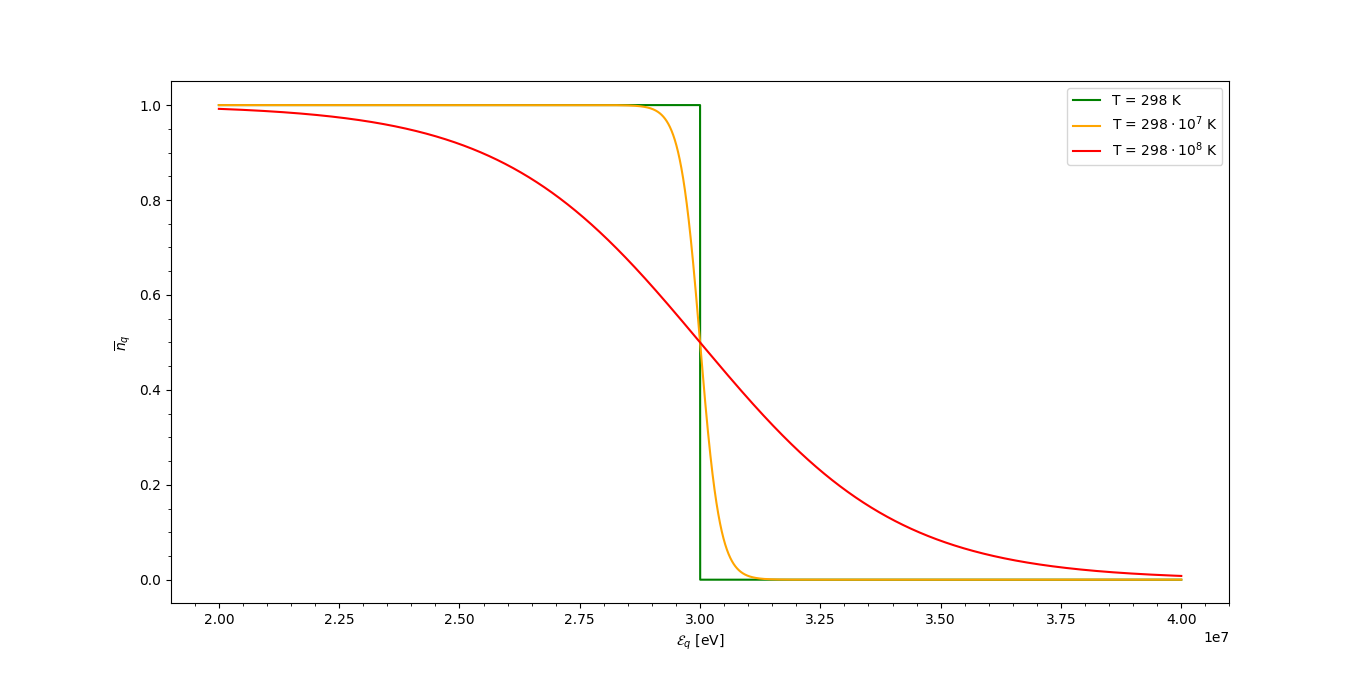
\includegraphics[width=0.9\textwidth]{figures/fermi_dirac.png}
	\caption{\scriptsize Distribuzione di fermi dirac realizzata in python per varie temperature e per $\mu = 30$ MeV, tipico dei gas di elettroni atomici.}
	\label{fig:figures-fermi_dirac-png}
\end{figure}
\noindent
Notiamo come a basse temperature ($kT \ll \mu$) la funzione sia praticamente un gradino che crolla sulla $\mu$, in questo caso lo smusso del gradino è proprio dell'ordine di $kT$.\\
Di fatto a $T\approx 0$ si ha che le particelle si dispongono in modo da minimizzare l'energia (andranno nei livelli energetici più bassi), quindi se voglio aggiungere una particella al sistema dovrò aggiungerla con una energia maggiore di quella delle particelle già presenti perchè tutti gli stati con energia inferiore sono occupati. Quindi per aggiungere questa particella dorvò dare una energia di almento $\mu$. L'energia $\mu = \mathcal{E}_{0}$ a temperatura nulla rappresenta di fatto la linea di demarcazione tra gli stati occupati e gli stati vuoti.\\
Questo ci da informazioni sul fatto che, se $T \to 0$, il potenziale chimico non potrà essere negativo perchè in tal caso il numero di particelle medio per ogni stato è nullo, quindi sparirebbero tutte le particelle dal sistema.\\
Ricordiamo che stiamo sempre considerando il sistema all'equilibrio con un bagno termico in cui abbiamo tenuto $\mu $ costante \footnote{Questo a livello fisico significa poter variare il numero di particelle al variare della temperatura, infatti il potenziale chimico è la variazione dell'energia del sistema rispetto al numero di particelle: per mantenerlo costante al variare dell'energia serve che cambi il numero di particelle.}, variare la temperatura significa variare la temperatura di questo "universo".\\
Spesso nei sistemi veri dobbiamo tener di conto che il numero di particelle del sistema in considerazione (bagno termico escluso) potrebbe essere fissato. In questo caso la legge resta valida però $\mu$ non è più fissato.\\
In questo caso possiamo aspettarci che esista una temperatura oltre il quale torniamo nella approssimazione classica di Boltzmann quindi il potenziale chimico dovrà tornare negativo e molto grande. \\
Possiamo dire anche qualcosa in più sul numero di particelle totali per questa distribuzione:
\[
	N = \sum_{q}^{} \overline{n}_{q} = \int_{0}^{\infty} \rho ( \mathcal{E} ) \cdot \frac{1}{\exp\left( \frac{\mathcal{E} -\mu }{kT} + 1 \right) } d\mathcal{E} 
.\] 
\paragraph{Distribuzione di Bose-Einstein e Bosoni}%
Nel caso in cui le particelle abbiano spin intero non abbiamo più nesuna condizione sulla occupazione degli stati, quindi non possiamo più tagliare al secondo termine nella sommatoria \ref{eq:Landau-Generic}, possiamo invece fare un cambio di variabile:
\begin{align}
	x = \exp\left( \frac{\mu -\mathcal{E} }{kT} \right) \implies
	\Omega _{q} = -kT \ln \left[ \sum_{n_{q}}^{} x^{n_{q}} \right] 
.\end{align}
Sappiamo che per non esplodere questa serie geometrica necessita che $x<1$, quindi che $\mu < \mathcal{E} _{q}$.
L'ultima disuguaglianza deve essere vera per tutti gli $\mathcal{E}_{q}$, quindi nel caso peggiore per lo stato con $\mathcal{E} = 0$, abbiamo allora una condizione sul potenziale chimico per la convergenza della serie:
\[
	\mu < 0
.\] 
Questo ci va bene perchè è conforme con quanto detto per il regime classico, dove anche in quel caso $\mu$ doveva essere negativo (in tal caso c'era una ulteriore condizione: doveva essere molto negativo).\\
Visto che la serie per $\Omega _{q}$ è geometrica si ha che la somma vale:
 \[
	 \Omega _{q} = kT \ln\left( 1-\exp\left( -\frac{\mathcal{E} _{q}-\mu }{kT} \right)  \right) 
.\] 
Quindi ci ricaviamo il numero medio di particelle: 
\[
	\overline{n}_{q} = - \frac{\partial \Omega _{q}}{\partial \mu } = \frac{1}{\exp\left( \frac{\mathcal{E} _{q}- \mu }{kT} \right)-1 }
.\] 
Abbiamo ottenuto una distribuzione simile alla Fermi-Dirac con un segno diverso, quel segno cambia pesantemente la forma della distribuzione che chiameremo:
\begin{defn}[Distribuzione di Bose-Einstein]{def:Distribuzione di Bose-Einstein}
	Il numero medio di particelle negli stati di singola particella $q$ per un gas di bosoni è dato da:
	\[
		\overline{n}_{q} = \frac{1}{\exp\left( \frac{\mathcal{E} _{q}-\mu}{kT} \right) - 1}
	.\]
\end{defn}
Graficamente la distribuzione con $\mu$ fissato è così fatta:
\begin{figure}[H]
	\centering
	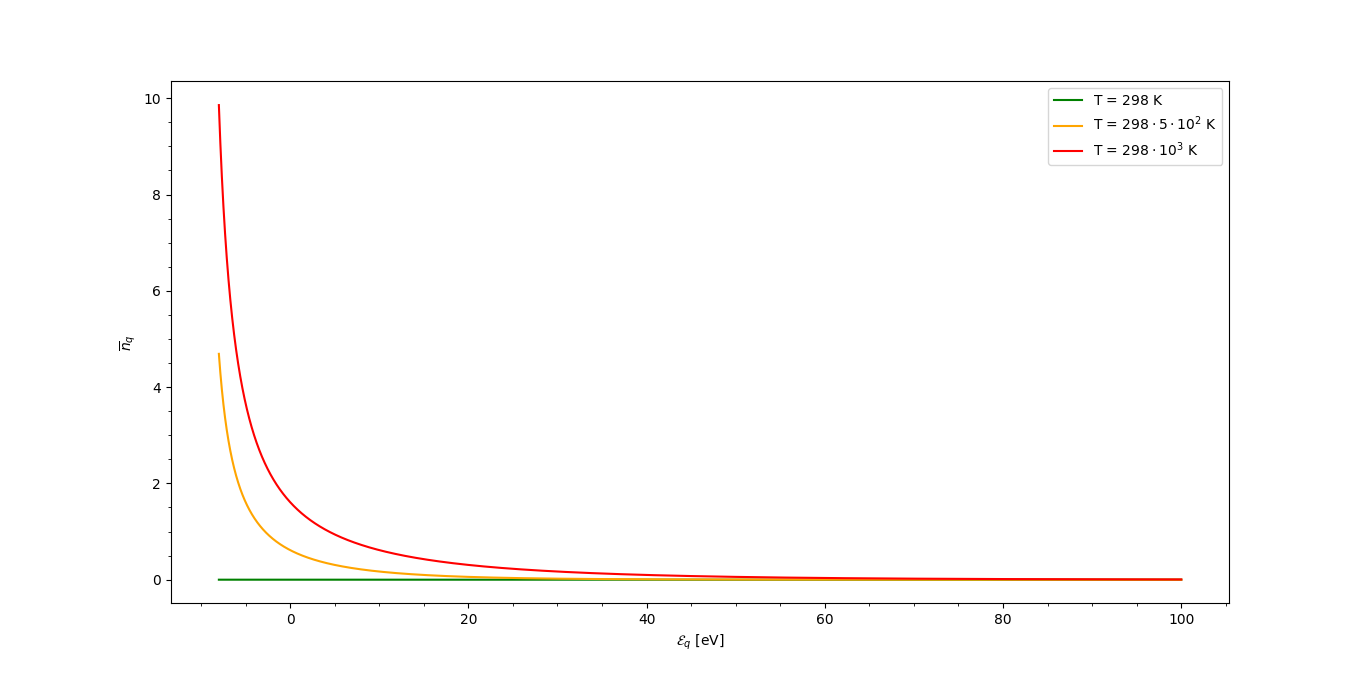
\includegraphics[width=0.95\textwidth]{figures/bose_einstein.png}
	\caption{\scriptsize Distribuzione di Bose-Einstein per $\mu = -10$ eV fissato.}
	\label{fig:figures-bose_einstein-png}
\end{figure}
\noindent
Questa è la Bose Einstein, e le particelle di spin intero sono perciò detti Bosone.\\
Tenere $\mu $ fissato anche in questo caso significa tenere libero il numero di particelle del sistema che quindi potrà essere scambiato con il bagno termico. La conseguenza che ne risulta dal grafico è che al diminuire della temperatura le particelle tenderanno a scappare dal sistema per spalmarsi in tutto l'universo (nei livelli di energia più bassa disponibili).\\
Nel limite classico entrambe le distribuzioni tornano al limite di Boltzmann classico.

\lez{8}{04-03-2020}{}
Abbiamo visto nella scorsa lezione che per un gas di Bosoni che può scambiare particelle con il bagno termico se la temperatura tende a zero allora numero di particelle medie per cella tende a zero: il sistema si svuota.\\
Noi considereremo più spesso casi in cui il numero di particelle è fissato, in tal caso il potenziale chimico diventa una funzione della temperatura.\\
Siccome il numero totale di particelle è dato da:
\[
	\int_{0}^{\mathcal{E} } \rho ( \mathcal{E} ) \overline{n}( \mathcal{E} ) d\mathcal{E} = N 
.\] 
È necessario che il potenziale chimico cresca e tenda quindi a zero cercando di mantenere costante l'integrale sotteso alla curva per energie positive.
\begin{figure}[H]
    %This is a custom LaTeX template!
    \centering
    \incfig{bose-einstein-con-t-tendente-a-zero-e-numero-di-particelle-fissato}
    \caption{\scriptsize Bose-Einstein con T tendente a zero e numero di particelle fissato.}
    \label{fig:bose-einstein-con-t-tendente-a-zero-e-numero-di-particelle-fissato.}
\end{figure}
\noindent
Quindi a $T=0$ abbiamo che l'unico stato occupato è lo stato fondamentale. Prossimamente discuteremo l'andamento di $\mu $ al variare di T, vedremo che $\mu $ diventa effettivamente zero per una temperatura di poco maggiore dello zero assoluto, raggiungendo uno stato della materia in cui il numero di particelle nello stato fondamentale è macroscopico \footnote{detto condensato di Bose-Einstein}.
\subsection{Fluttuazioni quantistiche vs fluttuazioni termodinamiche}%
Nella derivazione delle due distribuzioni abbiamo effettuato con leggerezza il passaggio al continuo, dovremmo almeno verificare che questo passaggio è lecito avendo abbandonato il regime di gas ideale.\\
Se chiamiamo $\delta \mathcal{E} $ la distanza media tra gli stati dobbiamo verificare che:
\[
	\delta \mathcal{E} \ll \sqrt{\overline{\left( \Delta \mathcal{E}  \right) ^2}} 
.\] 
In questo modo le fluttuazioni termodinamiche sono più importanti delle fluttuazioni quantistiche e ci è permesso fare un passaggio al continuo come già argomentato.\\
Le fluttuazioni termodinamiche dell'energia della singola particella sono dell'ordine di $kT$, mentre quelle quantistiche  $\frac{\hbar^2}{2m}\left( \frac{2\pi}{L} \right) ^2$ (nel caso di particelle confinate in una scatola di dimensioni caratteristiche linearri L).\\
Se prendiamo $L \approx 1cm$, $m \sim 10^{-24}g$ otteniamo che per avere $\overline{\left( \Delta \mathcal{E}  \right) ^2}\gg \delta \mathcal{E} $ serve $T> 10^{-10}K$. Per questo motivo in sistemi fisici reali non abbiamo problemi di fluttuazioni quantistiche.\\

\subsection{Spin nel calcolo della $\rho ( \mathcal{E} ) $}%
Quando a partire dagli impulsi siamo passati all'energia nella sezione \ref{subsec:dens-stati} ci siamo dimenticati dello spin che è un'altra variabile delle nostre particelle. Sappiamo che la degenerazione di spin è $2s+1$ \footnote{Dove $s$ è lo spin appunto}. Quindi se chiamiamo la densità di stati senza considerare lo spin $\rho '( \mathcal{E} ) $ si ha che la correzione dovuta allo spin su questa è: 
\[
	\rho ( \mathcal{E} ) = \rho'( \mathcal{E} ) \cdot  \left( 2s + 1 \right)   = g \rho '( \mathcal{E} ) 
.\] 
Visto che noi parliamo di fermioni e bosoni le nostre correzioni sono relativamente 2 e 1, fatta eccezione per i fotoni ed i fononi \footnote{Questi ultimi si occupano delle vibrazioni dei cristalli, sono quanti o quasi-particelle.}.
Infatti nel caso dei fononi abbiamo tre degenerazioni dovute ai gradi di liberta vibrazionali, mentre per i fotoni sappiamo invece che abbiamo due degenerazioni dovute alle possibili polarizzazioni.\\
La densità di stati che continueremo ad usare per qualche lezione è quella ricavata nella sezione citata sopra:
\[
	\rho ( \mathcal{E} ) d\mathcal{E} = \frac{4\pi\sqrt{2} V m_{3 /2}}{\left( 2\pi \hbar \right)^3 } \mathcal{E} ^{1 /2} g d\mathcal{E} 
.\] 
Relativa ad un sistema tridimensionale di particelle con energia $p^2/2m$.

\subsection{Correzione al secondo ordine per l'equazione di stato dei gas ideali}%
Cerchiamo di capire cosa succede quando siamo in condizioni tali da non poter usare l'approssimazione di gas ideali "per poco" quindi quando la disuguaglianza \ref{eq:ideal_gas_approx} non è forte, ma è soltanto una disuguaglianza.\\ 
Per farlo andiamo all'ordine successivo nelle approssimazioni fatte con quella disuguaglianza, che ricordiamo essere:
\[
	\exp\left( \frac{\mu }{kT} \right) \ll 1
.\] 
Quindi vediamo come si modifica l'equazione di stato dei gas ideali quando iniziamo a tener di conto degli effetti quantistici.\\
Il potenziale di Landau nei due casi studiati sopra è:
\[
	\Omega^{\text{FD}}_{\text{BE}} = \mp kT \sum_{q}^{} \ln\left[ 1 \pm \exp\left( - \frac{\mathcal{E} _{q}-\mu }{kT} \right)  \right] 
.\] 
Dove il segno superiore è per la Fermi-Dirac, il segno inferiore è per la Bose-Einstein.\\
Per arrivare alla approssimazione classica nella abbiamo tenuto soltanto i termini al primo ordine in $x$, adesso usando l'espressione di $\Omega$ per bosoni e fermioni possiamo anche andare al secondo ordine $x^2$:
\[
	\Omega = -kT \sum_{q}^{} \exp\left( - \frac{\mathcal{E} _{q}-\mu }{kT} \right) \pm \frac{kT}{2}\sum_{q}^{} \exp\left[ - \frac{2 \left( \mathcal{E} _{q}-\mu  \right) }{kT} \right] 
.\]
Mentre la prima parte è il potenziale di Landau già trovato in ambito classico il secondo pezzo inizia a differenziarsi nel caso si tratti di fermioni o bosoni:
\[
	\Omega = \Omega _{\text{class}} \pm \frac{kT}{2}\sum_{q}^{} \exp\left[ - \frac{2 \left( \mathcal{E} _{q}-\mu  \right) }{kT} \right] 
.\]
Possiamo fare il conto della correzione passando al continuo visto la valutazione sulle fluttuazioni fatta due sezioni sopra:
\[
	\sum_{q}^{} \exp\left( -\frac{2\mathcal{E} _{q}}{kT} \right) = \int_{0}^{\infty}  \rho ( \mathcal{E} ) \exp\left( - \frac{2\mathcal{E} }{kT} \right) d\mathcal{E} =
	\left( \frac{1}{2} \right) ^{3 /2}\int_{0}^{\infty} \rho ( \overline{\epsilon }) \exp\left( - \frac{\overline{\epsilon }}{kT} \right) d \overline{\epsilon } 
.\] 
Dove abbiamo fatto il cambio di variabile $\overline{\epsilon }= 2\mathcal{E} $, abbiamo inoltre considerato il fatto che in $\rho ( \mathcal{E} ) \propto \mathcal{E} ^{1 /2}$ quindi esce quel fattore alla $3 /2$ dall'integrale.
Quindi la correzione alla $\Omega _{\text{class}}$ è la seguente:
\[
	\pm kT \left( \frac{1}{2} \right) ^{5 /2} \exp\left( \frac{\mu }{kT} \right) \int_{0}^{\infty} \rho ( \overline{\epsilon }) \exp\left( - \frac{\overline{\epsilon }}{kT} \right) d \overline{\epsilon } 
.\] 
Notiamo adesso che la maggior parte della correzione che abbiamo ottenuto non è altro che $\Omega _{\text{class}}$ stessa, possiamo allora compattare l'espressione raggruppando questa quantità (ponendo attenzione ai segni):
\[
	\Omega = \Omega _{\text{class}} \left[ 1 \mp \frac{\exp\left( \frac{\mu }{kT} \right) }{2^{5 /2}} \right] 
.\] 
Siamo pronti a ricavare l'equazione del gas perfetto con effetti quantistici:
\[
	\Omega  = - PV
.\]  
\[
	\Omega _{\text{class}} = -NkT
.\]
allora avviamo la correzione
\[
	PV = NkT\left[ 1 \mp \frac{\exp\left( \frac{\mu }{kT} \right) }{2^{5 /2}} \right] \label{eq:eq-id-corretta_1}
.\] 
Possiamo chiederci se questa correzione ha senso, alla luce del fatto che la correzione per i fermioni è negativa e che per questi non possiamo avere più di una particella per stato. Una forma equivalente è la seguente:
\[
	P = \frac{N}{V} kT \left[ 1 -+ \frac{\exp\left( \frac{\mu }{kT} \right) }{2^{ 5 /2}} \right] 
.\] 
Quindi per un gas di fermioni alla temperatura T con densità $N /V$ la pressione è inferiore a quella di un gas classico, mentre per un gas di bosoni la pressione la pressione è inferiore. \\
Questo è assolutamente contro intuitivo: i fermioni (che hanno al massimo una particella per stato) ci aspettiamo abbiano una "repulsione intrinseca" maggiore dei bosoni che non hanno problemi ad ammassarsi negli stati a bassa energia. Di conseguenza ci si aspetta anche che per i fermioni la pressione sia maggiore che per i gas ideali e viceversa per i bosoni. \\
Il segno del secondo termine nella \ref{eq:eq-id-corretta_1} dovrebbe essere allora invertito per soddisfare il nostro intuito. Tuttavia la derivazione che abbiamo seguito sembra corretta, non ci sono evidenze di errori algebrici. Deve esserci qualcosa di concettualmente sbagliato quindi.\\
Possiamo provare con un'altra derivazione passando questa volta dalla energia libera F, ricordiamo la proprietà che lega le variazioni dei potenziali termodinamici durante una trasformazione sul sistema:
\[
	\left.\delta F\right|_{T,V,N} = \left.\delta \Omega \right|_{T,V,\mu }
.\]
La variazione che consideriamo è la correzione da sistema classico a sistema "leggermente quantistico" come spiegato all'inizio.
Possiamo scrivere che:
\[
	\Omega ( T,V,\mu )  = \Omega _{\text{class}} + \delta \left.\Omega \right|_{T,V,\mu }
.\] 
Con $\left.\delta \Omega \right|_{T,V, \mu}$ che è quella calcolata prima. Avremo di conseguenza per la F:
\[
	F( T,V,N) = F_{\text{class}} + \left.\delta F\right|_{T,V,N}
.\] 
Quindi la correzione trovata per il potenziale di Landau sarà la stessa di quella per l'energia libera, l'unica accortezza da tenere è che nel primo caso era fissato il potenziale chimco, nel secondo il numero di particelle. Vedremo che la chiave del "mistero" sopra sarà esattamente questa.\\
Abbiamo trovato che:
\[
	\delta \Omega = \mp \Omega _{\text{class}}\frac{\exp\left( \mu  \right)kT }{2^{5 / 2}} = \pm NkT \frac{\exp\left( \frac{\mu }{kT} \right) }{2 ^{5 /2}}
.\] 
Quello che vorremmo fare adesso è eliminare la dipendenza esplicita da $\mu $ di questa correzione per poterla sostituire in F in funzione delle sue variabili predilette, per farlo ricordiamo l'equazione \ref{eq:mu_classico} del caso classico:
\[
	\mu _{\text{class}} = -kT \ln\left( \frac{V}{N\Lambda ^3} \right) 
.\] 
Per toglierci di mezzzo $\mu $ basterà sostituirlo in $\delta \Omega $, infatti la correzione su $\mu _{\text{class}}$ inserita all'interno della variazione sul potenziale di Landau genera una correzione all'ordine successivo che possiamo trascurare. Dalla sostituzione si ricava che:
\[
	F = F_{\text{class}} \pm \frac{N^2kT\Lambda ^3}{2^{5 /2}V}
.\] 
Quindi ricaviamo la legge di stato:
\[
	P = - \frac{\partial F}{\partial V} = P_{\text{class}} \pm \frac{N^2kT\Lambda ^3}{2^{5 /2}V^2} = \frac{NkT}{V}\left( 1 \pm \frac{N\Lambda ^3}{2^{5 /2}V} \right) 
.\] 
Abbiamo ottenuto i segni che intuitivamente ci si aspetterebbe, resta tuttavia il problema che i due metodi hanno prodotto risultati all'apparenza contrastanti.\\
Nel primo caso abbiamo trovato la pressione da $\Omega $, nel secondo partendo da $F$. Ragionando con la $\Omega $ il numero di particelle non è costante durante una compressione. Questo ci porta in errore quando facciamo ragionamenti di intuito come abbiamo fatto sopra. Il modo giusto (nel quale ha senso applicare il nostro ragionamento) è quello di partire dalla $F$. Infatti quello che ci aspettiamo fisicamente è che, durante una compressione, il numero di particelle resti invariato.\\
Resta il fatto che non abbiamo trovato l'inghippo matematico alla base del problema, infatti quello che abbiamo fatto nel secondo caso è prendere la correzione calcolata con $\Omega $ ed inserirla nell'espressione per $F$, quindi l'errore avrebbe dovuto comparire anche alla fine del secondo ragionamento.\\ 
Dobbiamo stare attenti al fatto che nel primo caso $N = N ( \mu ) $ ed in particolare si ha che, fissato un $\mu $:
\[
N = N_{\text{class}}( \mu ) \neq N_{2^o\text{ordine}}( \mu ) 
\]
Abbiamo quindi un abuso di notazione, il numero di particelle $N$ che consideriamo per il nostro sistema non è più quello classico ma è anch'esso corretto al secondo ordine.\\
Quindi quando facciamo la differenza rispetto alla funzione classica e cerchiamo di capire se ci tornano le considerazioni su fermioni e bosoni sbagliamo nel fatto il numero di particelle non è lo stesso rispetto al caso classico.\\
Non possiamo dire lo stesso del secondo caso, infatti il numero di particelle in  $F$ è fissato, il chè non ci porta in errore quando sostituiamo l'equazione dei gas perfetti per eliminare $P_{\text{class}}$.

\subsection{Gas di Fermioni: elettroni di conduzione in un metallo}%
Riprendiamo la distribuzione di Fermi-Dirac per trattare un gas di elettroni in un metallo.\\
La prima cosa da fare è calcolare il numero di particelle $N$ :
\[
	N = \int_{0}^{\infty} \frac{\rho ( \mathcal{E} ) d\mathcal{E} }{\exp\left( \frac{\mathcal{E} -\mu }{kT}+1 \right) }
.\] 
Normalmente questo sarebbe integrato da $0$ ad $\infty$, nel limite di $T \to 0$ si può approssimare la distribuzione da un gradino unitario, quindi:
\[
	N \to \int_{0}^{\mathcal{E} _{F}}  \rho ( \mathcal{E} ) d\mathcal{E}  
.\] 
Quindi possiamo, anzichè integrare la $\rho ( \mathcal{E} ) $ brutta, possiamo prendere il volume della sfera nello spazio delle fasi di raggio $p _{F}$ tale che $\mathcal{E} _{F} = p_{F}^2 /2m$, moltiplicarlo per il volume in questione $V$, dividere per il volume della cella unitaria (senza scordarsi dello spin).
\[
	N = \frac{g V \left( \frac{4}{3} \pi p_{F}^3 \right) }{\left( 2\hbar \pi \right) ^3} 
.\] 
Possiamo ricavare $p_{F}$ da quest'ultima oppure direttamente $\mathcal{E} _{F}$ dall'integrale, quello che si ottiene è sempre:
\[
	\mu _{0} = \mu ( 0) = \mathcal{E} _{F} = \frac{\left( 2\pi \hbar  \right) ^2}{2m} \left( \frac{N}{V} \right) ^{2 /3} \left( \frac{3}{4\pi q} \right) ^{2 /3}
.\]
Possiamo trovare l'energia media a $T\to 0$:
\[
	\overline{\mathcal{E} } = \frac{\int_{0}^{\mathcal{E} _{F}} \mathcal{E} \rho ( \mathcal{E} ) d\mathcal{E} }{\int_{0}^{\mathcal{E} _{F}} \rho ( \mathcal{E} ) d\mathcal{E}  }=
	\frac{\int_{0}^{\mathcal{E} _{F}} \mathcal{E} ^{3 /2}d\mathcal{E}  }{\int_{0}^{\mathcal{E} _{F}} \mathcal{E} ^{ 1/ 2}d \mathcal{E}  } = 
	\frac{3}{5} \mathcal{E} _{F}	
.\] 
Di conseguenza l'energia totale sarà:
\[
	E( T=0)  = N \overline{\mathcal{E} } = \frac{3}{5} \mathcal{E}_{F} N
.\] 
Mentre la pressione è data da:
\[
	P = - \left.\frac{\partial E}{\partial V} \right|_{N} = \frac{2}{3}\frac{E}{V}
.\] 
Quest'ultima l'avevamo già ricavata a partire dal fatto che la legge di dispersione dell'energia è $p^2/2m$, senza nessuna assunzione. Notiamo che la pressione a $T = 0$ non va a zero. Questo non succede per il gas classico.\\
Vediamo invece come cambiano le cose se la temperatura non è nulla ma vale 
\[
T \ll T_{F} 
\]
Dove $T_{F}$ è la temperatura definita a partire da $kT_{F} = \mathcal{E} _{F}$, ed è detta temperatura di Fermi. Visto che abbiamo espresso $\mathcal{E} _{F}$ possiamo esprimere anche $T_{F}$
\[
	T_{F} = \frac{\left( 2\pi \hbar  \right)^2}{2m k} \left( \frac{3}{4\pi q} \right)^{2 /3} \left( \frac{N}{V} \right) ^{2 /3}
.\] 
Per $T\ll T_{F}$ si ha che la distribuzione di Fermi è molto simile al gradino, questo ci permetterà di fare delle approssimazioni. Vediamo adesso con un esempio pratico se in condizioni normali tale disuguaglianza è rispettata.\\
Visto che conosciamo la densità di elettroni liberi in un metallo possiamo calcolare la $T_{F}$ di quest'ultimo. Nel rame abbiamo ad esempio $\rho _{e}= 8.5 \cdot 10^{22}$ e/cm$^3$, messa nella formula per la temperatura di Fermi ci restituisce:
\[
	T_{F, \text{rame}} = 8.5 \cdot 10^{4} K
.\] 
Se ne conclude che a temperatura ambiente siamo sempre nel regime $T \ll T_{F}$.\\
Tipicamente la $T_{F}$ è maggiore della temperatura di fusione dei metalli. Questo ci dice che gli elettroni nei metalli sono essenzialmete quantistici, abbiamo una distribuzione di questi nei livelli completamente diversa da quella prevista da Boltzmann.
\begin{defn}[Gas Degenere]{def:Gas Degenere}
	Un gas si dice degenere quando si trova in un regime in cui non vale più l'approssimazione di gas ideale, tale gas sarà quindi descritto da una distribuzione non classica come la Fermi-Dirac oppure la Bose-Einstein.\\
	Sono ad esempio degeneri gli elettroni di un metallo.
\end{defn}
Abbiamo tuttavia delle precisazioni da fare, poichè gli elettroni in un metallo non solo fanno cadere l'approssimazione di gas ideale ma potrebbero uscire anche dalla approssimazione di gas perfetto!\\
Infatti stiamo operando in situazioni in cui questi sono degeneri (quindi il più compatti possibile nei limiti imposti dalla Fermi-Dirac), la loro vicinanza ci induce a pensare che non si possa più trascurare l'interazione coluombiana. Inoltre sono all'interno di un metallo che idealmente sta perdendo elettroni in continuazione, quindi saranno immersi in una miriade di ioni che sono un'altra possibile fonte di interazione.\\
Fortunatamente la situazione si risolve assumendo che gli elettroni abbiano lunghezze d'onda grandi rispetto alla distanza tra gli atomi del solido.\\
In questo modo gli elettroni è come se vedessero un background di carica uniforme proveniente da tutti gli ioni, questo può essere il fondo della buca di potenziale dato dalla scatola \footnote{In questo ragionamento il "confinamento" dovuto alle pareti della scatola ed il background di ioni sono la stessa cosa!}. Inoltre il fondo positivo scherma l'interazione culoumbiana tra gli elettroni, quindi in questa ottica possiamo tenerci gli elettroni come gas perfetto.\\
Ci aspettiamo inoltre che gli elettroni possano comunque scatterare o interagire per collisioni, tuttavia se $T \ll T_{F}$ questi fermioni non avranno comunque livelli liberi per cambiare la loro energia qualunque tipo di interazione facciano. \\
Possiamo anticipare che i fenomeni di scattering coincolgeranno solo gli elettroni aventi energie prossime all'energia di fermi perchè sono gli unici ad avere un pò di stati vuoti nelle vicinanze per potersi spostare.\\
Essenzialmente, quando faremo il modello di gas di elettroni nei solidi, potremo trattare tutto come un gas perfetto, l'unica cosa che cambia è che la massa nella relazione:
\[
	\mathcal{E} = \sum_{}^{} \frac{P^2}{2m}
.\] 
Non sarà la massa dell'elettrone libero, sarà una massa efficace che tiene conto del fatto che gli elettroni non si muovono in uno spazio vuoto ma sono "vincolati" in uno spazio occupato da altri elettroni e nuclei.\\
Storicamente il fatto che all'interno dei metalli vi fossero elettroni liberi fu accolto in modo positivo dalla comunità scentifica che iniziò subito ad attrezzarsi per misurare e verificare questo fatto.\\ 
I fisici tirarono fuori una densità media di elettroni all'interno del metallo facendo delle misure, furono quindi in grado di tirare fuori un calore specifico sperimentale. Essi si aspettavano che il calore specifico per questo gas di particelle libere nel metallo fosse quello classico: 
\[
	C_{V}= \frac{3}{2}Nk
.\] 
Quest'ultima risultò incompatubile con le misure. Il calore specifico ottenuto era molto inferiore di quello atteso. Noi sappiamo che il motivo proviene dal fatto che la statistica non è più quella di Boltzmann. \\
Se ad esempio consideriamo la statistica di Fermi-Dirac per $T \approx 0$ ed aumentiamo di poco la temperatura si ha che gli unici elettroni che cambiano energia sono quelli che stanno in un intorno largo $kT$ dell'energia di fermi, per tutti gli altri non cambia assolutamente nulla.\\ 
Ci aspettiamoche il numero totale di elettroni che contribuiscono al calore specifico non sia $N$ ma sia solo una frazione:
\[
	N_{C_{V}} \sim N\cdot \frac{T}{T_{F}}
.\] 
Il guadagno di energia di questi elettroni per fare un salto di energia sarà:
\[
	\Delta E = \frac{N kT^2}{T_{F}}
.\] 
Quindi per definizione di calore specifico si ha che:
\[
	C_{V} \approx \frac{\Delta E}{\Delta  T} = \alpha \frac{T}{T_{F}} 
.\] 
In effetti si riscontra che il calore specifico nei metalli ha proprio questo andamento lineare nella temperatura.\\
Cerchiamo di sviluppare le proprietà termiche del gas di elettroni, le useremo per esempio per descrivere il calore specifico. Non faremo più gli integrali in modo da approssimare la Fermi-Dirac come funzione a gradino ma ci teniamo l'espressione con la dipendenza dalla temperatura.
\[
	\Omega = -\frac{2}{3} \frac{4\pi V g \sqrt{2}  m ^{3 /2}  }{\left( 2\pi\hbar  \right) ^3} \int_{0}^{\infty} \frac{\mathcal{E} ^{3 /2}d\mathcal{E} }{\exp\left( \frac{\mathcal{E} -\mu }{kT} \right) +1 } 
.\] 
Siamo comunque nelle ipotesi in cui $T\ll T_{F}$, quindi cercheremo di riscrivere l'integrale di sopra con una correzione all'ordine opportuno in questo modo:
\[
	I = \int_{0}^{\infty} \frac{f( \mathcal{E} ) }{\exp\left( \frac{\mathcal{E} -\mu }{kT} \right) +1 }d\mathcal{E}  = I_0 + \delta  I 
.\] 
Dove il termine $I_0$ introdotto è:
\[
	I_0 = \int_{0}^{\mathcal{E} _{F}} f( \mathcal{E} ) d\mathcal{E} 
.\] 
Cercheremo di fare una espansione di $I$ in funzione della temperatura:
\[
	I = I_0 + \left.\frac{\partial I}{\partial T} \right|_{T =0} + \frac{1}{2}\left.\frac{\partial ^2I}{\partial T^2} \right|_{T = 0} T^2 + \ldots
.\] 
Prima di procedere dobbiamo chiederci se ci basta una correzione al primo ordine o se dobbiamo correggere con ordini successivi. Questo possiamo capirlo dalla forma della distribuzione nell'intorno della energia di fermi:
\begin{figure}[H]
    %This is a custom LaTeX template!
    \centering
    \incfig{correzione-per-il-potenziale-di-landau-nella-statistica-di-fermi-dirac}
    \caption{\scriptsize Correzione per il potenziale di Landau nella statistica di Fermi-Dirac, in tratteggiato la curva con $T=0$, in continuo la linea con $T\ll T_{F}$}
    \label{fig:correzione-per-il-potenziale-di-landau-nella-statistica-di-fermi-dirac}
\end{figure}
\noindent
La variazione sull'area $I$ cercata sarà la differenza tra la curva tratteggata e la curva continua, possiamo vedere intuitivamente come al primo ordine questa differenza debba annullarsi per simmetria. Per questo la correzione al primo ordine si annulla, quindi al primo ordine $N$ resta costante.\\ 
Per calcolare le correzioni al secondo ordine facciamo un cambio di variabile: passiamo da $\mathcal{E} $ a $z = \exp\left( \frac{\mathcal{E} -\mu }{kT} \right) $ ed introduciamo due funzioni: 
 \begin{align*}
	&g_1( z)  = \begin{cases}
		0 \quad z <0\\
		\frac{1}{e^{z}+1} \quad z > 0
	\end{cases}\\
	&g_0( z) =
 \begin{cases}
		\frac{1}{e^{-z}+1} \quad z < 0 \\
		0 \quad z >0
	\end{cases}
.\end{align*}
Vediamo che queste non sono altro che le due "fette" che differiscono tra la distribuzione a temperatura nulla e quella a temperatura molto bassa, soltanto che la $g_0$ è la parte in alto ribaltata:
\begin{figure}[H]
    %This is a custom LaTeX template!
    \centering
    \incfig{g1-e-g0}
    \caption{\scriptsize Plot delle due funzioni scritte sopra.}
    \label{fig:g1-e-g0}
\end{figure}
La differenza dell'integrale della fermi dirac tra $T=0$ e  $T\ll T_{F}$ sarà dato da:
\[
	\delta I = \int_{-\infty}^{\infty} f( \mathcal{E} ) \left[ g_1( z) - g_0( z)  \right] d\mathcal{E}   = \int_{-\infty}^{\infty}  f ( \mu + kTz) 
	\left[ g_1( z) - g_0( 0)  \right] kT dz
.\] 
L'estremo inferiore di integrazione sarebbe dato dal fatto che $\mathcal{E} _{\text{min}}=0 \implies z_{\text{min}}= - \mu /kT$, tuttavia possiamo anche mandarlo a $-\infty$ poichè per il valore di $z_{\text{min}}$ la differenza tra le $g_{i}$ è praticamente ormai nulla, quindi andare a $-\infty$ non compromette il risultato della somma.\\
Procediamo al calcolo dell'ultimo integrale, dal momento che l'integrale è pesato solo attorno al potenziale chimico possiamo sviluppare $f( \mu + kTz) $ attorno a $0$:
\[
	f( \mu + kTz) = f( \mu )  + kTz \left.\frac{\partial f}{\partial \mathcal{E}  } \right|_{\mathcal{E} =\mu } + \ldots= f( \mu )+ kTzf'( z)  
.\] 
Sostituendo troviamo:
\[
	\delta I = kTf( \mu )  \int_{-\infty}^{\infty} \left[ g_1( z)- g_0( z)   \right] dz + ( kT) ^2f'( z) \int_{-\infty}^{\infty} z \left[ g_1( z) -g_0( z)  \right] dz  
.\] 
Quindi aver fatto lo sviluppo attorno al potenziale chimico della $f$ è stato equivalente a fare lo sviluppo agli ordini successivi della temperatura di $\delta I$.\\
Il primo pezzo (che è il primo ordine) è esattamente zero perchè le due aree delle $g_{i}$ si elidono in questi estremi di integrazione per simmetria. Il secondo pezzo avendo z nell'integrale "rompe la simmetria" delle $g$ permettendo così che si sommino i contributi di queste due.

\end{document}
